\documentclass{report}
\usepackage{algorithm}
\usepackage{titlesec}
\usepackage[T1]{fontenc} % Use 8-bit encoding that has 256 glyphs
\usepackage[english]{babel} % English language/hyphenation
\usepackage{amsmath,amsfonts,amsthm} % Math packages
\usepackage{lipsum}
\usepackage{caption}
\usepackage{subcaption}
\usepackage{graphicx}
\usepackage{tocloft}
\usepackage{float}
\usepackage{blindtext} %for enumarations
\usepackage[hidelinks]{hyperref}
\usepackage{graphicx}  % For including images
\usepackage{color}    
\usepackage{xcolor}    
\usepackage{fancyhdr}
\usepackage{acronym}
\usepackage[a4paper, margin=1.1in]{geometry}
%\usepackage{sectsty} 
\usepackage{titlesec}
\usepackage{setspace}
\usepackage{booktabs}
\usepackage{nomencl}
\usepackage{glossaries}
\pagestyle{fancyplain} 
\usepackage{comment}
\usepackage{algpseudocode}
\usepackage{svg}
\usepackage{verbatim}
\usepackage{parskip}
\usepackage{url}
\usepackage{cite}
\usepackage[bottom]{footmisc}

\usepackage[table]{xcolor}
\definecolor{bestcell}{HTML}{C6EFCE}  
\definecolor{worstcell}{HTML}{FFC7CE}
% \definecolor{bestcell}{HTML}{6ABF8E}   % soft sage green
% \definecolor{worstcell}{HTML}{FFC7CE}  % light red (unchanged)
\fancyhf{}
\fancyfoot[C]{
    \vspace{1em}
    \hrule width \textwidth height 0.4pt
    \vspace{0.5em}
    \thepage
}
\setlength{\headheight}{13.6pt} 


\titleformat{\subsubsection}[block]
  {\normalfont\bfseries}
  {\thesubsubsection}
  {1em}
  {}
  
\numberwithin{equation}{chapter} 
\numberwithin{figure}{chapter} 
\numberwithin{table}{chapter}

\setlength\parskip{12pt}

%----------------------------------------------------------------------------------------
%	TITLE SECTION
%----------------------------------------------------------------------------------------
% Custom title page setup
\makeatletter
  \def\@title{\textcolor{red}{Title}}

  \def\@subtitle{\textcolor{red}{Subtitle}}
  \newcommand\subtitle[1]{\def\@subtitle{#1}}

  \def\@author{\textcolor{red}{Author}}

  \def\@studentnumber{\textcolor{red}{Student Number}}
  \newcommand\studentnumber[1]{\def\@studentnumber{#1}}

  \def\@supervisor{\textcolor{red}{Supervisor(s)}}
  \newcommand\supervisor[1]{\def\@supervisor{#1}}

  \def\@department{\textcolor{red}{Department}}
  \newcommand\department[1]{\def\@department{#1}}

  \def\@subjectcode{\textcolor{red}{SUBJECT CODE}}
  \newcommand\subjectcode[1]{\def\@subjectcode{\MakeUppercase{#1}}}

  \def\@subjectname{\textcolor{red}{Subject Name}}
  \newcommand\subjectname[1]{\def\@subjectname{#1}}

  \def\@degreename{\textcolor{red}{Degree}}
  \newcommand\degreename[1]{\def\@degreename{#1}}

  \def\@field{\textcolor{red}{Field}}
  \newcommand\field[1]{\def\@field{#1}}

  \def\@keywords{\textcolor{red}{Keywords}}
  \newcommand\keywords[1]{\def\@keywords{#1}}

  \def\@date{\today}

  \renewcommand{\maketitle}{
    \thispagestyle{empty}
    \begin{center}
      {\Huge \@title}
      \vskip 3mm
      \hrule
      {\Large }
      \vfill
      
      
\includegraphics[scale= 0.9]{Figure/UCT.jpg}
      \vfill

      Prepared by:
       \\[0.5cm]
       {\LARGE \@author}
        \\[0.2cm]
      \@studentnumber
      \vfill

      Supervised by:
      \\[0.5cm]
       {\LARGE \@supervisor}\\  
       Department of Electrical Engineering
      \vfill

      \textbf{\@date}
      \vfill
      
      A dissertation submitted to the Department of \@department \\
         \textbf{University of Cape Town},\\ 
         in partial fulfilment of the academic requirements \\
         for the degree of
         \vfill
         \textbf{\@degreename\ }
        
    \end{center}
    \clearpage
  }
\makeatother
\renewcommand{\footnoterule}{
    \vspace{1em} % Space above the line
    \hrule width \textwidth height 0.4pt
    \vspace{0.6em} % Space below the line
}

%\makeglossaries

\begin{document}
\date{March 18, 2026}                                                                                                     

% Set title, author, and other details
\title{Design and Implementation of Tracking Filters for a  Passive Radar System}
\author{I.J. Malemela}
\studentnumber{MLMITU002}
\supervisor{W.P.F. Schonken and S.T Paine}
\department{Electrical Engineering}
\degreename{MScEng Electrical Engineering Specializing in Radar }
\field{Engineering}
\keywords{Passive Radar, Tracking Filters}
\maketitle 
\pagenumbering{roman}

\newpage
\thispagestyle{empty}
\null
\setstretch{1.5}
\newpage
\addcontentsline{toc}{section}{Declaration}
{
  \makeatletter
    \thispagestyle{empty}
    \renewcommand{\thefootnote}{}
    \vspace*{3cm}
    \noindent \large \textbf{\Huge Declaration}
    \\[2cm]
    \noindent I know the meaning of plagiarism and declare that all the work in the document, save for that which is properly acknowledged, is my own. This thesis/dissertation has been submitted to the Turnitin module (or  equivalent similarity and originality checking software) and I confirm that my supervisor has seen my report and any concerns revealed by such have been resolved with my supervisor.
    \vspace{15mm}
    \vspace{15mm}\\
    \noindent Signature of Author \dotfill \\
    \noindent Cape Town \\
    \noindent \@date
    
  \makeatother
  \clearpage
}


\newpage
\addcontentsline{toc}{section}{Abstract}
\vspace*{3cm}
\noindent \large \textbf{\Huge Abstract}
\\[1.5cm]
Passive Radar, also referred to as Bistatic Radar, Passive Coherent Location, or Non-Cooperative Radar, utilizes existing transmitter infrastructure to detect targets based on their skin returns. The transmitters, also known as illuminators of opportunity, are uncooperative transmitters that are not explicitly dedicated for Passive Radar. Examples of such transmitters include Digital Audio Broadcasting, Frequency Modulated radio, Digital Video Broadcasting Terrestrial/Second Generation, Digital Video Broadcasting Satellite/Second Generation and cellular base transmitters.
\newline
\newline
Using FM Passive Radar to detect and visually follow the trajectories of targets presents several challenges, such as clutter, direct and multi-path interference, and poor range resolution. However, it also offers advantages, such as long integration times that allow for high Doppler resolution. Although extensive research has been conducted on tracking filters and their applications across multiple domains, there has been limited exploration on the application of various tracking filters to track commercial aircraft using FM radio signals.
\newline
\newline
 This research aims to explore, develop and implement various tracking filters that can track commercial aircraft using  Passive Radar data. The tracking filters' performance will be evaluated based on several parameters, including computational load, data association and the log-likelihood as a statistical benchmark. By investigating and implementing multiple tracking filters for Passive Radar, this project will contribute towards the advancement of Passive Radar tracking systems.

\newpage
\newpage
\addcontentsline{toc}{section}{Acknowledgements}
\vspace*{3cm}
\noindent \large \textbf{\Huge Acknowledgements}
\\[1.5cm]
I wish to extend my profound gratitude to my supervisors, Dr. Willem Schonken and Dr. Stephen Paine, for their invaluable guidance and unwavering support throughout the course of the Masters project. Their expertise and encouragement were instrumental in overcoming challenges and staying motivated.

To my partner, Mabatho Hashatsi, your constant support, patience, and faith in me have been my greatest source of strength. I am deeply grateful for your unwavering presence by my side every step of the way.

I extend my heartfelt appreciation to my former Radar Masters classmates and colleagues for their invaluable assistance in reviewing my work and providing constructive feedback, which greatly contributed to the refinement of this dissertation.

To my parents, I am grateful for your unwavering love and support, which have been the foundation of my strength throughout this journey. Above all, I extend my deepest gratitude to the Almighty Lord, whose grace and guidance have made this accomplishment possible.

\newpage
\renewcommand{\cfttoctitlefont}{\Huge \bf}
\addcontentsline{toc}{section}{Table of Contents}
\tableofcontents

\clearpage

\newpage
\setlength{\cftfignumwidth}{3em}
\newpage
\vspace*{2cm}
\addcontentsline{toc}{section}{List of Figures}
\listoffigures


\newpage
\setlength{\cfttabnumwidth}{3em} 
\newpage
\vspace*{2cm}
\addcontentsline{toc}{section}{List of Tables}
\listoftables


\vspace*{2cm}
\addcontentsline{toc}{section}{List of Algorithms}
\listofalgorithms




\newpage
\newpage
\vspace*{2cm}
\addcontentsline{toc}{section}{List of Abbreviations}
\noindent \large \textbf{\Huge List of Abbreviations}
\vspace*{1cm}

\newacronym{2D}{2D}{2-Dimensional}

\begin{acronym}[OSGO-CFAR] 
    \acro{2D}{2-Dimensional}
    \acro{3D}{3-Dimensional}

    \acro{ADC}{Analogue Digital Converter}
    \acro{ADS-B}{Automatic Dependant Surveillance-Broadcast}
    \acro{AIS}{Automatic Identification System}
    \acro{ARC}{Ames Research Center}
    \acro{ARD}{Amplitude/Range/Doppler}
    \acro{ATC}{Air Traffic Control}

    \acro{CA}{Constant Acceleration}
    \acro{CA-CFAR}{Cell Averaging - Constant False Alarm Rate}
    \acro{CCRLB}{Cumulative Cramer Rao Lower Bound}
    \acro{CFAR}{Constant False Alarm Rate}
    \acro{CPHD}{Cardinalized Probability Hypothesis Density}
    \acro{CPI}{Coherent Processing Interval}
    \acro{CR}{Commensal Radar}
    \acro{CRLB}{Cramer Rao Lower Bound}
    \acro{CUT}{Cell Under Test}
    \acro{CV}{Constant Velocity}

    \acro{DAB}{Digital Audio Broadcasting}
    \acro{DBSCAN}{Density-Based Spatial Clustering of Applications with Noise}
    \acro{DPI}{Direct Path Interference}
    \acro{DVB-S/S2}{Digital Video Broadcasting Satellite/Second Generation}
    \acro{DVB-T}{Digital Video Broadcasting Terrestrial}
    \acro{DVB-T/T2}{Digital Video Broadcasting Terrestrial/Second Generation}

    \acro{ECA}{Extensive Cancellation Algorithm}
    \acro{EKF}{Extended Kalman Filter}
    \acro{EM}{Electromagnetic}
    \acro{EMP}{Expanding Memory Polynomial}

    \acro{FERS}{Flexible Extensible Radar and Sonar Simulator}
    \acro{FMCW}{Frequency Modulated Continuous Waveform}
    \acro{FM}{Frequency Modulation}    
    \acro{FMP}{Fading Memory Polynomial}
    \acro{FNN}{Feed-forward Neural Network}
    \acro{FPGA}{Field Programmable Gate Array}

    \acro{GM-PHD}{Gaussian Mixture - Probability Hypothesis Density}
    \acro{GNF}{Gauss Newton Filter}
    \acro{GNN}{Global Nearest Neighbour}
    \acro{GNSS}{Global Navigation Satellite System}
    \acro{GO-CFAR}{Greatest Of CFAR}
    \acro{GPS}{Global Positioning System}

    \acro{HFSW}{High Frequency Surface Wave}

    \acro{ICASA}{Independent Communications Of South Africa}
    \acro{ITU}{International Telecommunication Union}

    \acro{JPDA}{Joint Probabilistic Data Association}

    \acro{LMA}{Levenberg-Marquadt Algorithms}
    \acro{LoS}{Line of Sight}

    \acro{MCMC}{Markov Chain Monte Carlo}
    \acro{MIT}{Massachusetts Institute of Technology}
    \acro{MHT}{Multiple-Hypothesis Tracking}
    \acro{ML}{Maximum Likelihood}
    \acro{MTT}{Multi-Target Tracking}

    \acro{NASA}{National Aeronautics and Space Administration}
    \acro{NCV}{Nearly Constant Velocity}
    \acro{NEES}{Normalized Estimation Error Squared}
    \acro{NIS}{Normalized Innovation Error Squared}
    \acro{NN}{Neural Network}

    \acro{OS-CFAR}{Ordered Statistic CFAR}
    \acro{OSGO-CFAR}{Ordered Statistic Greatest Of CFAR}

    \acro{PBR}{Passive Bistatic Radar}
    \acro{PCL}{Passive Coherent Location}
    \acro{PCRLB}{Posterior Cramer-Rao Lower Bound}
    \acro{PDA}{Probabilistic Data Association}
    \acro{PDF}{Probability Density Function}
    \acro{PF}{Particle Filter}
    \acro{PHD}{Probability Hypothesis Density}
    \acro{PHS}{Probability Hypothesis Surface}
    \acro{PR}{Passive Radar}

    \acro{Radar}{Radio Detection And Ranging}
    \acro{RCS}{Radar Cross Section}
    \acro{RF}{Radio Frequency}
    \acro{RFS}{Random Finite Set}
    \acro{RMS}{Root-Mean Square}
    \acro{RMSE}{Root-Mean Squared Error}
    \acro{RNN}{Recurrent Neural Network}
    \acro{RGNF}{Recursive Gauss Newton Filter}
    \acro{RRSG}{Radar Remote Sensing Group}

    \acro{SIR}{Sequential Importance Resampling}
    \acro{SIS}{Sequential Importance Sampling}  
    \acro{SMC-PHD}{Sequential Monte Carlo Probability Hypothesis Density}
    \acro{SO-CFAR}{Smallest Of CFAR}
    \acro{SONAR}{Sound Navigation and Ranging}
    \acro{SPRT}{Sequential Probability Ratio Tests}
    \acro{SSR}{Secondary Surveillance Radar}
    
    \acro{TDOA}{Time Difference of Arrival}
    \acro{TCP}{Transmission Control Protocol}

    \acro{UCT}{University of Cape Town}
    \acro{UKF}{Unscented Kalman Filter}
    \acro{UT}{Unscented Transformation}

    \acro{VHF}{Very High Frequency}
    \acro{VI-CFAR}{Variability Index CFAR}

    \acro{WiFi}{Wireless Fidelity}
    
    \acro{XML}{Extensible Markup Language}
\end{acronym}


%Remove list of symbols
%\vspace*{2cm}
\addcontentsline{toc}{section}{List of Symbols}
\newglossaryentry{alpha}{name={\(\alpha\)}, description={CFAR threshold factor}}
\newglossaryentry{fd}{name={\ensuremath{f_d}}, description={Doppler frequency shift}}
\newglossaryentry{tau}{name={\(\tau\)}, description={Time delay in seconds}}
\newglossaryentry{pfa}{name={\(P_{fa}\)}, description={Probability of False Alarm}}
\newglossaryentry{pd}{name={\(P_{d}\)}, description={Probability of Detection}}
\newglossaryentry{pn}{name={\(P_{n}\)}, description={Noise power}}

\printglossary[ title=List of Symbols, toctitle=]
\vspace*{1cm}


\fancyhf{}
\fancyhead{}
\fancyhead[C]{\MakeUppercase{\rightmark}}

\fancyfoot[C]{
    \vspace{1em} 
    \hrule width \textwidth height 0.4pt
    \vspace{0.5em} 
    \thepage 
}
\renewcommand{\footnoterule}{\vspace{30pt}\hrule height 0.2pt width 0.35\textwidth \vspace{5pt}}


%----------------------------------------------------------------------------------------
%	Section 1
%----------------------------------------------------------------------------------------
\newpage
\pagenumbering{arabic}
\chapter{Introduction}
Ever since the emergence of \ac{Radar} technology before World War II, there has been a tremendous evolution in the space of \ac{Radar}, initially, these systems were designed for detection and determining the range of targets. \ac{Radar} systems have now advanced significantly where modern \ac{Radar} systems have evolved far beyond their initial purpose of detecting targets and computing their distance. Modern systems now integrate advanced functionalities, such as tracking, identifying and classifying targets, even in environments filled with interference or clutter \cite{Richards2010}. In today's world, \ac{Radar} systems play a key role across multiple domains beyond electronic warfare and defense, these include but are not restricted to air traffic control, weather forecasting, maritime navigation, medical imaging, geological surveying, space exploration, satellite tracking, industrial automation and robotics, and collision avoidance systems in both autonomous and conventional vehicles.

\ac{Radar} is defined as an electronic system that emits \ac{RF} \ac{EM} waves towards a specific area, it detects and interprets these \ac{EM} waves after they are reflected back from objects in that area \cite{Richards2010}. Although \ac{Radar} systems may vary, their main components typically include a transmitting antenna, a receiving antenna, and a signal processing subsystem among other components. Active \ac{Radar} systems rely on a dedicated transmitter to illuminate the target environment. \ac{PR} systems, by contrast, are termed  "passive" due to their ability to detect and track objects by passively receiving and analyzing signals from external sources known as illuminators of opportunity such as TV broadcasts, radio, communication signals, or other \ac{EM} waves \cite{De2015}. This characteristic of \ac{PR} systems allows them to operate without emitting any signals. This research focuses on tracking targets using a \ac{FM} \ac{PR} system.

%This chapter is structured as follows: In Section 1.1 an overview of %\ac{PR} is discussed; Section 1.2 discusses the motivation for the %research; Section 1.3 describes the problem statement and lastly, the %objectives and scope are presented in Section 1.4.

\section{Overview}
Throughout the literature, passive receive-only radar systems are referred to by various names such as \ac{PCL}, \ac{CR}, \ac{PR}, and \ac{PBR} \cite{Willis2007}. However, for the purposes of this research, the term \ac{PR} will be used. \ac{PR} systems operate by recording an antenna channel that has \ac{LoS} to an appropriate non-cooperative transmitter, and simultaneously recording at least one additional channel that surveys the region of interest for locating targets. The received signals from the surveillance and reference channels are commonly referred to as the surveillance signal and the reference signal, respectively \cite{tong2014}. The reference signal is a direct \ac{LoS} recording of the illuminator signal, while the surveillance signal contains the target reflections along with the direct path signal and other interference.

%% Target Detection
For a target moving at a constant velocity, the received signal's carrier frequency in the reference channel experiences a shift due to the Doppler effect. This shift is determined by the relative velocity between the \ac{Radar} and the target. The Doppler frequency shift is given by Equation (\ref{doppleshift_eq}):

\begin{equation}
    \ensuremath{f_d} = \frac{2V}{\lambda}
    \label{doppleshift_eq}
\end{equation}

here \(\lambda = \frac{c}{f}\) is the wavelength, \(f\) is the carrier frequency, \(c\) is the speed of light,  and \(V\) is the relative velocity between the radar and the target. In a \ac{Radar} system where the receiver and transmitter are colocated (monostatic \ac{Radar}), the transmitted signal travels a distance that is double the distance between the target and the transmitter. By cross-correlating snapshots of the surveillance signal and the reference signal, targets of interest can be detected. This is known as matched filtering, which involves determining the correlation shift where the surveillance signal best matches the reference signal.

%%FERS
The \ac{UCT}'s \ac{RRSG} has a \ac{FERS} software which aims to simulate the behaviour of \ac{SONAR} and next generation \ac{Radar} systems which can be used to simulate \ac{PR} scenarios. This system was developed in \cite{Goodwin2010} as an open-source software designed for simulating \ac{Radar} systems. It allows users to specify \ac{Radar} hardware parameters, scatterer properties, and object layouts in the simulated environment using XML format. An illustration of the output from \ac{FERS} after cross-correlation between the reference and surveillance signals is illustrated in Figure \ref{fig:ard1}.


\begin{figure}[h!]
    \centering
    \begin{subfigure}[b]{0.49\linewidth}
        \centering
        \includesvg[width=\linewidth,inkscapelatex=false]{Figure/ardAfterDPI_Corrections_v1.svg}
    \end{subfigure}
    \hfill
    \begin{subfigure}[b]{0.49\linewidth}
        \centering
        \includesvg[width=\linewidth,inkscapelatex=false]{Figure/ardBeforeDPI_Corrections_v1}
    \end{subfigure}
    \caption{Amplitude/Range/Doppler plots produced in Matlab from baseband signals produced with FERS. A single target is simulated where the transmitter signal is a recorded FM waveform. Left:  Amplitude/Range/Doppler map with DPI cancellation. Right: Amplitude/Range/Doppler Map with No DPI cancellation.}
    \label{fig:ard1}
\end{figure}

The snapshot in Figure \ref{fig:ard1} is taken at a time update where the target crosses the zero bistatic Doppler frequency, and the zero Doppler cancellation line is observed. One of the key challenges in continuous wave bistatic \ac{Radar} is the \ac{DPI}, which can be classified as the signal from the transmitter to the surveillance/receiving antenna without bouncing off targets. The desired signal is often obscured by the \ac{DPI}, which must be suppressed to enhance the probability of detection \cite{Zhu2006}. The \ac{DPI} and the reflected signal are structurally similar and coherent, differing primarily in their mutual delay and Doppler frequency shift \cite{tong2014}. Zero Doppler cancellation can be used to effectively eliminate the \ac{DPI}, its multi-path and ground clutter, all of which exhibit zero Doppler frequency on the  Range  Doppler map.

The cross-correlation function results in \ac{ARD} plots, where targets are represented as peaks with high amplitudes at positions corresponding to the bistatic Doppler frequency and bistatic range, where bistatic range is the total path length from the transmitter to the target and from the target to the receiver, which defines an elliptical contour in physical space with the transmitter and receiver at the foci, and bistatic Doppler frequency is the frequency shift induced by the relative motion of the target with respect to the transmitter and receiver geometry, with the target's velocity component along the bistatic bisector determining the Doppler shift magnitude and sign. The key observable difference in Figure 1.1 is the deep null at zero Doppler in the left plot, resulting from DPI cancellation, which suppresses the strong zero Doppler component in the right plot representing stationary interference from the DPI, multipath, and clutter. The snapshot, taken as the target crosses zero Doppler, reveals the target detection passing through this cancelled region in the left plot.

To effectively identify and track targets from a \ac{ARD} map, implementing a \ac{CFAR} algorithm is crucial to ensure a constant level of probability of false alarm across varying levels of noise and clutter to identify potential targets. The \ac{CFAR} algorithm adaptively sets a detection threshold on the ARD map by comparing each cell's amplitude against its neighbouring cells, adjusting to the local noise and clutter levels, and outputs the cells that exceed this threshold as detections. Furthermore, more signal processing is required to process the detections from the \ac{CFAR} map to tracks where the targets can be visually followed, such as clustering of detections into individual targets, associating detections across successive frames, filtering target states over time, and maintaining target tracks.
%%Range smearing

%%Range resolution
%%Direct path interference

%% Target Localization

%% Illuminators of opportunity

\section{Motivation}
The main objective of \ac{ATC} in many countries is to monitor aircraft, prevent collisions, organize and streamline the flow of air traffic, and offer information and support for pilots \cite{Porcello2014}. In certain countries, \ac{ATC} fulfils a defensive role and is operated by the military. The most common technologies used for this operation include \ac{SSR} and \ac{ADS-B}. \ac{SSR} transmits interrogation signals and listens for replies from cooperating transponders installed on aircraft \cite{Porcello2014}. The transponder decodes the interrogation, decides whether to reply, and responds with requested information such as aircraft identity, speed, position and other information. Signal propagation follows the inverse-square law, with received power proportional to the inverse square of the distance, unlike primary \ac{Radar} where signal power scales with the fourth power of the distance due to the round-trip path, resulting in a greatly increased effective range for a given power level \cite{Porcello2014}. Most commercial aircraft are also equipped with \ac{ADS-B} as an obligation, using transponders to broadcast their position information from their on-board \ac{GPS} to ground stations with ADS-B receivers or other aircraft, where this information is usually visualized on \ac{Radar} maps \cite{Shiomi}. 

%Active radar components and drawbacks
Although commonly used in \ac{ATC}, the primary drawbacks of using \ac{SSR} and \ac{ADS-B} include their reliance on the aircraft's capability to transmit position information and the requirement for line-of-sight communication with the receiving station. Additionally, there are challenges related to the cost and implementation of these technologies, particularly in developing countries. Detecting and tracking aircraft without requiring the intervention or active participation of the aircraft in question is crucial in many surveillance scenarios. Other technologies that are commonly used for this purpose are Active \ac{Radar} and \ac{PR}. Active \ac{Radar} functions by emitting \ac{EM} signals for the purposes of detecting and tracking targets. This method presents several drawbacks: the effective range being limited by the power of the transmitter, significant costs of implementing and maintaining the transmitter subsystem, its power consideration and there is also vulnerability to jamming because the emitted radar signals can be detected and disrupted by adversaries.

With the rising number of aircraft in the airspace, it is crucial to employ cost-effective and adaptable solutions to detecting and tracking targets. The utilization of \ac{PR} systems which leverage the existing illuminators of opportunity offer a more compelling solution by removing the necessity for dedicated transmitters, therefore lowering operational costs. Using \ac{PR} systems especially \ac{PR} systems that use \ac{FM} signals has great potential in developing countries where there is a widespread availability of powerful \ac{FM} radio transmitters. Although \ac{FM} radio signals provide poor range resolution due to their low bandwidth, they are considered the most capable among other high-powered illuminators of opportunity for long-range detection, making them advantageous for our target tracking problem, with a compromise in target position accuracy \cite{De2015}. Using \ac{FM} \ac{PR} also eliminates the need for spectrum licensing because the \ac{Radar} operates in the frequency range that is already licensed. These advantages make it highly attractive to do target tracking using \ac{FM} \ac{PR} systems which can enable small airports and small runways to conduct \ac{ATC} operations, offering an affordable and effective solution. 

Furthermore, the ability of \ac{PR} systems to operate without emitting any signals allows them to operate covertly against deliberate directional interference which can be useful for military operations, therefore investigating tracking solutions for this \ac{Radar} technology will enable advancements in the \ac{PR} detection and tracking field. Using \ac{PR} allows for extended integration times, thereby enhancing Doppler resolution \cite{De2015}. Doppler resolution refers to the system's ability to distinguish between different frequencies or velocities of moving objects. High Doppler resolution allows for the detection and tracking of targets more effectively even in environments with high clutter or noise. Since illuminators of opportunity used for \ac{PR} are intended for commercial usage, they direct their transmitted signals toward the earth's surface, this is beneficial for illuminating and detecting low-altitude aircraft \cite{Herman2002}.

\ac{FM} signals are in the frequency ranges of \ac{VHF} audio broadcasting which ranges between 87.5\, MHz and 108\, MHz according to the \ac{ITU} plan: Geneva plan of 1984 for Africa and Europe documented in \ac{ICASA}'s table of frequency allocations \cite{Frequency2008}. \ac{FM} radio also operates at wavelengths which are magnitudes larger than airborne precipitation, which ensures robustness to weather-induced degradation.


\section{Problem Description}
%Visually following targets on CFAR
%Tracking filters that are efficient and work well with aircrafts
%Need for multi-target tracking
%Low range resolution of FM Passive radar
The advantages of using \ac{FM} \ac{PR} for target detection such as high Doppler resolution are discussed in detail in the motivation section. However, visually following trajectories of targets in the bistatic range and Doppler map after performing \ac{CFAR} processing can be challenging. The problem of low range resolution in \ac{FM} \ac{PR} exacerbates the challenge of accurately obtaining range measurements. Additionally, distinguishing closely spaced targets in bistatic range with similar \ac{LoS} radial velocity or bistatic Doppler frequency makes it difficult to follow targets in multi-target scenarios. Estimating the bistatic Doppler frequency shift and range of commercial aircraft presents a different challenge compared to other types of targets. Commercial aircraft follow specific maneuvering protocols designed to ensure smooth and predictable flight paths, where abrupt changes in radial velocity or position are not expected. This necessitates designing tracking filters that can produce realistic trajectory estimates for these flight paths, despite noisy measurements, environmental clutter, and considering real-time processing constraints.

Evaluating whether the tracking filters are providing the most accurate estimate given the levels of noise in the measurements is also a challenge where different performance metrics are usually investigated and employed to evaluate the performance. Lastly, the problem of optimizing the filter performance to balance the filter's responsiveness to target dynamics and its ability to mitigate the effects of measurement noise are central to this research, with a specific focus on investigating adaptive filtering mechanisms for robust trajectory estimation, particularly for commercial aircraft in the bistatic range and Doppler domain.

\section{Objectives and Scope}
The aim of this project is to investigate, implement and evaluate different tracking filters for the purpose of tracking commercial aircraft using \ac{FM} Passive Radar in the Doppler and bistatic range domain. The focus is strictly on the digital signal processing aspects, limited to \ac{CFAR}, centroiding, multi-target tracking systems, and various tracking filter algorithms. The design and implementation of other subsystems within the radar processing chain are beyond the scope of this project. The scope of the project is discussed in detail in subsection 1.4.1, followed by the project's objectives in 1.4.2.
\newline
\subsection{Scope}
Target tracking using \ac{PR} systems involves several components and methodologies. This subsection outlines the specific domains, components of \ac{Radar} processing, tracking filters, and targets of interest that are central to this research:
\begin{itemize}
    \item \textbf{Target Tracking domain:} 

     Only Target tracking in the Doppler and range domain is considered for the purposes of this research.
     
    \item \textbf{Radar Processing chain:}
    
     In the \ac{Radar} processing chain, only these components are considered: \ac{CFAR}, clustering, centroiding and multi-target tracking.
    
    \item \textbf{Tracking filters:}

    The tracking filters that are considered in this project are the Kalman Filter, Unscented Kalman Filter, Particle Filter, the Recursive Gauss Newton Filter and adaptive filtering mechanisms. 

    \item \textbf{Target of interest:}

    The specific targets considered for tracking in this research are commercial aircraft, particularly passenger jets that commonly operate at international airports. Ranging from smaller jets to medium-sized aircraft like the Airbus A320-200 and Boeing 737-800, to larger models such as the Airbus A330 and Boeing 767-300.

    \item \textbf{Input data}

    The data used to evaluate the tracking filters is obtained from the \ac{FERS} simulator. The \ac{FM} waveform signal used in \ac{FERS} as the transmitted signal is a real-world recorded radio \ac{FM} signal from Malmesbury.

\end{itemize}


\subsection{Objectives}
The goal of this project is to design and implement a number of different tracking filters that can be used to track commercial aircraft. The objectives of the project are divided into the following key areas:

\begin{itemize}
    \item \textbf{Review of the Literature:} 
    
    A review of the literature on tracking filter algorithms, multi-target tracking, and different performance metrics for evaluating tracking filters.
    \item \textbf{Theory Development:}
    
    Development of the theoretical framework for various tracking filter algorithms implemented for the target tracking problem. This includes detailed mathematical formulations of the tracking filters and descriptions of the algorithms to be implemented.

    \item \textbf{Implementation of various tracking filters:}
    
    To implement the tracking filter algorithms discussed in the theory development, as well as other components of the \ac{Radar} processing chain such as \ac{CFAR}, clustering, and multi-target tracking in MATLAB code.

    \item \textbf{Evaluation of tracking filters with simulations:}
    
    Evaluate the tracking filters on FM \ac{PR} scenarios set up in \ac{FERS}, where different flight scenarios are simulated to test the functionality of the tracking filter algorithms and evaluate the tracking filters with various performance metrics.

    \item \textbf{Tracking filter optimization:}
    
    Optimization of tracking filters will focus on tuning filter parameters based on the characteristics and trajectories of the target of interest. 

    \begin{comment}
        
    \item \textbf{Multiple concurrent trackers:}
    
    An investigation into running multiple concurrent multiple tracking filters if there are multiple target of interests that have different target characteristics.
    
    \item \textbf{Validation of tracker performance with real world data:} 
    
    Evaluate the tracking filters on real world data, detailing  the optimal parameters, advantages, and disadvantages of each filter.

    \end{comment}

\end{itemize}


%----------------------------------------------------------------------------------------
%	Section 2
%----------------------------------------------------------------------------------------
\newpage
\chapter{Literature Review}
\section{Introduction}
This chapter reviews the literature to provide background information on the theory of tracking filters in \ac{Radar} Target Tracking and Passive \ac{Radar} systems. The history of tracking filters in \ac{Radar} traces back to the early days of \ac{Radar} technology during World War II, when the need for accurate tracking became paramount. In the late 1950s, Rudolph Kalman developed his theory on the Kalman Filter, which revolutionised the domain of control theory. In 2008, Kalman was awarded the Draper Prize from the National Engineering Academy for his work on the filter \cite{kalmanNAE}. The Kalman Filter was used in the Apollo project for navigation, where accurate estimates for trajectories of manned spacecraft were required and it proved to be ideal for providing estimates in real-time \cite{Andrews2010}.

As computer technology advanced, tracking filters have evolved from the Kalman Filter to more advanced estimation techniques such as the Kalman Filter variants like \ac{EKF} and \ac{UKF} and other various filters to be discussed. This evolution has been driven by the increasing complexity of tracking needs in \ac{Radar} tracking systems, which have migrated from ground-based systems in the past to airborne systems and to tracking systems on missiles currently \cite{Andrews2010}. These more advanced filters are better equipped to handle non-linear dynamics of targets, Non-Gaussian process noise and measurement noise.

The theory review briefly discusses an overview of \ac{PR} systems, state estimation, various tracking filters used across multiple domains, as well as techniques for adaptive and multi-target tracking. The tracking filters are discussed in depth, with a focus on tracking filters that are better equipped to handle the tracking problem of aircraft in the bistatic range and Doppler domain. Furthermore, different performance metrics used to evaluate tracking filters are reviewed as well as techniques for multi-target tracking and clustering from a \ac{CFAR} Map. To comprehensively understand the application of tracking filters in \ac{PR} systems, an overview of  \ac{PR} systems is provided.
%%%%%%%%%%%%%%%%%%%%%%%%%%%%%%%%%%%%%%%%%%%%%%%%%%%%%%%%%%%%%
%%\subsection{Tracking concepts}
\subsection{Passive Radar Systems}
The concept of using \ac{PR} measurements for aircraft detection dates back to 1935, when Sir Robert Watson-Watt carried out a pioneering bistatic experiment where he utilized ``the shortwave (49 m wavelength) BBC Empire transmitter at Daventry to detect a Heyford bomber aircraft at a distance of 8 km'', as noted by R.V. Jones \cite{Jones1986}. Following a successful demonstration of the experiment, the Bawdsey Research Station was established as a new \ac{Radar} research establishment under the Air Ministry with Sir Robert Watson-Watt as the superintendent in 1936 \cite{Kuschel2010a}.

Later, his research resulted in the establishment of a series of radars along the south and east coasts of England, referred to as the Chain Home radars, whose sole function was to serve as an early warning system \cite{Jones1986}. In 1943, the German "Klein Heidelberg" receivers were developed as the first operational \ac{PR} system as observed in Figure \ref{fig1:klein} \cite{Colone2023}. Figure \ref{fig1:klein} from \cite{Willis2007} depicts a constant range-sum ellipse, illustrating the bistatic detection area. The Chain Home Radars operated in an active mode, emitting signals with a power output of 350 kW, which was later upgraded to 750 kW, and operated within a frequency range of 20 to 30 MHz \cite{Kuschel2010a}. Meanwhile, on the German side, passive radar systems were strategically positioned along the continental coast of the Channel \cite{Kuschel2010a}. They detected aircraft using emissions from the British "Chain Home" \ac{Radar}s without transmitting, making them advantageous due to their resistance to jammers. 

\begin{figure}[ht!]
	\centering
	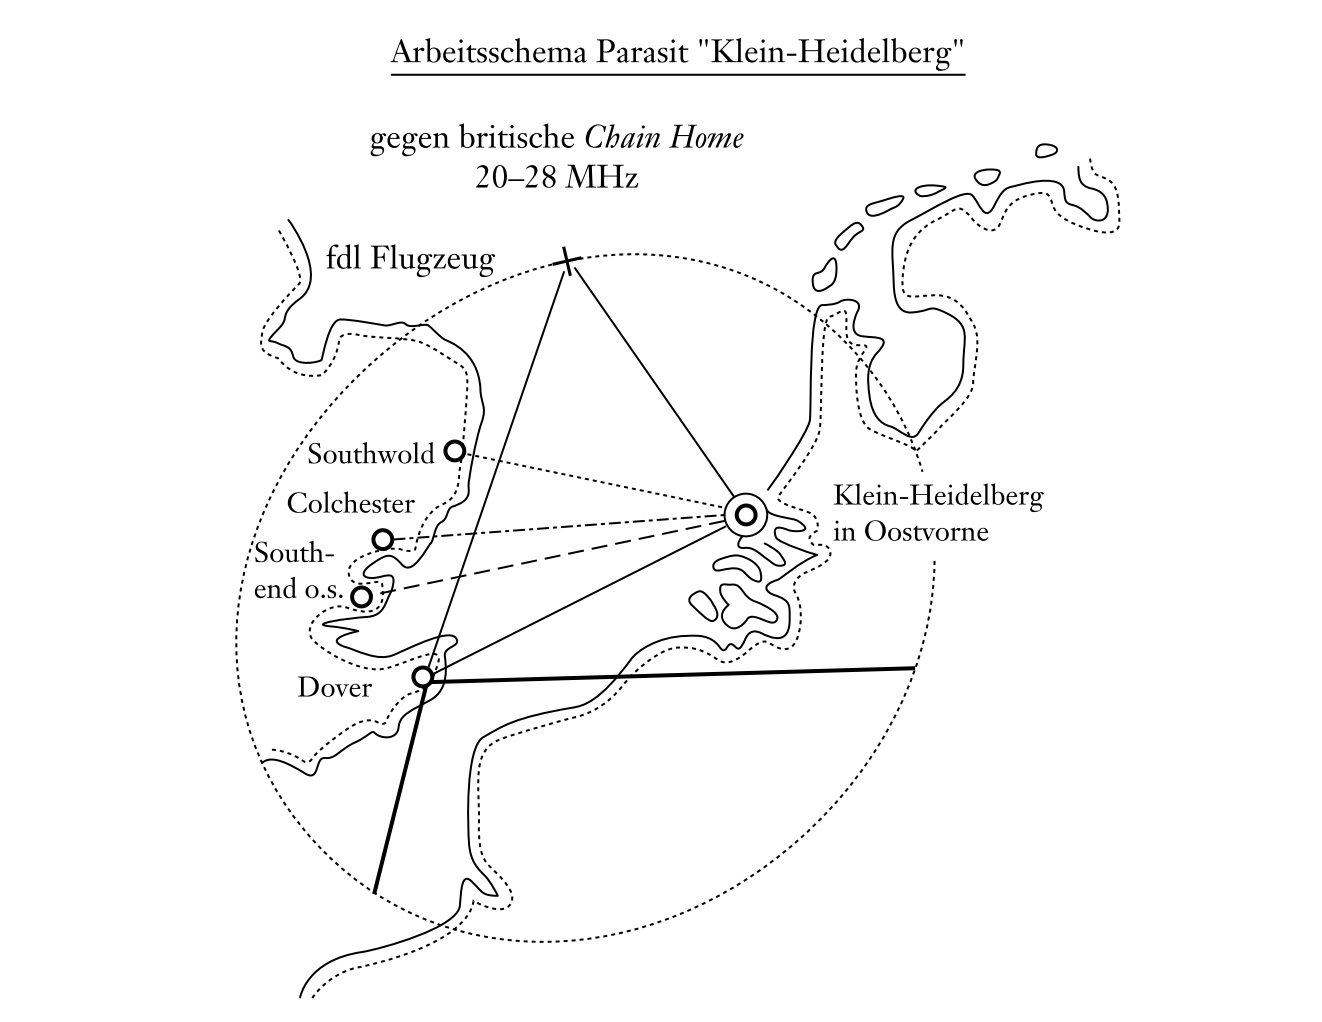
\includegraphics[width=0.85\linewidth]{Figure/KHeid.png}
	\caption{Sketch of the Klein Heidelberg (KH) geometry.}
	\label{fig1:klein}
\end{figure}

After World War II, there has been a lot of extensive research on \ac{PR}. The elimination of a dedicated transmitter requirement and the use of commercially available ready-made components has enabled numerous universities and research institutions to create experimental setups \cite{Colone2023}. Following these developments, Lockheed Martin pioneered the prototype development of the earliest \ac{PR} \ac{FM}-radio broadcasts \cite{Kuschel2010a}, succeeded by further developments from industry and research institutions.

%%%% Definiton of the basic prinicples in Passive \ac{Radar}
\ac{PR} systems are a type of \ac{Radar} that utilize non-cooperative or cooperative illuminators of opportunity, such as commercial broadcasts (\ac{FM}, \ac{DAB},
and \ac{DVB-T/T2}), cellular signals, \ac{WiFi}, and satellite-borne transmitters (\ac{GNSS}, \ac{DVB-S/S2}), to detect and track objects. \ac{PR} systems do not emit any signals but rely on the reflections from targets illuminated by signals from other transmitters(illuminators of opportunity). The principle of \ac{PR}  is based on cross-correlating a signal directly received from the transmitter and signal reflected from the target \cite{Kuschel2010a}. Figure  \ref{fig1:multistatic} illustrates a multi-static \ac{PR} system from \cite{mltistaticRadar}.
%diagram to illustrate a passive \ac{Radar} system.

\begin{figure}[ht!]
	\centering
	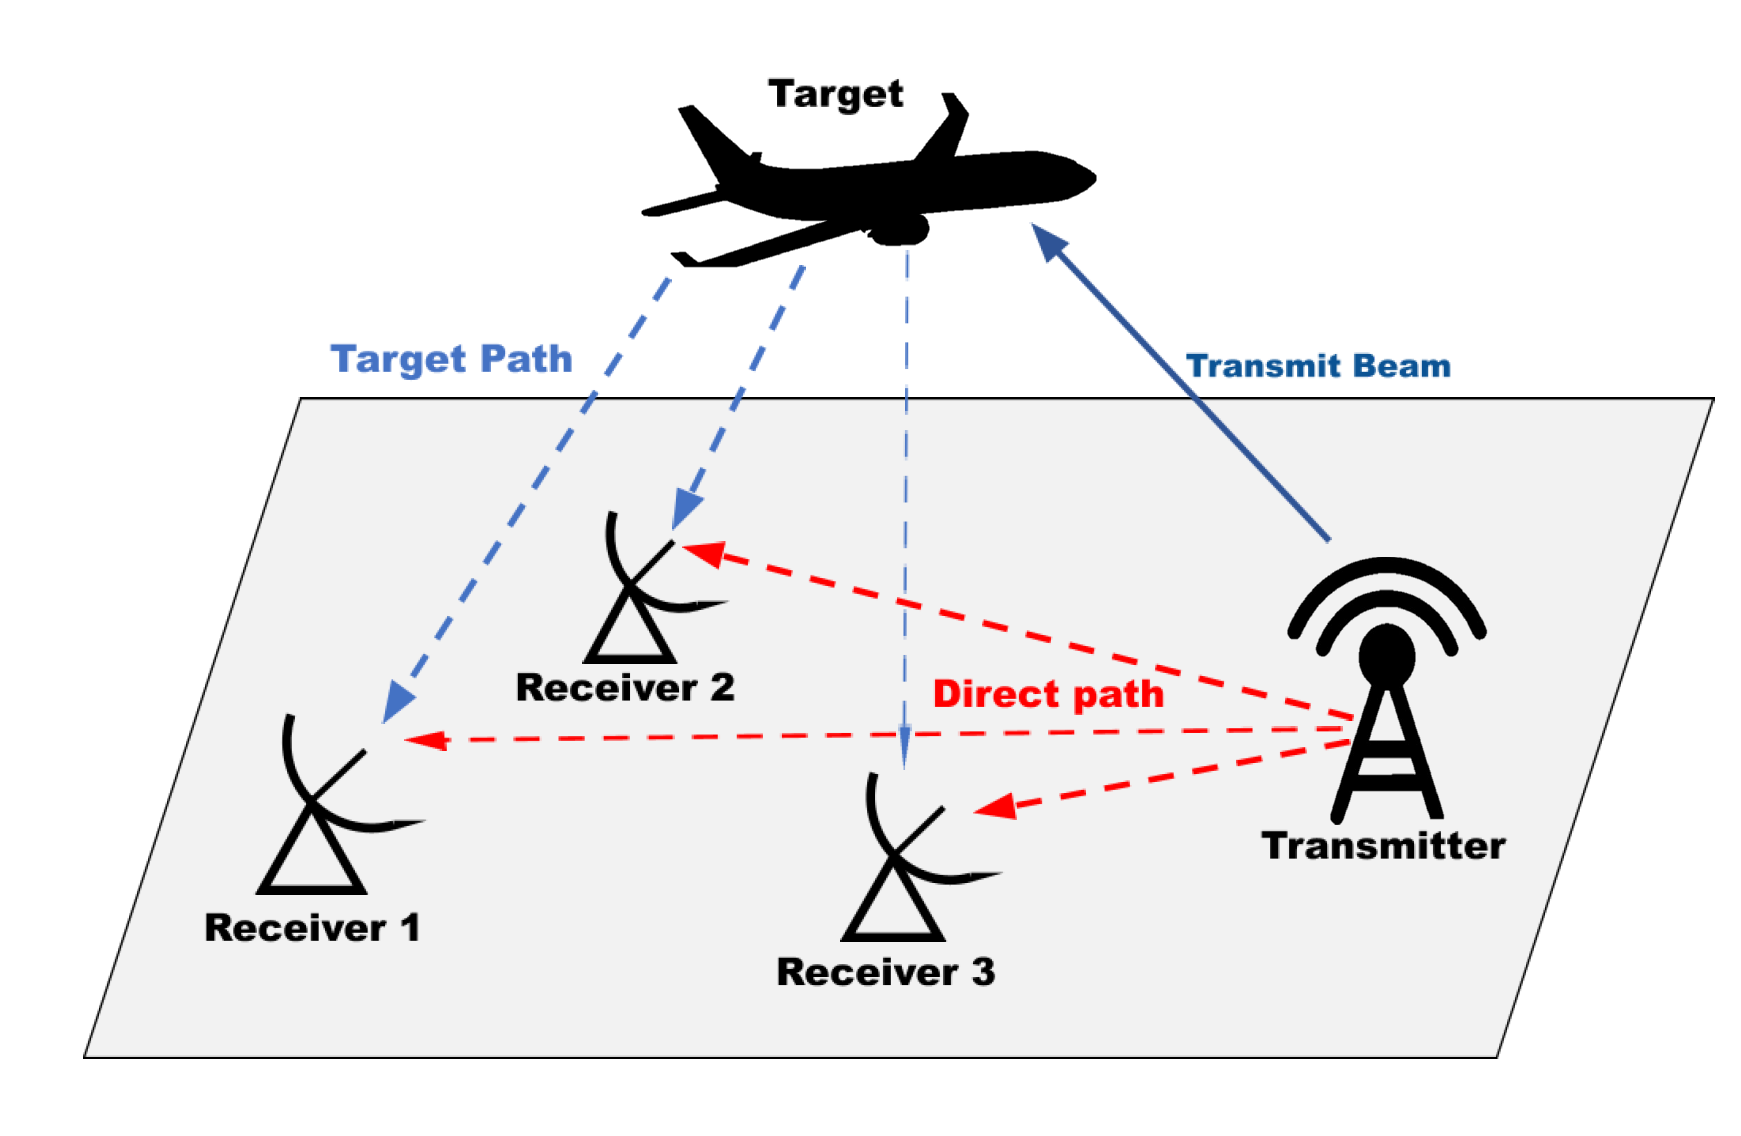
\includegraphics[width=0.9\linewidth]{Figure/Multistatic_Passive_Radar_System.png}
	\caption{Multi-static Passive Radar System with multiple receivers and a single transmitter.}
	\label{fig1:multistatic}
\end{figure}

%%%% Components and architecture 
A typical \ac{PR} system in a multi-static setup, used for target detection and tracking, generally comprising of several key components:

\begin{itemize}
    \item \textbf{Receiving antennas:} 
    \newline
    (Receiver 1, Receiver 2 and Receiver 3)  as observed in Figure \ref{fig1:multistatic}, are antennas used to capture the direct signals from the transmitter and the echo signals reflected from the targets.
    \item \textbf{Illuminator of Opportunity:} 
    \newline
    This component emits the direct signals used for target detection and tracking.
    \item \textbf{Signal Processing Unit:} 
    \newline
    Located at each receiving antenna, these units process the received signals to extract relevant data.
    \item \textbf{Target detection and Tracking:}
    \newline
    Utilizing the outputs from the signal processing units, detection algorithms such as \ac{CFAR} and various tracking algorithms are used in this block to detect and track targets.
\end{itemize}

Figure \ref{fig1:spu} illustrates the signal processing block diagram for an FM radio-based bistatic \ac{Radar}, similar to the one presented in \cite{Howland2005a} and \cite{tong2014}. This diagram demonstrates the typical signal processing stages involved after the signals are received from the antennas.

\begin{figure}[H]
	\centering
	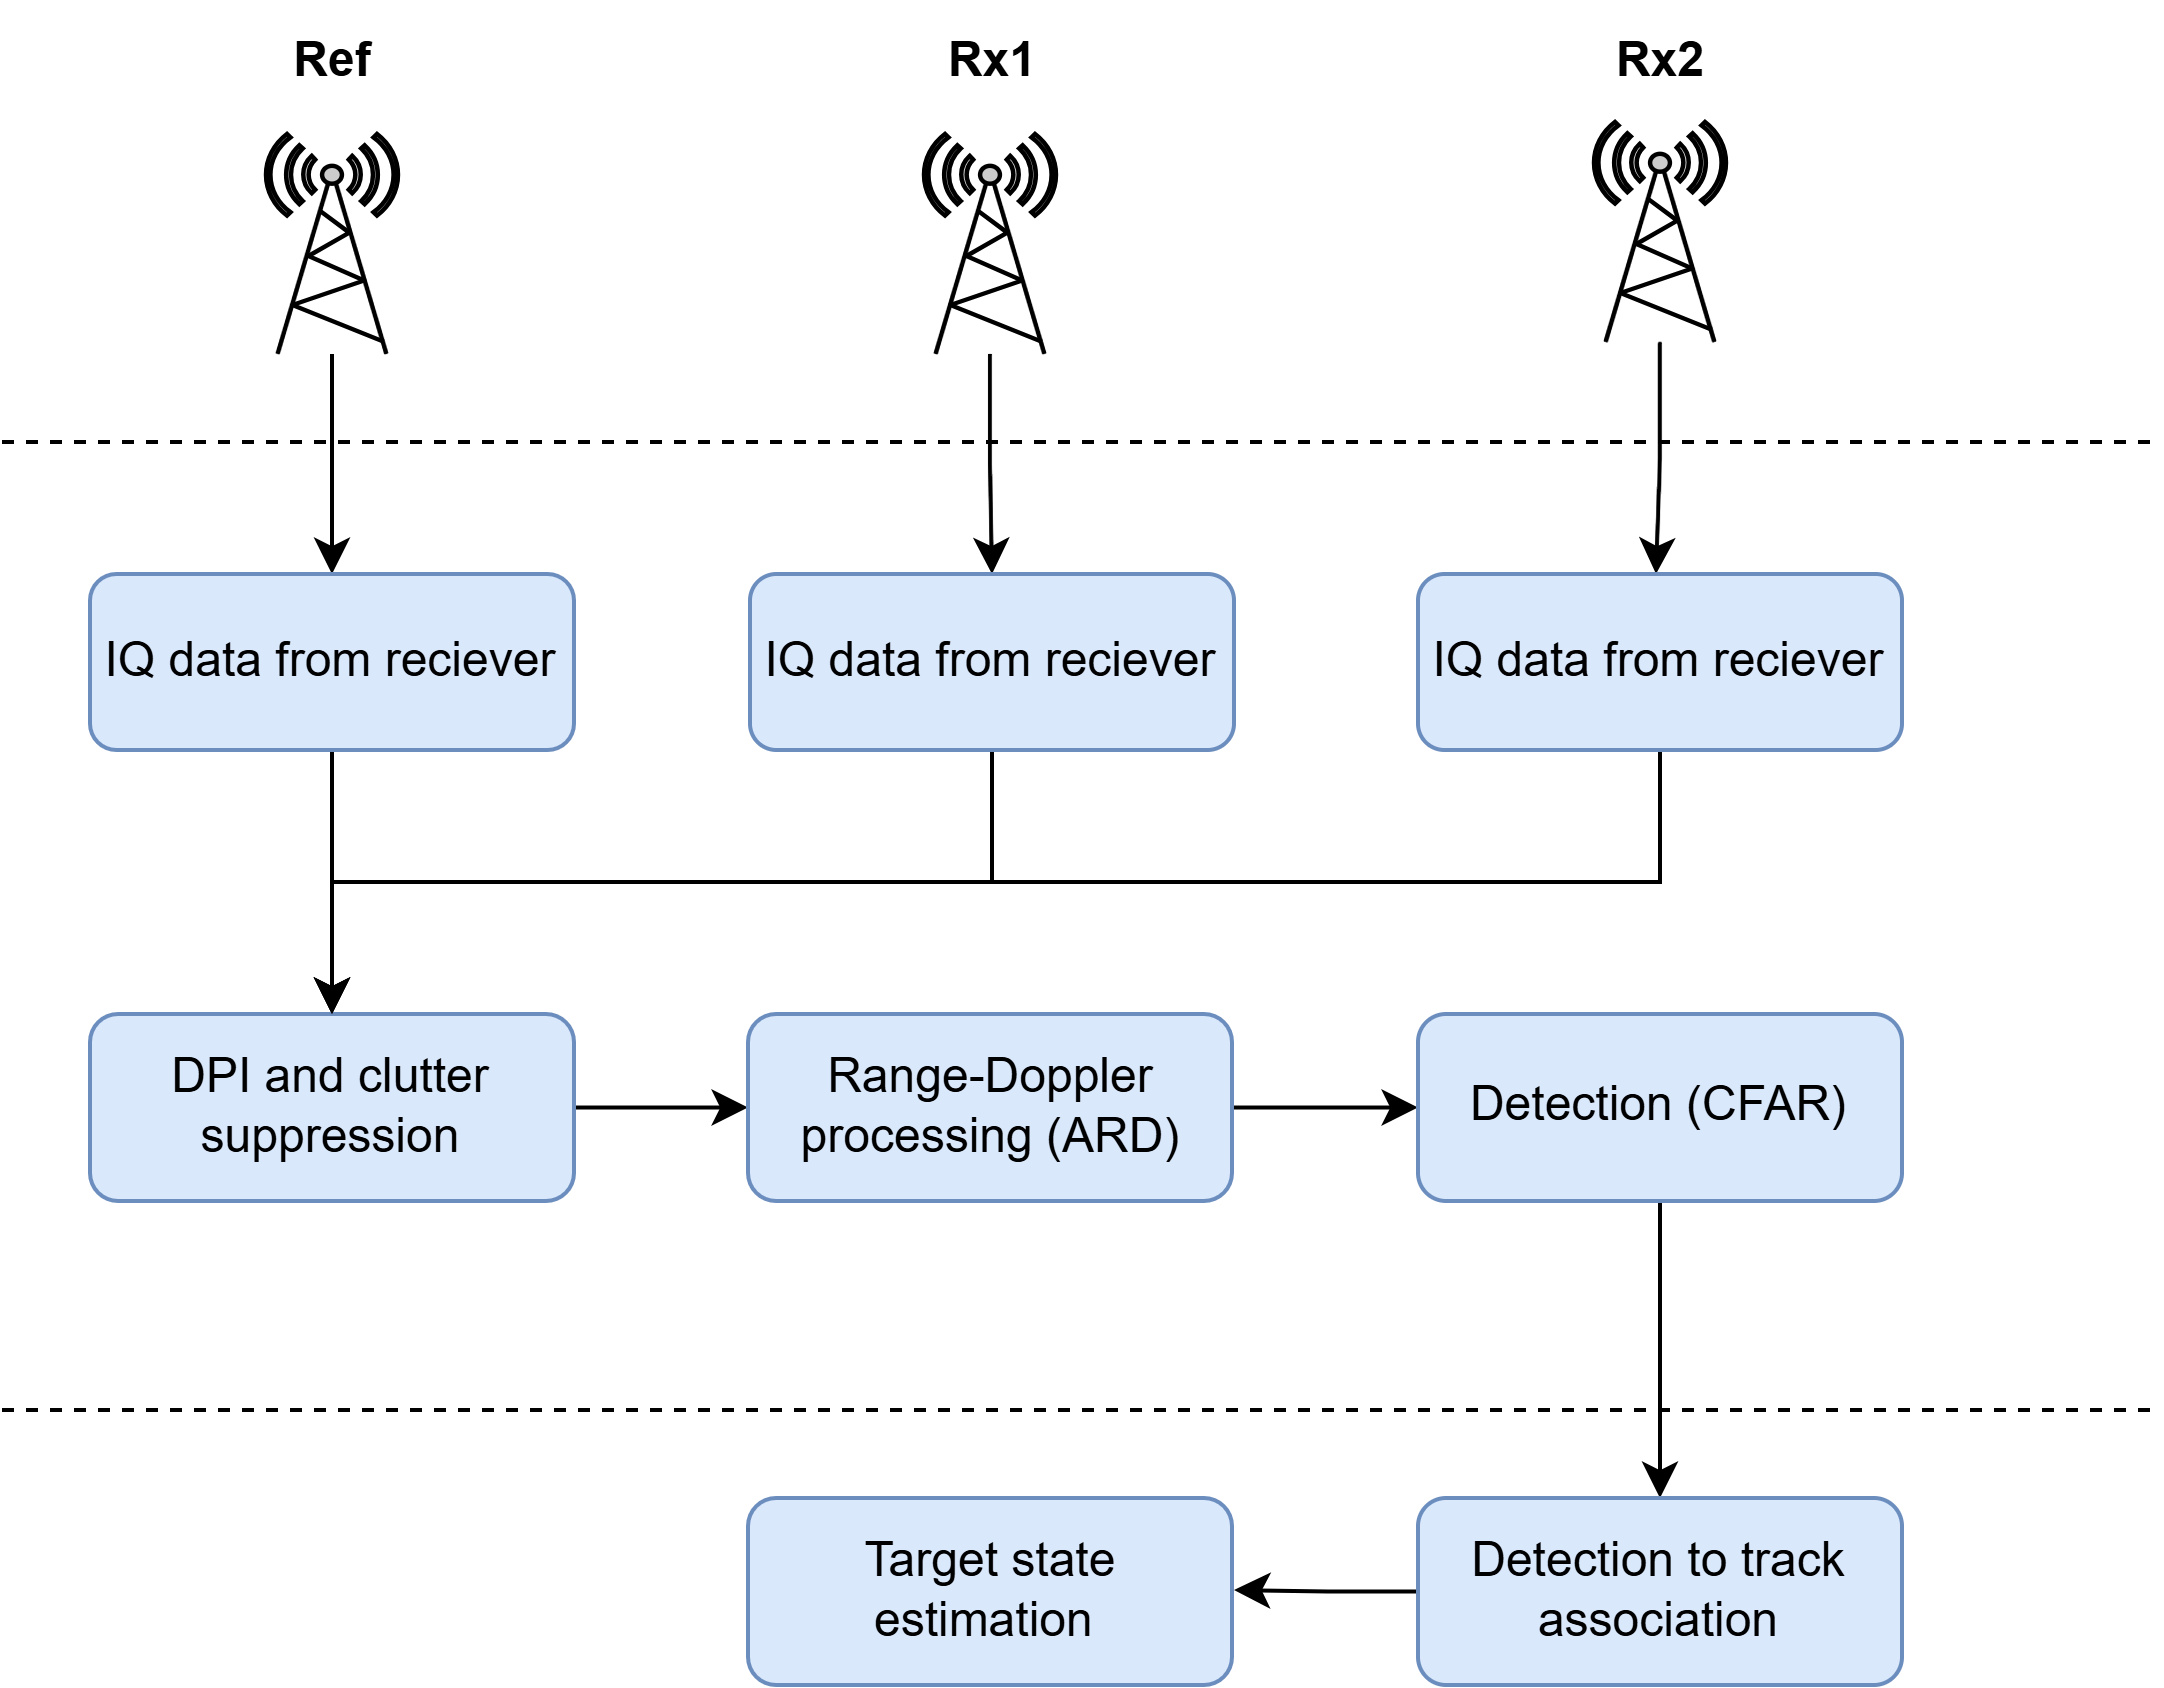
\includegraphics[width=0.9\linewidth]{Figure/fersBistaticRadar.drawio.dsp2.png}
	\caption{Signal Processing Block used for processing signals from the receiving antennas.}
	\label{fig1:spu}
\end{figure}

The general method of evaluating target positions from a bistatic or multi-static \ac{Radar} setup by calculating the difference in range between the target and multiple known locations is known as localization \cite{Friedlander1987}. In \cite{Howland2005a}, the received echo and the reference signal are correlated to compute the relative delay which is related to the bistatic range. The bistatic range is the total distance, measured as the sum of the range from the transmitter to the target and from the target to the receiver. The cross ambiguity function, which represents the correlation between the reference signal and the echo signal as a function of time delay and Doppler frequency shift is then used to calculate the \ac{TDOA} parameters and Doppler shift of the target. The cross ambiguity function \( \chi(\tau, \nu) \) is defined as:
\begin{equation}
\chi(\tau, \nu) = \int_{-\infty}^{\infty} s_T(t) s_R^*(t - \tau) e^{-j2\pi\nu t} \, dt
\label{crossamb}
\end{equation}

where \( s_T(t) \) represents the transmitted (reference) signal, \( s_R(t) \) is the received (echo) signal, \( \tau\) is the time delay, \( \nu \) is the Doppler frequency shift and \( s_R^*(t - \tau) \) is the complex conjugate of the received signal delayed by \( \tau \). Target localization is then achieved by identifying the highest value of correlation on the cross ambiguity function which indicates the time delay and frequency shift where the echo and reference best match \cite{Khalafalla2024}.
%%%% Typical Applications 

\subsection{State Estimation}
%History of state estimation
The history of state estimation dates back to more than 200 years ago when C.F Gauss presented his work on the method of least squares in 1821 and 1823, although Legendre had already investigated it in 1806 followed by Laplace in 1812 who also did an intensive study on problems of estimation\cite{Physics}.
%What is State estimation in Passive \ac{Radar}

The state of a system comprises one or more variables that characterize the status of a system at a given time; for instance, in the case of a moving target like a vehicle, these variables can represent parameters such as position, velocity and acceleration of the target. The problem of state estimation focuses on estimating the state of the system since the true state of the system is typically not directly measurable or known. Instead, observations of the state are made indirectly through measurements which are also affected by noise \cite{Dunik2020}.

In \cite{Levy2008}, the problem of estimation is explored through various methods that differ in design philosophy and metrics used for performance evaluation. This review follows a similar approach, covering the following methods:
\begin{itemize}
    \item Bayesian Estimation methods
    \item Frequentist approach to estimation problems (Classic Estimation)
\end{itemize}
%Bayesian Estimation
In  Bayesian estimation methods, all parameters of the state are treated as random variables, and their probability distribution can be derived either from physical modelling approaches or empirically through extensive data collection from numerous experiments \cite{Levy2008}. The primary objective is to determine the \ac{PDF} of the state $x_k$ given the measurements $z_k$. This \ac{PDF} denoted as $p(x_k \mid z_k)$, represents the conditional probability of the state $x_k$ given the observed measurements $z_k$ where $p(x_k \mid z_k)$ describes the likelihood of the state $x_k$ given the specific measurements $z_k$ \cite{Dunik2020}.

%Frequentist estimation 
In the frequentist approach, all parameters are considered fixed but unknown and are estimated solely based on the observations or measurements. Among such estimators, the \ac{ML} estimator is an optimization approach that determines the values of the unknown parameters that maximize the likelihood of the observed data occurring \cite{Levy2008}. The development of a state estimator relies on a state-space model that represents the physical dynamics of the system \cite{Hasdiana2018}. In the case of a moving object, the model describes the kinematic relationship of the state variables. Additionally, the design of the state estimator also comprises of a measurement model which describes the relationship between the sensory data or measurements and the state of the system. 

In Figure \ref{fig:generic_state_space_model} a generic state space model adapted from \cite{CHEN2} is illustrated to model the stochastic filtering problem. Given the initial density $p(x_o)$, transition density $p(x_t|x_{t-1})$, and likelihood $p(y_t|x_t)$.
The primary goal of filtering is to determine the optimal current state at time $t$ by using all the measurements available up to time $t$ taking into consideration the input data as well. For instance, the Kalman Filter operates as a predictor-corrector algorithm where the predictor models the evolution over time while the corrector updates the estimate based on measurements \cite{Richards2010}.
%State space models
\newline
\begin{figure}[ht!]
	\centering
	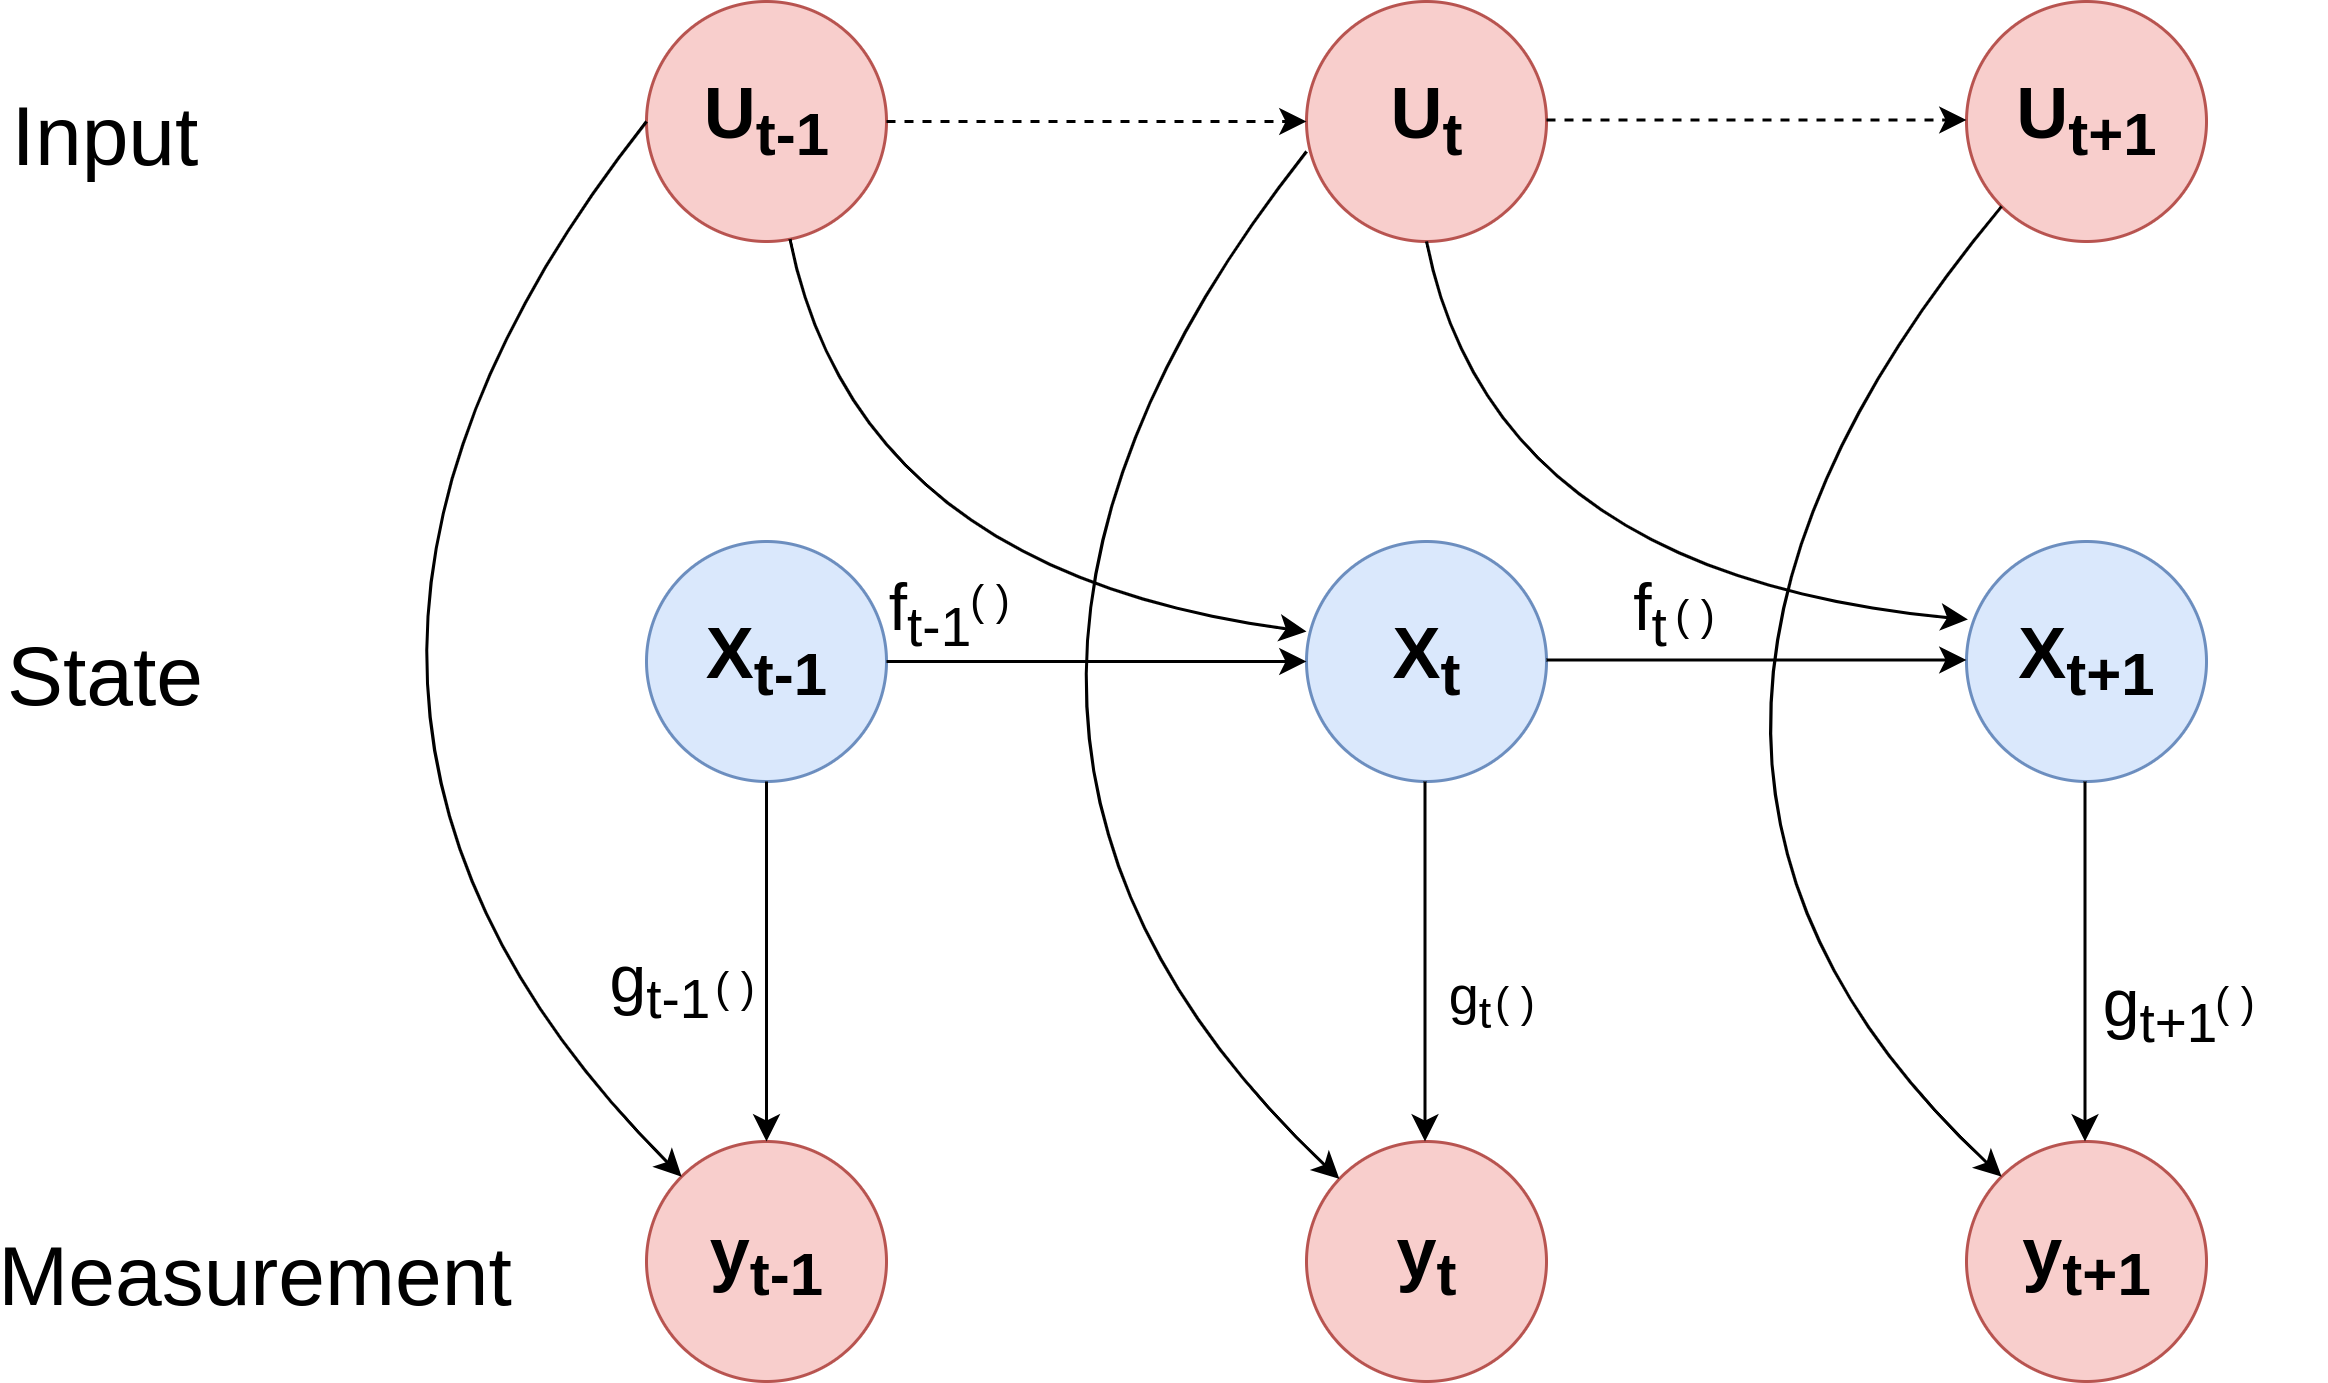
\includegraphics[width=0.75\linewidth]{Figure/genericStateSpace.drawio (1).png}
	\caption{A generic state-space model.}
	\label{fig:generic_state_space_model}
\end{figure}
%Continous vs discrete time

\section{Tracking Filters}
In the introduction, the historical context of \ac{PR} and various estimation methodologies used in estimation theory were explored. This section focuses on tracking filters extensively utilized in \ac{Radar} systems. Specifically, a review of the Kalman Filter and its variants, Particle Filters, Gauss-Newton Filters, Polynomial Filters, and tracking filters based on deep learning is presented.

\subsection{Kalman Filter}
Stochastic filtering emerged in the mid-twentieth century, largely inspired by the groundbreaking contributions of Norbert Wiener, who formulated optimal signal estimation from noisy measurements as a rigorous mathematical optimisation problem. The Wiener filter minimised the mean square error of the estimate using the statistical properties of the signal and noise, and attracted interest among mathematicians, scientists, engineers and computer scientists \cite{CHEN2003}. However, it required the entire measurement history and assumed stationary processes, making it unsuitable for real-time applications, limitations that Kalman would later address through a recursive reformulation of the problem.
%Prior to Kalman's work, Wiener filters required the entire measurement history and assumed stationary processes, making them computationally prohibitive for real-time applications and unsuitable for tracking dynamic targets.In 1960, Rudolf E. Kalman introduced a revolutionary approach that fundamentally changed the landscape of estimation theory \cite{Kalman1960}. The Kalman Filter's key innovation was its \textit{recursive} structure, which required only the previous state estimate and current measurement to compute the optimal estimate—eliminating the need to store or reprocess historical data. This breakthrough enabled real-time implementation on the limited computing resources available in the 1960s.Furthermore, Kalman's state-space formulation allowed the filter to handle \textit{non-stationary} and \textit{time-varying} systems, a critical requirement for tracking maneuvering targets. For linear systems with Gaussian noise, the Kalman Filter is provably optimal in the minimum mean-square error sense, providing both theoretical guarantees and practical performance.
The Kalman Filter and its various adaptations have played a significant role in filter theory for many years. As noted by S. Chen \textit{et al.} \cite{CHEN2}, \textquotedblleft Kalman Filters are widely used in modern engineering and scientific disciplines, including communications, machine learning, neuroscience, economics, finance, and political science, among others\textquotedblright. However of importance to this project, is the use of Kalman Filters in FM \ac{PR}.

%application in Apollo project
The Kalman Filter revolutionized state estimation through its recursive formulation, which enabled real-time computation using only the previous state estimate and current measurement, in contrast to earlier methods like the Wiener filter that required storing and processing entire measurement histories \cite{Andrews2010,schmidt1981}. The Kalman Filter was utilized in the Apollo Project to estimate the spacecraft's position and facilitate complex orbital trajectories. This was particularly crucial for the return journey, where the Apollo Command Module, with its three-member crew, had to re-enter the Earth's atmosphere at an optimal angle. An excessively steep angle would result in the module burning up, while a shallow angle could lead to it bouncing off the atmosphere \cite{Andrews2010}. In 1961, a team led by S.F Schmidt at \ac{NASA} \ac{ARC} implemented the Kalman Filter in digital computer simulations to tackle the circum-lunar navigation challenge and also solved the Apollo guidance and navigation problem using a mainframe computer with a 36-bit floating-point arithmetic \cite{Andrews2010}. This practical implementation demonstrated the filter's capability to handle non-stationary, time-varying dynamics with limited computational resources.

It is well-established that the Kalman Filter has been extensively utilized over the years, spanning from conventional \ac{Radar} tracking domains to now tracking in domains such as Doppler and bistatic range \cite{Joshi2022,Howland2005a}. For instance,  Howland et al.~\cite{Howland2005a}  demonstrated that a four-state Kalman Filter can effectively associate target echoes in the range and Doppler space using FM bistatic \ac{Radar}. Furthermore, in \cite{Joshi2022}, a ship tracking algorithm was proposed which does target tracking in range and Doppler space using range compressed airborne \ac{Radar} data, where a Kalman Filter with \ac{CA} and \ac{CV} motion models are compared to handle target tracking.
%Applications outside \ac{Radar} tracking

Another significant area of research where the Kalman Filter is widely used is visual tracking in computer vision \cite{Gunjal2018, Merven2004}. A method for moving object detection in surveillance systems is demonstrated in \cite{Gunjal2018}, where a target is tracked across video frames by identifying its centre coordinates. The Kalman Filter is used to estimate the location of the moving target from the reference frame to the current frame. Furthermore, N.C. Yang \textit{et al.} \cite{Yang2009} demonstrate the use of Kalman Filtering in video compression to eliminate \textquotedblleft spatial and temporal redundancies in video sequences \textquotedblright. Temporal redundancies are typically addressed through motion compensation techniques, which adjust object displacements from a reference frame to the current frame. In \cite{Yang2009}, a Kalman Filter-based motion estimation algorithm is presented, improving motion estimation in video coding.

%Challenges and Limitations
Although the Kalman Filter is widely recognized for its simplicity, tractability, and robustness \cite{Julier1997a}, it has notable limitations, particularly when dealing with non-linear state dynamics and observation models. Consequently, variants such as the \ac{EKF} and the \ac{UKF} are frequently employed to address these challenges. These variants address the limitations of the standard Kalman Filter, offering better performance in non-linear applications. The variants of the Kalman Filter and other tracking filters are discussed in the subsequent sections of the literature review.

\subsection{Extended Kalman Filter}
The \ac{EKF} is a non-linear adaptation of the Kalman Filter, specifically designed for handling non-linear systems. It follows a similar approach to the Kalman Filter but differs in how it handles the system dynamics. Unlike the standard Kalman Filter, which assumes linear state transition and observation models, the \ac{EKF} extends its applicability to non-linear systems by requiring that these models be differentiable. It achieves this by leveraging the differentiability of the state transition and observation functions, enabling linear approximations through first-order Taylor series expansions\cite{Aditya}. The \ac{EKF} can be viewed as the non-linear version of the Kalman Filter which allows for the linearization of non-linear models about the current estimate. 

For non-linear dynamic systems, the linear Kalman Filter becomes inadequate because it is not possible to define the process or measurement models using the multiplication of vectors and matrices. The \ac{EKF} provides an efficient solution for dealing with non-linear models and has been extensively used in \ac{Radar} for tracking maneuvering targets with non-linear state dynamics. Kim and Bang in \cite{Kim}, also emphasize that the \ac{EKF} is computationally more efficient than other non-linear filtering methods such as point-mass filters and Particle Filters. Furthermore, its widespread use in real-time applications highlights its practical significance where the Kalman Filter falls short.

Key steps for the digital computer simulations at \ac{ARC} for solving the circum-lunar navigation problem led to the development of the \ac{EKF}. Monte-Carlo analyses demonstrated that the non-linearities of the trajectory did not affect the accuracy of the \ac{EKF} for the expected error ranges for the Apollo missions \cite{Andrews2010}. Furthermore, the studies at \ac{ARC} indicated that \ac{EKF} would give comparable accuracies to the weighted least squares estimator while significantly reducing the requirements for onboard computer memory and computation speed \cite{schmidt1981}. However, at that time the \ac{EKF} had not yet been verified to function properly with the available flight computers, a challenge later addressed by the \ac{MIT} laboratory in their subsequent work on the Apollo system.

%Some work done using EKF
Since its initial implementation, the \ac{EKF} has been extensively utilized in applications where the errors from the linear approximations are negligible compared to the measurement errors. A prominent application of the \ac{EKF} is its role in estimating position and velocity in \ac{GNSS} receivers to synchronize the receiver clock with \ac{GPS} \cite{Grewal2006}. Of importance to this research is the application of the \ac{EKF} in \ac{Radar} target tracking, in a study conducted in \cite{Measurements2023b} the \ac{EKF} is implemented to track targets in a \ac{3D} Cartesian space using bistatic range and range rate measurements with a \ac{PBR} system that has no bearing angle information. Furthermore, the \ac{EKF} is demonstrated to be effective in tracking a target using raw measurements of bistatic range and bistatic velocity from a \ac{DVB-T} \ac{PR}, where \ac{EKF}-based tracking is combined with adaptive beamforming techniques for angle estimation \cite{Pasculli2013}.

\subsection{Unscented Kalman Filter}
 The \ac{EKF} as discussed in the previous section, linearizes the non-linear models so that the traditional Kalman Filter can be applied. However, despite the wide usage of the \ac{EKF} as a filtering technique, certain drawbacks such as ease of tuning and implementation in cases where the linearization errors are significant, the filter implementation results in a biased and sub-optimal filter. Recognizing these limitations, Julier and Uhlman developed and demonstrated a novel Unscented Kalman Filter in \cite{Julier1997a} as an improvement over the \ac{EKF} where some of the practical well-known drawbacks of the \ac{EKF} noted in \cite{Julier1997a} are:
\begin{itemize}
    \item \textquotedblleft Linearisation can lead to significant instability in filters if the assumption of local linearity is violated\textquotedblright, as noted by S.J. Julier in \cite{Julier1997a}.
    \item Computing the Jacobian matrices is often complex in many applications, posing major challenges during implementation.
\end{itemize}
In \cite{Julier1997a}, the analytical superiority of the \ac{UKF} over the \ac{EKF} was demonstrated. The \ac{UKF} operates on the principle that a discretely sampled set of points can effectively characterize both the mean and covariance. These sample points accurately represent the true mean and covariance of a Gaussian random variable. As noted by Z. Cai and D. Zhao \cite{Cai2006},  \textquotedblleft When the sample points are passed through the true non-linear system, they effectively capture the updated mean and covariance accurately to the 3rd order (Taylor series expansion) for any non-linear function compared to the 1st order (Taylor series expansion) linearisation in \ac{EKF}\textquotedblright.

The \ac{UKF} uses the unscented transform where deterministic sample points account for non-linearities of the system \cite{Yin2021}. Although the \ac{UKF} achieves the accuracy of a third-order Taylor series expansion, it does so without the computational complexity of calculating the Jacobian matrix. According to A. Asif  \textit{et al.} \cite{Measurements2023b}, \textquotedblleft there is no general formula for calculating the values of the sigma points; therefore, it is crucial to make accurate approximations of the parameters based on the specific estimation problem\textquotedblright.

%Applications of the EKF
In most applications requiring high accuracy state estimation such as autonomous navigation, the \ac{UKF} is usually used over the \ac{EKF} \cite{Costanzi2017,Grewal2006,Costanzi2019}. In \cite{Costanzi2017}, the \ac{UKF} is compared to the \ac{EKF} where the \ac{UKF} is illustrated to be effective in bearing-only target localization even when the positions of the sensors are unknown. In another study \cite{Ortenzi2009}, the \ac{UKF} is compared to the \ac{PF}, showing that the \ac{UKF} offers comparable performance to the \ac{PF} with reduced computational load and ease of algorithm setup in a bistatic \ac{Radar} environment where a non-cooperative \ac{FM} radio station is used as a transmitter of opportunity.
%limitations of the UKF

Similar to the \ac{EKF}, the \ac{UKF} is limited to models with Gaussian noise assumptions \cite{Konatowski2017}. For state estimation in scenarios where models do not adhere to Gaussian assumptions or involve non-Gaussian noise, Particle Filters offer a viable alternative. In the next section, a review of the literature on Particle Filters is presented.
%Gaussian assumptions
%
\subsection{Particle Filters}
The Particle Filter is a type of sequential Monte Carlo method developed initially for target tracking by N.J. Gordon \textit{et al.}  \cite{NJGordon}. In contrast to the Kalman Filter and its variants (\ac{EKF},\ac{UKF}), the \ac{PF} as highlighted by \cite{MFeroz} operates without the strict assumptions of linearity and Gaussianity. This flexibility allows the \ac{PF} to effectively handle non-Gaussian noise distributions and accommodate non-linearities in both the measurements and dynamics of the target.

Monte Carlo methods use repeated random sampling to generate their results. They begin by defining a domain of possible inputs and then generate random input samples from a posterior distribution over this domain. These samples are used to perform computations, producing output samples, which are then analyzed to infer the output probability distribution \cite{Hoffman}. There are various versions of the \ac{PF} throughout literature, in \cite{Hoffman} different state-space Particle Filters based on different resampling methods are discussed namely:
\begin{itemize}
    \item Bootstrap \ac{PF}
    \item Auxillary \ac{PF}
    \item \ac{MCMC} \ac{PF}
    \item Linearised \ac{PF}s
\end{itemize}
In \cite{Arulampalam2007} variants of the \ac{PF} are introduced within the generic framework of the \ac{SIS} and these variants are compared, with some showing better performance in specific applications. Alternative architectures to the generic \ac{PF}s are also proposed for \ac{PR} target tracking \cite{Zhao2013,Tobias2008}.

The superiority of the \ac{PF} over the non-linear Kalman Filters is demonstrated in certain cases. For example, \cite{Abdoul-Moaty2014} shows that the \ac{PF} is more effective as a predictor in a multi-static \ac{Radar} environment, where it successfully corrects its path despite noisy measurements. Additionally, an improvement to the \ac{PHD}-based \ac{PF} for target detection in \ac{PR} is introduced in \cite{Tobias2008}, which enhances reliability and significantly reduces the number of particles required for tracking.

\ac{PF}s have limitations, including their dependence on sample size. A small particle set may not accurately approximate the true state and increasing the sample size, while addressing this issue, also raises computational requirements \cite{Zhong2016}. Particle degeneracy, where many particles have negligible weights, further complicates the situation and is typically addressed through resampling methods. New algorithms proposed in \cite{Zhong2016} tackle particle impoverishment and sampling dependency, resulting in improved tracking performance for non-linear single-variable estimation problems.

In the next section, the Gauss-Newton filters are reviewed, which are also applicable to non-linear dynamics and observation models.

\subsection{Gauss Newton Filter}
%What are Gauss-Newton Filters
Gauss invented the method of least squares and the Gaussian \ac{PDF} at the beginning of the nineteenth century \cite{Zhichao2018}. This was a significant breakthrough in estimation theory. By combining this with the differential calculus developed by Newton, Gauss created the Gauss-Newton algorithm.
%Limitations and Disadvantages
In 1958, Swerling \cite{Zhichao2018} found that the non-recursive Gauss-Newton algorithm was unsuitable for tracking targets such as satellites due to the limited computational capacity of computers at that time. He proposed a new recursive algorithm later known as the Swerling filter. With today's vast processing capacities, the Gauss-Newton filter has become feasible for application in some non-linear systems.

The Gauss-Newton filter allows for long prediction times, enabling data updates without intervals. Its finite memory length can be varied, which allows for adaptability, making it suitable for estimating targets with high dynamics. In this case, the filter acts like a sliding window, focusing on the most recent 
observations \cite{nmorris2013}. 

\begin{comment}
        
Table \ref{gnf_key_attributes} adapted from \cite{improvedGauss} highlights some of the key attributes of the Gauss-Newton filters compared to the linear Kalman Filter.
\newline
\begin{table}[ht]
    \centering
    \renewcommand{\arraystretch}{1.3} % Adjust the row height
    \begin{tabular}{|p{6cm}|p{3cm}|p{3cm}|} % Adjust column widths
    \hline
    \textbf{Key Attributes}                 & \textbf{GNF}   & \textbf{Kalman Filter} \\ \hline
    Data update frequency                      & flexible timestamps & Constant interval      \\ \hline
    Suitable for highly changing dynamics & Yes            & No                     \\ \hline
    Requires prior initialization                          & No             & Yes                    \\ \hline
    Handles noise in tracking    & Yes            & Yes                    \\ \hline
    Recursive computation                   & No             & Yes                    \\ \hline
    \end{tabular}
    \caption{Key differences between Gauss-Newton Filters and Kalman Filters.}
    \label{gnf_key_attributes}
\end{table}
\newline
\end{comment}


While Gauss-Newton filters provide superior numerical results, robustness, and effectiveness in tracking maneuvering targets, \cite{nmorris2013} highlights that they can suffer from slow convergence or, in some cases, fail to converge. This has necessitated research into enhancements for this filter. Some advancements to the Gauss-Newton filter include merging the \ac{LMA} into the Gauss-Newton filter. In \cite{roaldje}, the iterative version of the Gauss-Newton filter with memory introduced by Norman Morrison in \cite{NmorrisHIll} is adapted to the \ac{LMA} to ensure consistent convergence. It is further demonstrated that the adapted algorithm is robust to random disturbances and non-linear trajectories, where it is used to track targets in Cartesian coordinates with bearing, Doppler, range, and elevation observations \cite{roaldje}. In another study \cite{Morrison}, the Gauss-Newton filter was shown to be able to track aircraft using bearing and Doppler information from a \ac{PR} system.
%Introduce RGNF 

The \ac{GNF}, while robust and effective, it demands substantial computational resources \cite{improvedGauss}. In \cite{costa}, two hardware designs on \ac{FPGA} co-processors are implemented to enhance the performance of the \ac{GNF}. The recursive form of the \ac{GNF}, namely the \ac{RGNF}, was presented to reduce the amount of computational memory required, which was previously recognized as a major limitation for the \ac{GNF} \cite{Inggs1}.

\subsection{Recursive Gauss-Newton Filter}
The Recursive Gauss Newton Filter(RGNF) is an extension to the \ac{GNF}, recently reorganised into a recursive format to track targets in a computationally efficient manner. In \cite{improvedGauss}, the recursive form of the \ac{GNF} is obtained with zero memory to demonstrate the application of the compact recursive form of the \ac{GNF} to non-linear process dynamics and non-linear observation schemes. Subsequent development of the \ac{RGNF} by Nadjiasngar \cite{Inggs1} involves adapting the filter to the \ac{LMA} method similarly to the study in \cite{roaldje} for the \ac{GNF}.
%Some of the applications of the RGNF

The \ac{RGNF} is chosen for tracking targets in a multi-static \ac{Radar} environment that exploits FM radio signals using Doppler-only measurements \cite{De2015}. This study demonstrated the filter's effectiveness in tracking targets with real measurement data collected from at least three receiver sites. Another study \cite{Boyer2012} showed that the \ac{RGNF} significantly outperforms the Kalman Filter and \ac{PF}, resulting in better tracking accuracy and lower computational load for scenarios where the state transition and observation models are linear for tracking in the Doppler and range domain.

\subsection{Polynomial Filters}
Polynomial filters function by fitting a polynomial to a sequence of noisy observations using the least squares method, as introduced in Morrison's book "Introduction to Sequential Smoothing and Prediction" \cite{NmorrisHIll}. These filters are based on Laguerre and Legendre polynomials. Filters based on Legendre polynomials, which have a uniform weight function, are known as \ac{EMP} filters. In contrast, filters based on Laguerre polynomials, which have an exponentially decaying weight function, are called \ac{FMP} filters. The basic structures of the one-step predictor \ac{FMP} and \ac{EMP} filters are similar, allowing for easy switching between the two by changing the weights, this adaptability gives birth to the Composite EMP/FMP filter, which utilizes both types of filters \cite{nmorris2013}.
\newline
\newline
\begin{figure}[ht!]
	\centering
	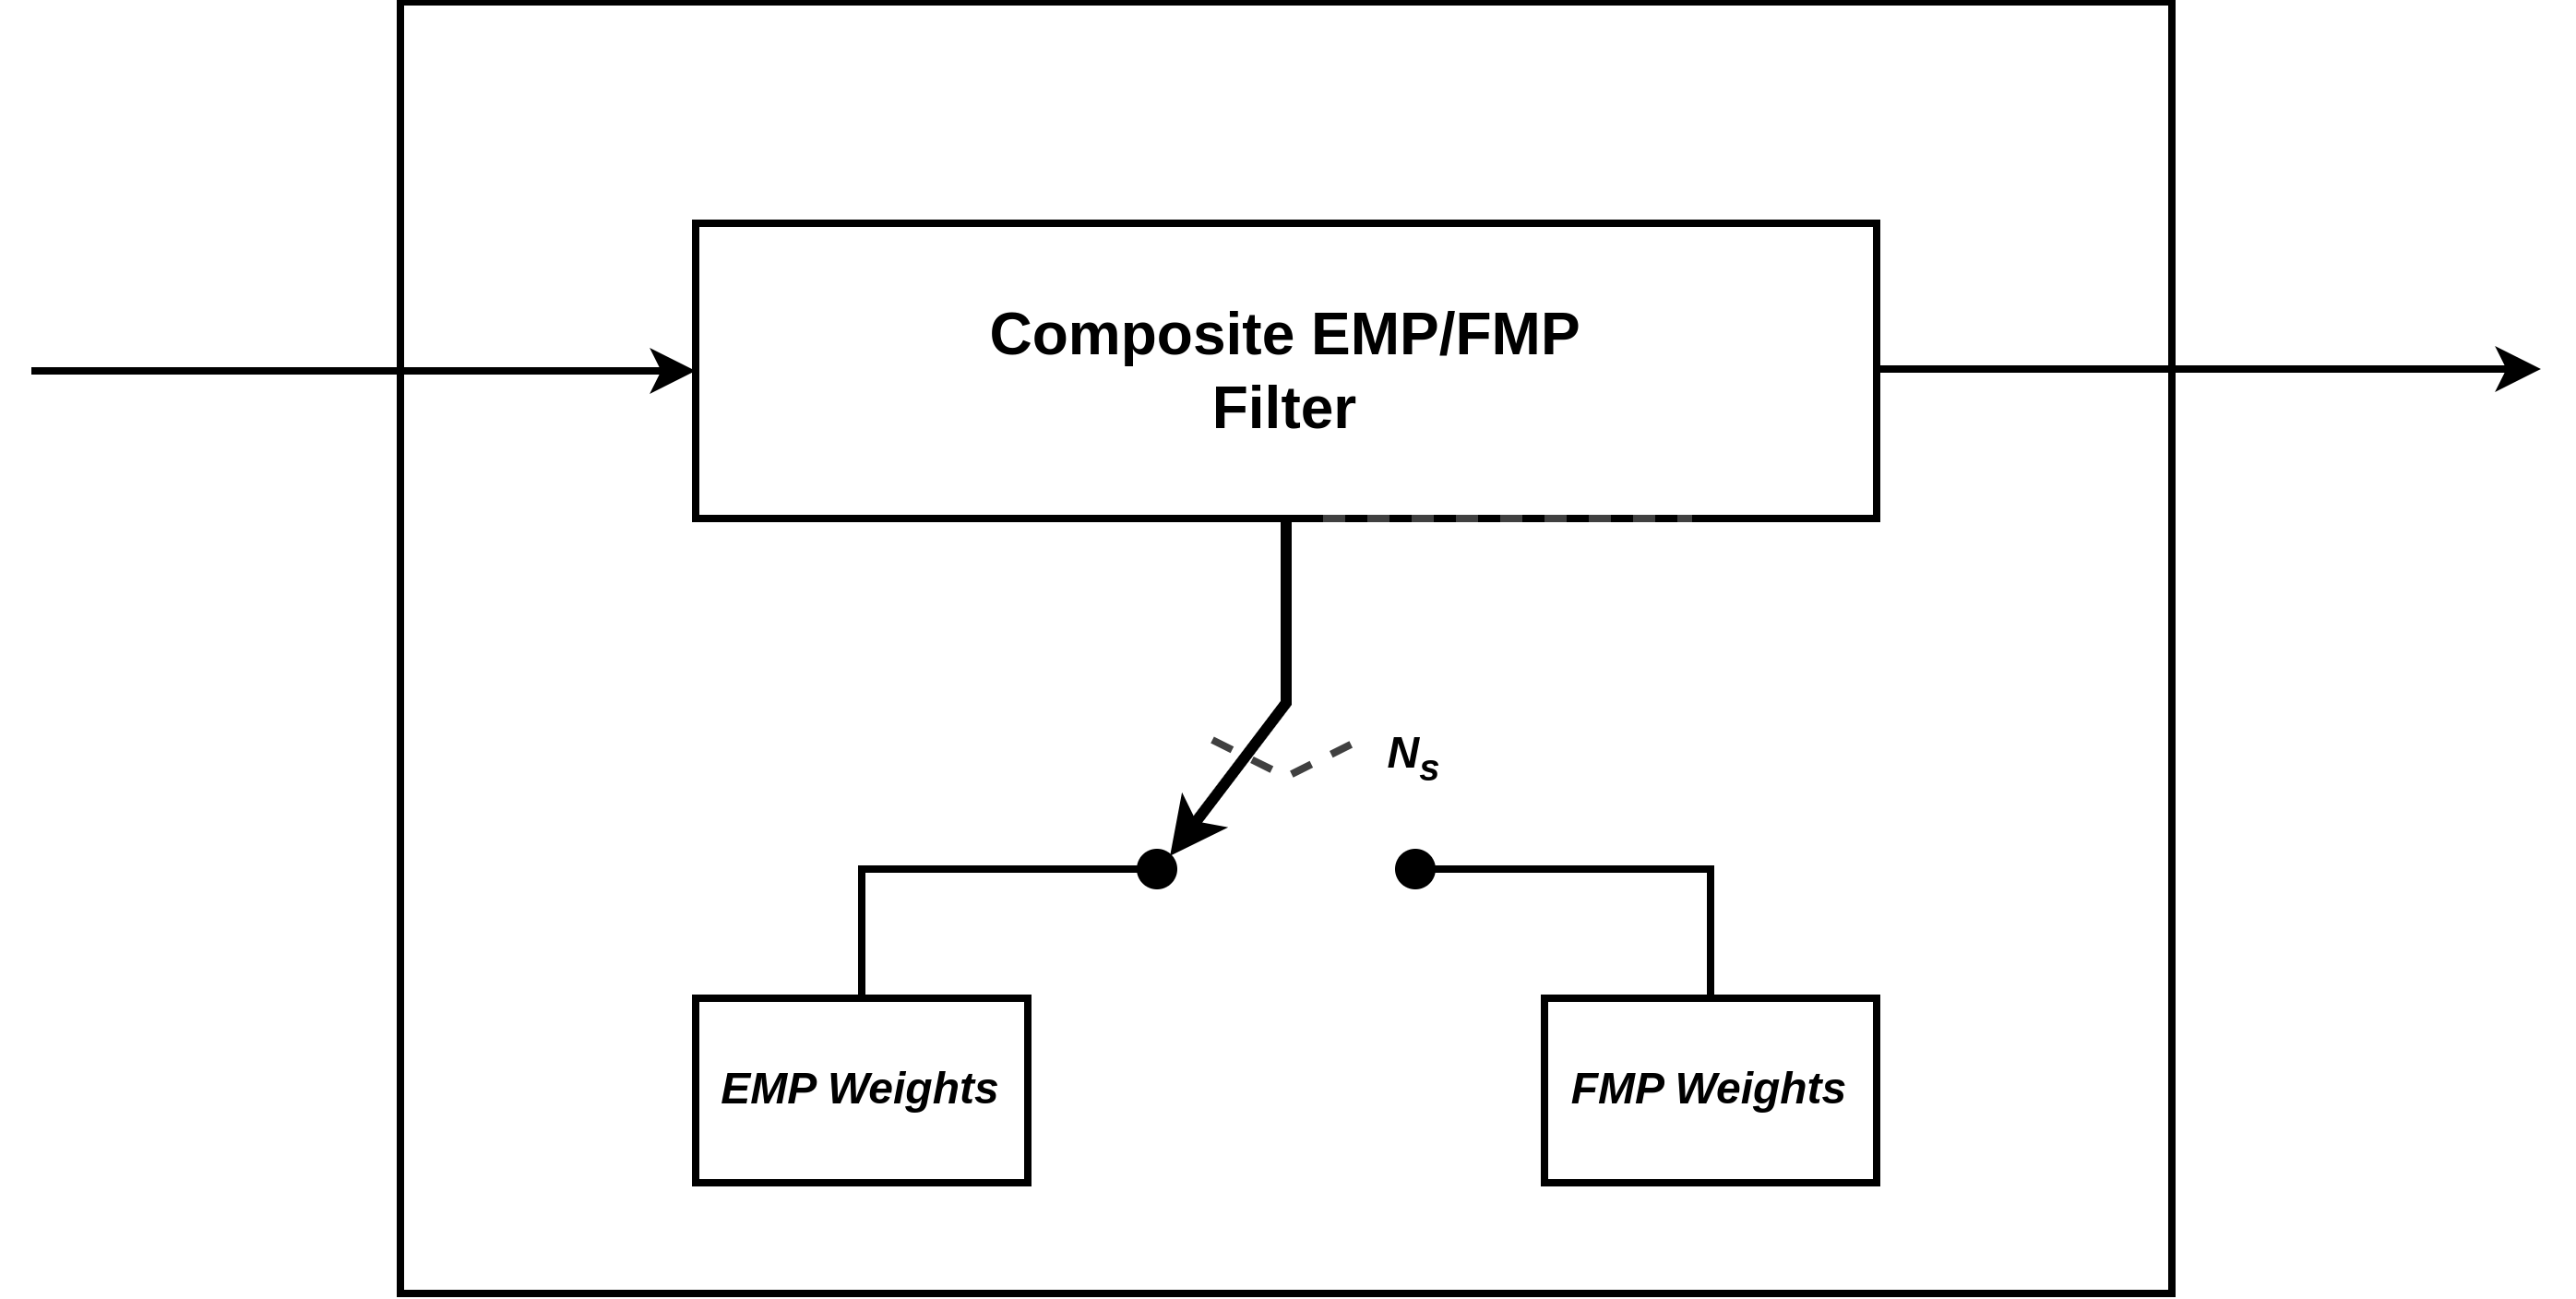
\includegraphics[width=0.85\linewidth]{Figure/compositeP (1).png}
	\caption{Composite EMP/FMP filter.}
	\label{fig:compositeEMP}
\end{figure}
\newline
The Composite Polynomial Filter leverages both the advantages and disadvantages of the \ac{EMP} and \ac{FMP} filters. The \ac{EMP} filter initiates itself automatically but is limited in tracking targets for prolonged periods and can track changing trajectories effectively, whereas the \ac{FMP} filter requires an external initialization but can track targets for longer durations \cite{Boyer2012}. In the Composite filter, as observed in Figure \ref{fig:compositeEMP} adapted from \cite{nmorris2013}, the weights are switched when the filter covariance matrices are equal, which occurs at a transitional sample number  \(N_s\) \cite{nmorris2013}.
\newline 
\newline
According to Norman Morrison's book on Gauss-Newton and Polynomial Filters \cite{nmorris2013}, the composite \ac{EMP}/\ac{FMP} filters, as well as the individual \ac{EMP} and \ac{FMP} filters, can be used for a variety of applications, including but not limited to:
\begin{itemize}
    \item The composite \ac{EMP}/\ac{FMP} filter can be used as a high-data-rate tracker for pedestal control in \ac{Radar} systems and can also be used as a pre-filter for Gauss-Newton or Kalman Filters.
    \item As described in \cite{nmorris2013}, \textquotedblleft the current-estimate \ac{EMP} filter can function as a self-initializing algorithm to initialize Gauss-Newton or Kalman Filters\textquotedblright.
    \item The \ac{EMP} filter can be used to fit a polynomial curve to a sequence of noisy observations using the method of least squares.
\end{itemize}
There are a few studies based on using the composite \ac{EMP}/\ac{FMP} filter for target tracking purposes \cite{Lu2020, Nadjiasngar2011a}. A study in \cite{Lusilao-Zodi2010} \textquotedblleft focuses on the estimation of round-trip time for the transport layer in \ac{TCP} for multimedia applications\textquotedblright. In this study, the filter is used to predict future round-trip times from previously recorded values, demonstrating that the filter can effectively capture model dynamics and non-linearities with less memory space and fast execution times. The composite \ac{EMP}/\ac{FMP} filter is shown to be effective as a pre-filter to the \ac{UKF} for tracking a maneuvering target in a complex scenario \cite{Lu2020}. Furthermore, in \cite{Nadjiasngar2011a}, a \ac{PDA} filter based on the composite \ac{EMP}/\ac{FMP} filter is proposed, achieving comparable results to the Kalman Filter. 

Recent advancements in deep learning have paved the way for new approaches to tracking filters, and in the next segment, a review of some of these methods will be presented.


\subsection{Deep Learning - Based Tracking Filters}
Current filters can generally address the filtering problem for tracking targets. However, as noted by Cui \textit{et al.} \cite{cui2022}, there are still several challenges, such as an excessive number of filtering variants and forms, and a lack of tight coupling with the target motion model. In recent years, there has been a significant trend towards the use of deep learning approaches for target tracking, especially in visual tracking applications \cite{Yang2017,Supreeth2018,Bouzenada2007}. For this review, tracking filters not based on \ac{NN} will be referred to as traditional filters.
\newline
\newline
%What are Neural Networks and categories for Tracking
Throughout the literature, \ac{NN}s are employed in target tracking filters in several distinct ways, as highlighted in  \cite{cui2022}. Some common trends in research for target tracking with \ac{NN}s include: Firstly, integrating \ac{NN}s with traditional filters without altering their structure to enhance performance \cite{Duh2004}; Secondly, using \ac{NN}s to replace specific modules and estimate parameters within traditional filters without changing their overall frameworks \cite{Xu2023}; And lastly, using \ac{NN}s to completely remodel the filtering function, thereby breaking away from the traditional filter's composition and framework \cite{cui2022}. \ac{NN}s are machine-learning models designed to mimic the functionality of biological neural networks in the brain. In terms of computational graphs, traditional filters primarily use linear operations such as division, subtraction, addition, and multiplication, along with nonlinear operations and delayed feedback structures, all of which can be implemented within neural network architectures \cite{cui2022}.
%Network Topologies-
%Some work using neural networks

In \cite{cui2022}, various \ac{NN} topologies are implemented to create a unified model that mimics the operations of both the Kalman Filter and the $\alpha-\beta$ filter. This unified model utilizes \ac{RNN}, \ac{FNN}, and attention mechanisms. The study demonstrates that the non-linear operations of the Kalman Filter can be represented using a \ac{FNN}, where the delayed feedback can be modelled as an \ac{RNN}, and the filter gain can be captured by attention mechanisms.

In another study, a Deep Neural Network-based tracking filter is developed for tracking maneuvering targets  \cite{Liu2019}. This model is trained offline using abundant trajectory data from existing maneuvering targets and has demonstrated superior performance compared to state-of-the-art algorithms for maneuvering target tracking. Furthermore, in \cite{Xu2023}, a Generalized Regression Neural Network (GRNN) is combined with a Kalman Filter to investigate its effectiveness in non-linear approximation from target measurements to target positions. This study highlights the potential of integrating \ac{NN} techniques with traditional filtering methods to enhance tracking performance.

%\subsection{Adaptive Tracking Filters}

\section{Multi-Target Tracking}
In the previous section, various tracking filters used in \ac{Radar} applications were reviewed and were shown to be fundamental for estimating the state of a single target. However, it is essential to examine how these filters fit into the more complex scenario of \ac{MTT}. \ac{MTT} focuses on developing algorithms and techniques for tracking multiple targets simultaneously within an environment under observation. In \ac{Radar} target tracking, \ac{MTT} aims to jointly estimate the number of targets, their states, or trajectories from noisy measurements \cite{Vo2015}. \ac{MTT} involves techniques such as observation to track association and track maintenance.

%\subsection{Target Tracking}
\subsection{Data Association Techniques}
The initial step in multi-target tracking is to accurately interpret sensor data, ensuring that each measured data point corresponds to the correct tracked object. This process typically involves gating and assignment techniques. Several widely used techniques for associating observations with existing tracks are reviewed.
\newline
\newline
\begin{figure}[htb!]
	\centering
    \includesvg[width=1\linewidth]{Figure/MTTDiagram.drawio.svg}
	\caption{Basic elements of a conventional MTT.}
	\label{fig:MTT_Diagram}
\end{figure}
\newline
Figure \ref{fig:MTT_Diagram} illustrates the typical process of updating a track at each update, as described in \cite{Blackman}. The highlighted observation-to-track association block is unique to \ac{MTT}, addressing the combinatorial assignment of M measurements to N tracks. The observation-to-track association technique focuses on the assignment of observations to tracks. Gating, defined as the process of eliminating observations that are unlikely to belong to a track based on a specific gating method, reduces computation for the data association step \cite{Konstantinova2003}. Data association illustrated as observation-to-track association in Figure \ref{fig:MTT_Diagram}, occurs after the gating process. This step is crucial for densely spaced targets, where additional logic is needed to determine the most likely target for each track.

In an environment with clutter, some of the measurements being fed into the tracker may not be due to real targets but rather to clutter or false alarms. This causes ambiguities in associating the existing target tracks with the measurements at every update. Such ambiguities can result in poor target tracking and overwhelm computational resources. As a result, there has been extensive research in the area of \ac{MTT} to resolve the problem \cite{Blackman}. One of the most used methods of data association in \ac{MTT} is the \ac{GNN} approach \cite{Liu2022,Shi2013,Konstantinova2003}.

\subsubsection{Global Nearest Neighbor}
The \ac{GNN} is an extension of the Nearest Neighbor association that functions by searching for unique joint associations of measurements from targets to tracks, maximizing likelihood or minimizing distance \cite{Stevens2011}. One of the advantages of the \ac{GNN} is its simplicity in implementation, as well as its low memory and computational resource usage because it only uses the most likely hypothesis for data association \cite{Shi2013}. A modified version of the \ac{GNN} is used to perform data associations in the presence of sensor bias based on the relative distance or topology of the sensor observations \cite{Shi2013}. A study in \cite{Saputra2023} utilizes the \ac{GNN} as a \ac{MTT} due to its fast execution time for application in aircraft tracking for Ground-Controlled Interception \ac{Radar}. In another study, the \ac{GNN} is used to effectively associate inter-frame detections from a Video Synthetic Aperture \ac{Radar} image sequence. The \ac{GNN} filter is prominent in the space of \ac{MTT}; however, there are certain drawbacks to it despite its efficiency. In \cite{Smith2019}, it is noted that it is prone to losing tracks and having poor performance in cases where targets are closely spaced. Misassignment or track loss can be severe for the filtering process, causing the filter to slowly converge or fail to converge.

\subsubsection{Joint Probabilistic Data Association }
%% Probability data Assoiication filter
The \ac{JPDA} is derived from the \ac{PDA}, which was introduced in the 1970s \cite{Bar-Shalom1974}. Unlike the \ac{PDA}, which considers each measurement-target association independently, the \ac{JPDA} computes the association probabilities jointly across all targets. This means that at each update, the \ac{JPDA} uses all measurements and weighs them according to their respective association probabilities \cite{OnderBozdogan2016a}. It is also mentioned in \cite{Blackman}, that the \ac{JPDA}  outperforms the \ac{GNN} in heavily cluttered multi-target environments. For this reason, the \ac{JPDA} algorithm is widely used in \ac{MTT} research. In \cite{Khalil2016} it is demonstrated that the \ac{JPDA} used in conjunction with the Constant Turn Rate Model \ac{UKF} can provide accurate state estimates of a target while minimizing track loss. The study in \cite{Braca2012}, shows the usage of \ac{JPDA} and \ac{UKF} applied to target tracks generated by two \ac{HFSW} \ac{Radar}s and \ac{AIS} data. Despite the widespread adoption of the \ac{JPDA}, the \ac{JPDA} has limitations due to its combinatorial nature, requiring substantial computational resources. To address this problem \ac{RFS} methods are usually implemented.

\subsubsection{Random Finite Set Methods}
As previously discussed, an \ac{MTT} scenario involves a collection of individual target states and measurements, in contrast to single target systems, where the state and measurement of the target at time \( k \) are two vectors with possibly different dimensions. These multi-target states and measurements can vary over time as targets appear and disappear. An \ac{RFS} is a set of finite-set-valued random variables and consists of a random number of points \cite{Jerrelind2020}. An \ac{RFS} instance \( X = \{x_1, \ldots, x_n\} \) consists of random, distinct, and unordered points, making \ac{RFS} a natural representation for multi-target states and measurements \cite{Vo2005}. In \cite{Jerrelind2020}, the \ac{MTT} problem is formulated as a filtering problem with a multi-target state space \( \mathcal{F}(\mathcal{X}) \) and observation space \( \mathcal{F}(\mathcal{Y}) \), where the sets of targets and measurements are denoted as \( X_k \) and \( Y_k \) respectively \cite{Jerrelind2020}.
\newline
\begin{equation}
    X_k = \{ x_{k,1}, \ldots, x_{k,M_k} \} \in \mathcal{F}(\mathcal{X}) 
\end{equation}
\begin{equation}
    Y_k = \{ y_{k,1}, \ldots, y_{k,N_k} \} \in \mathcal{F}(\mathcal{Y}) 
\end{equation}
\newline
Here, \( M_k \) represents the number of targets and \( N_k \) denotes the number of measurements at time \( k \). Among the various methods based on the \ac{RFS} framework is the \ac{PHD} filter \cite{Clark2005,PHAMNAMTRUNG2007,Vo2005}. The \ac{PHD} filter is an algorithm for \ac{MTT} that recursively estimates both the number and states of multiple targets based on a set of observations \cite{Prihoda2019}. Between 1993 and 1995, in several unpublished manuscripts, Stein \textit{et al.} introduced the concept of \ac{PHS}. This concept involves a probability distribution graph that, when integrated over a target space region, yields the expected number of targets within that region \cite{Mahler2000}. This idea laid the groundwork for the \ac{PHD} filter, which represents the expected value of a random track set and, when integrated over a state space region, determines the precise random number of targets in that region.

A study in \cite{Guldogan2014} addresses the problem of \ac{MTT} in a bistatic \ac{Radar} setup from sensors measuring the Doppler shift. The \ac{PHD} filter and two of its variants are also compared: the \ac{GM-PHD}, introduced in \cite{Vo2006}, which assumes targets follow a linear Gaussian dynamical model with linear Gaussian measurements, and where survival and detection probabilities are state-independent; and the \ac{SMC-PHD}, proposed in \cite{Vo2005}, which offers a more flexible approach compared to the Gaussian Mixture \ac{PHD}, accommodating a broader range of scenarios. It was found that both variants can track multiple targets successfully using Doppler measurements only, with the \ac{GM-PHD} being more effective and easier to implement than the \ac{SMC-PHD}. 

Another variant of the \ac{PHD}, the \ac{CPHD}, is explored in \cite{Ozkan2011} for tracking multiple ground vehicles using acoustic sensor arrays, where the \ac{CPHD} is shown to perform better than the \ac{PHD}. While \ac{RFS} methods are effective for addressing \ac{MTT} problems, the \ac{PHD} filter has a major drawback in terms of computational efficiency \cite{Prihoda2019}, however the \ac{PHD} variants have proven to be robust and more efficient in addressing these issues. Another advantage of \ac{PHD} filters is that they model the birth and death of targets in the observation space, where other data association techniques such as \ac{GNN} and \ac{JPDA} require additional logic for managing the trajectories of targets during the tracking process. Various methods of track management are discussed in the track management section of the review.

\subsection{Track Management}
Track management, also known as track maintenance, is a critical component of the target tracking process. It involves several key functions:
\begin{itemize}
    \item \textbf{Track Initiation}:
    \newline
    This involves assigning a detection to a new track when it is not associated with an existing track. Once a track is initiated, it is considered tentative until further validation.
    
    \item \textbf{Track Confirmation}:
    \newline
    This process verifies the validity of a detected target. It typically involves logic for determining the status of the track based on additional observations.
    
    \item \textbf{Track Deletion}:
    \newline
    This involves removing a track when it is no longer deemed valid. A track may be deleted if the target is lost if it is determined to be a false alarm, or if it has not been updated within a specified time frame.
\end{itemize}
One common approach in track management is the M-out-of-N logic, which is valued for its simplicity \cite{Boyer2012, Kim}. According to this logic, a track is confirmed if there are \(M\) validated detections out of the last \(N\) samples. Conversely, a track is terminated if there have been no valid detections for \(M\) out of the last \(N\) samples. Additionally, unassociated measurements can be used to create new tracks \cite{Braca2012}. For instance, in \cite{Kim2013}, the M-out-of-N logic was applied to a multiple target tracking problem for a \ac{FMCW} \ac{Radar}. This method was used to evaluate the quality of both confirmed and tentative tracks, ensuring that tracks with a low probability of loss were maintained even in the presence of clutter.

Other track management techniques include methods based on track score tests, such as the \ac{SPRT}, Bayesian sequential tests, and batch processing techniques \cite{Blanding2009, Blackman}. \ac{SPRT}-based methods create tentative tracks from detections that are not initially correlated with existing targets. These tracks remain provisional until a sufficient number of observations have been collected to make a statistically reliable judgement. The decision to confirm or terminate a track is based on comparing the likelihood of observations under two hypotheses: a true target hypothesis versus a false alarm hypothesis \cite{Blanding2009, Kajenski2011}. A track is confirmed if its score meets or exceeds a specified threshold; otherwise, it is terminated if the score falls below this threshold.

Bayesian sequential tests, similar to \ac{SPRT}, use Bayesian methods to recursively update the posterior probabilities of various hypotheses. Batch techniques, such as the Hough Transform \cite{Leung1996}, process detections over multiple frames collectively \cite{Blanding2009}. The Hough Transform has been shown to offer long track lifetimes, low false data association rates, and short computational times \cite{Leung1996}.

Despite advancements in track management techniques, the M-out-of-N method remains popular for its simplicity and efficiency. Additionally, in \cite{Khalil2016a} combining the M-out-of-N technique with \ac{JPDA} has been shown to provide accurate estimates of target positions and velocities in automotive \ac{Radar} applications.

\section{Performance Evaluation of Tracking Filters }
In the preceding subsections, various tracking filter algorithms and techniques used in \ac{MTT} have been reviewed. Evaluating the performance of these tracking algorithms is also crucial to determine their efficiency, robustness, and accuracy. When ground truth data is available, metrics such as \ac{RMSE} and \ac{NEES} are frequently used to evaluate the accuracy of the tacking filter estimations through Monte Carlo simulations \cite{Ding, Omar2012a, Inggs1, Nadjiasngar2011a}. Additionally, the Cramér-Rao Lower Bound (CRLB) and its variants, including the \ac{PCRLB} and the \ac{CCRLB}, are also commonly employed performance measures \cite{Junler2020, Nadjiasngar2012, Bauermeister2016}. However, there has been limited research on the use of statistical methods, such as likelihood ratios, for comparing filter estimates with ground truth. Another performance metric that has been used widely to evaluate tracking filter performance in some studies is the processing or computational time \cite{Salih2011,Konstantinova2003}. This is important because tracking algorithms usually have real-time processing constraints.

\subsection{Root-Mean Squared Error}
The \ac{RMSE} quantifies how accurately the target tracking filter matches the true target's path and is usually used when ground truth data is available for validation. Typically, this validation is performed through a significant number of Monte Carlo simulations. For instance, in \cite{Konovalov2016}, the \ac{UKF} provides estimates in Cartesian 3D coordinates from passive \ac{Radar} measurements (bistatic Range and bistatic velocity). The \ac{RMSE} for 1000 individual trials is demonstrated in this study. In another study, the \ac{RMSE} is used as a metric to evaluate the performance of the \ac{RGNF} to compare its performance to the \ac{GNF}. Both the position \ac{RMSE} and velocity \ac{RMSE} are computed through 250 Monte Carlo simulations \cite{Inggs1}.

\subsection{Normalized Estimation Error Squared}
The problem of motion modelling in the range and Doppler domain is examined in \cite{Li2021}, where the \ac{NEES} is utilized to assess the consistency of tracking filters. The \ac{NEES} considers estimation errors, and filter covariance matrices. When NEES values fall within an acceptable range at a given confidence level, the filter is deemed consistent. In another study \cite{ZhenDing2010}, various non-linear filters such as the \ac{UKF}, \ac{EKF}, and Converted Measurement \ac{EKF} are compared using simulated datasets and real recordings from a \ac{ATC} \ac{Radar} experiment dataset and a \ac{HFSW} \ac{Radar} where the filters demonstrated consistency when evaluated using the NEES metric.

\subsection{Cramer-Rao Lower Bound}
The \ac{CRLB} is also widely used to evaluate filters, providing a theoretical minimum bound for the variance(square of precision) of an unbiased estimator \cite{Richards2010}. In \cite{Nadjiasngar2012}, the \ac{CRLB} is also used as a metric for evaluating the performance of a \ac{RGNF} for Doppler-only tracking applications. In \cite{Li2021} it was also found when using the \ac{PCRLB}, the proposed estimation in range and Doppler is close to the theoretical lower bound.

\subsection{Processing Time}
In \cite{Salih2011}, Kalman and \ac{PF} are investigated for \ac{3D} visual tracking, with a quantitative comparison of computational time and accuracy. The computational time per frame is considered, which is the elapsed time from image acquisition to displaying tracking results. Similarly, \cite{Li2021} examines motion modelling and compares the average run-time of various filters against a baseline \ac{UKF}'s run-time.

\subsection{Log-Likelihood}
Another important metric for comparing filter estimations against ground truth, considering the filter's innovation matrix, is the Likelihood function. Unlike probability, which measures the chance of data occurring given a model, Likelihood measures how well a model explains given data. In filtering, the Likelihood function assesses how well the filter's predictions fits actual observations, considering tracking filter innovations and residuals. Often the Likelihood is used as a ratio, known as the Likelihood Ratio Test \cite{Turnbull1978}. Due to its mathematical complexity, the log-likelihood is commonly used instead of the likelihood \cite{Grewal2006}.


\section{Tracking in the Bistatic Range-Doppler Domain}

Numerous studies have explored tracking targets in the bistatic range and bistatic Doppler domains due to extensive research on \ac{PR} and target tracking \cite{Measurements2023b,Li2021,Nadjiasngar2012,De2015,Kim2018}. \ac{PR} measurements offer advantages such as high Doppler resolution, enabling precise radial velocity measurements of targets \cite{De2015}. In some studies, tracking is performed in \ac{3D} Cartesian coordinates to determine the location and velocities of targets, utilizing non-linear observation-to-state dynamics mapping and non-linear filters \cite{De2015,Measurements2023b}. Other studies conduct state estimation directly in the bistatic range and Doppler domain, where measurements are in the same domain, exploring various motion models like constant velocity and constant acceleration \cite{Howland2005a,Kim2018,Li2021}. Additionally, in \cite{Herman2002} the Kalman Filter and the \ac{PF} have been used to track and classify targets using an \ac{FM} passive air surveillance \ac{Radar}, with target estimation performed in the Cartesian coordinate system based on bistatic measurements.

\section{Conclusions}
This section reviews several studies relevant to this research, offering an overview of existing work in the field and highlighting gaps within the current literature. It is evident that a substantial amount of research has been conducted on tracking filters for the purposes of target tracking in \ac{Radar}. As observed from the literature and outlined in the motivation section, there is a need for research focused on tracking commercial aircraft in the bistatic range and Doppler domain. This research aims to design and implement multiple tracking filters for this purpose and compare them using a statistical benchmark.

From the literature discussed, the following topics will be addressed in the subsequent chapters of this dissertation:
\newline
\begin{itemize}
    \item \textbf{Tracking Filters}:
        \newline
        The Kalman Filter is well-known for providing optimal results for linear dynamics and linear observation schemes, making it a strong candidate for the tracking problem considered and serving as a benchmark for other filters. The \ac{UKF} is also considered due to its comparable performance to the other filters, as demonstrated in various studies. Although most of the literature uses the \ac{UKF} for non-linear filtering, it will be applied in a linear context in this case. Another filter to be considered is the \ac{PF}, mainly due to its ability to operate without assumptions of Gaussianity in the observations, its demonstrated superiority over the Kalman Filter in certain cases, and its difference in structural composition to the Kalman Filters. Lastly, the Recursive Gauss-Newton filter is considered, which has proved to be more efficient and optimal in \ac{PR} applications.
    \item \textbf{Method of Data Association}:
        \newline
        The \ac{GNN} is considered due to its ease of implementation and lower computational requirements compared to other data association techniques discussed in the review, such as \ac{JPDA} and \ac{RFS} methods. Additionally, its ability to integrate with various tracking filters, as highlighted in numerous studies, is advantageous.
    \item  \textbf{Track Management}:
        \newline
        The track management method discussed and implemented is the M-out-of-N logic, which has been demonstrated to be efficient in most of the literature.
    \item  \textbf{Performance Evaluation Metric}:
        \newline
        Processing time is considered due to it being an important metric for the target tracking problem, ensuring that the tracking filters compared meet the real-time constraints of the \ac{Radar} tracking system. The log-likelihood will also be used as the performance metric to evaluate the state estimates from the filters compared to the ground truth or measurements.
\end{itemize}
%%%%%%%%%%%%%%%%%%%%%%%%%%%%%%'%

%----------------------------------------------------------------------------------------
%	Section 3
%----------------------------------------------------------------------------------------
\newpage
\chapter{Theory Development}
\section{Introduction}
In the previous chapter, various estimation techniques applied to \ac{Radar} target tracking were reviewed. This chapter establishes the theoretical foundation for the tracking filters developed in this research. Section 3.2 introduces the mathematical foundations of estimation techniques, paving the way for a detailed discussion of the Kalman Filter and the \ac{UKF} in Section 3.3. Section 3.4 discusses the theory behind the \ac{RGNF}, including a thorough derivation and application of its equations. The theory of \ac{PF} is addressed in Section 3.5, beginning with an overview of the fundamental concepts underpinning \ac{PF} theory. Furthermore, Section 3.6 discusses adaptive filtering techniques. Lastly, Section 3.7 introduces the log-likelihood as a statistical benchmark for evaluating the tracking filters.

\section{Target State Estimation Theory}
\ac{Radar} tracking systems are mostly used to measure and estimate the state of the target, which can be the target's range,  elevation angle, azimuth angle, velocity or Doppler frequency, amongst other target parameters. Continuous usage and tracking of these parameters enables the system to estimate their future values. According to Richards \textit{et.al} \cite{Richards2010}, target tracking can be separated into two parts: \textit{a)  Data association for assigning measurements to tracks} and \textit{b) Target estimation with tracking filters}.
\newline
\newline
Measurement-to-track data association involves the assignment and matching of an observation to a corresponding track or the creation of a new track if the detection is from a newly found target, where a track is defined as a collection of values for a single target's state at a specific point in time. In \ac{Radar} or navigation systems, measurements are values that can be extracted from sensors or \ac{Radar} maps such as \ac{CFAR} or range and Doppler maps that have information about the state of the target. The process of measurement-to-track data association can become even more complex due to closely spaced targets, target maneuvers and \ac{Radar} with low resolution, which all make it difficult to classify target measurements and assign them to correct tracks.
\newline
\newline
Track filtering refers to the estimation of a target's trajectory, including its position, velocity, and acceleration amongst other parameters, based on noisy measurements such as range, elevation, and bearing that have been associated with a track \cite{Richards2010}. The estimate of the trajectory from the tracking filter has an uncertainty associated with it that is characterized by the co-variance of the estimate. The predicted position and velocity are then used to estimate the next observation. Figure \ref{fig1:multi-target} illustrates the vital purpose of target tracking in \ac{Radar} systems. In target tracking, a track may denote the position, velocity, or other parameters representing an entity perceived in the environment, while a target is an actual object in the environment that the \ac{Radar} is intended to track. In \cite{Richards2010} it is noted that ``the number of tracks maintained by a \ac{Radar} tracking system can be greater (extra) or fewer (missed) than the actual number of targets''. In a perfect scenario, the number of tracks should match the number of targets. In this section, the fundamentals of single target tracking with a \ac{Radar} are addressed.

In this chapter, the fundamentals of Kinematic State Estimation (track filtering), focusing on two main approaches to filtering algorithms are discussed. The first approach uses deterministic estimation that assumes a perfect model for the target's motion, where the track error covariance approaches zero as more data is processed. In contrast, the second approach uses stochastic state estimation, assuming an imperfect model for the target's motion. In stochastic state estimation, the target's motion model incorporates a random process, and the covariance of the track does not approach zero as more data is processed \cite{Richards2010}.

\begin{figure}[H]
	\centering
	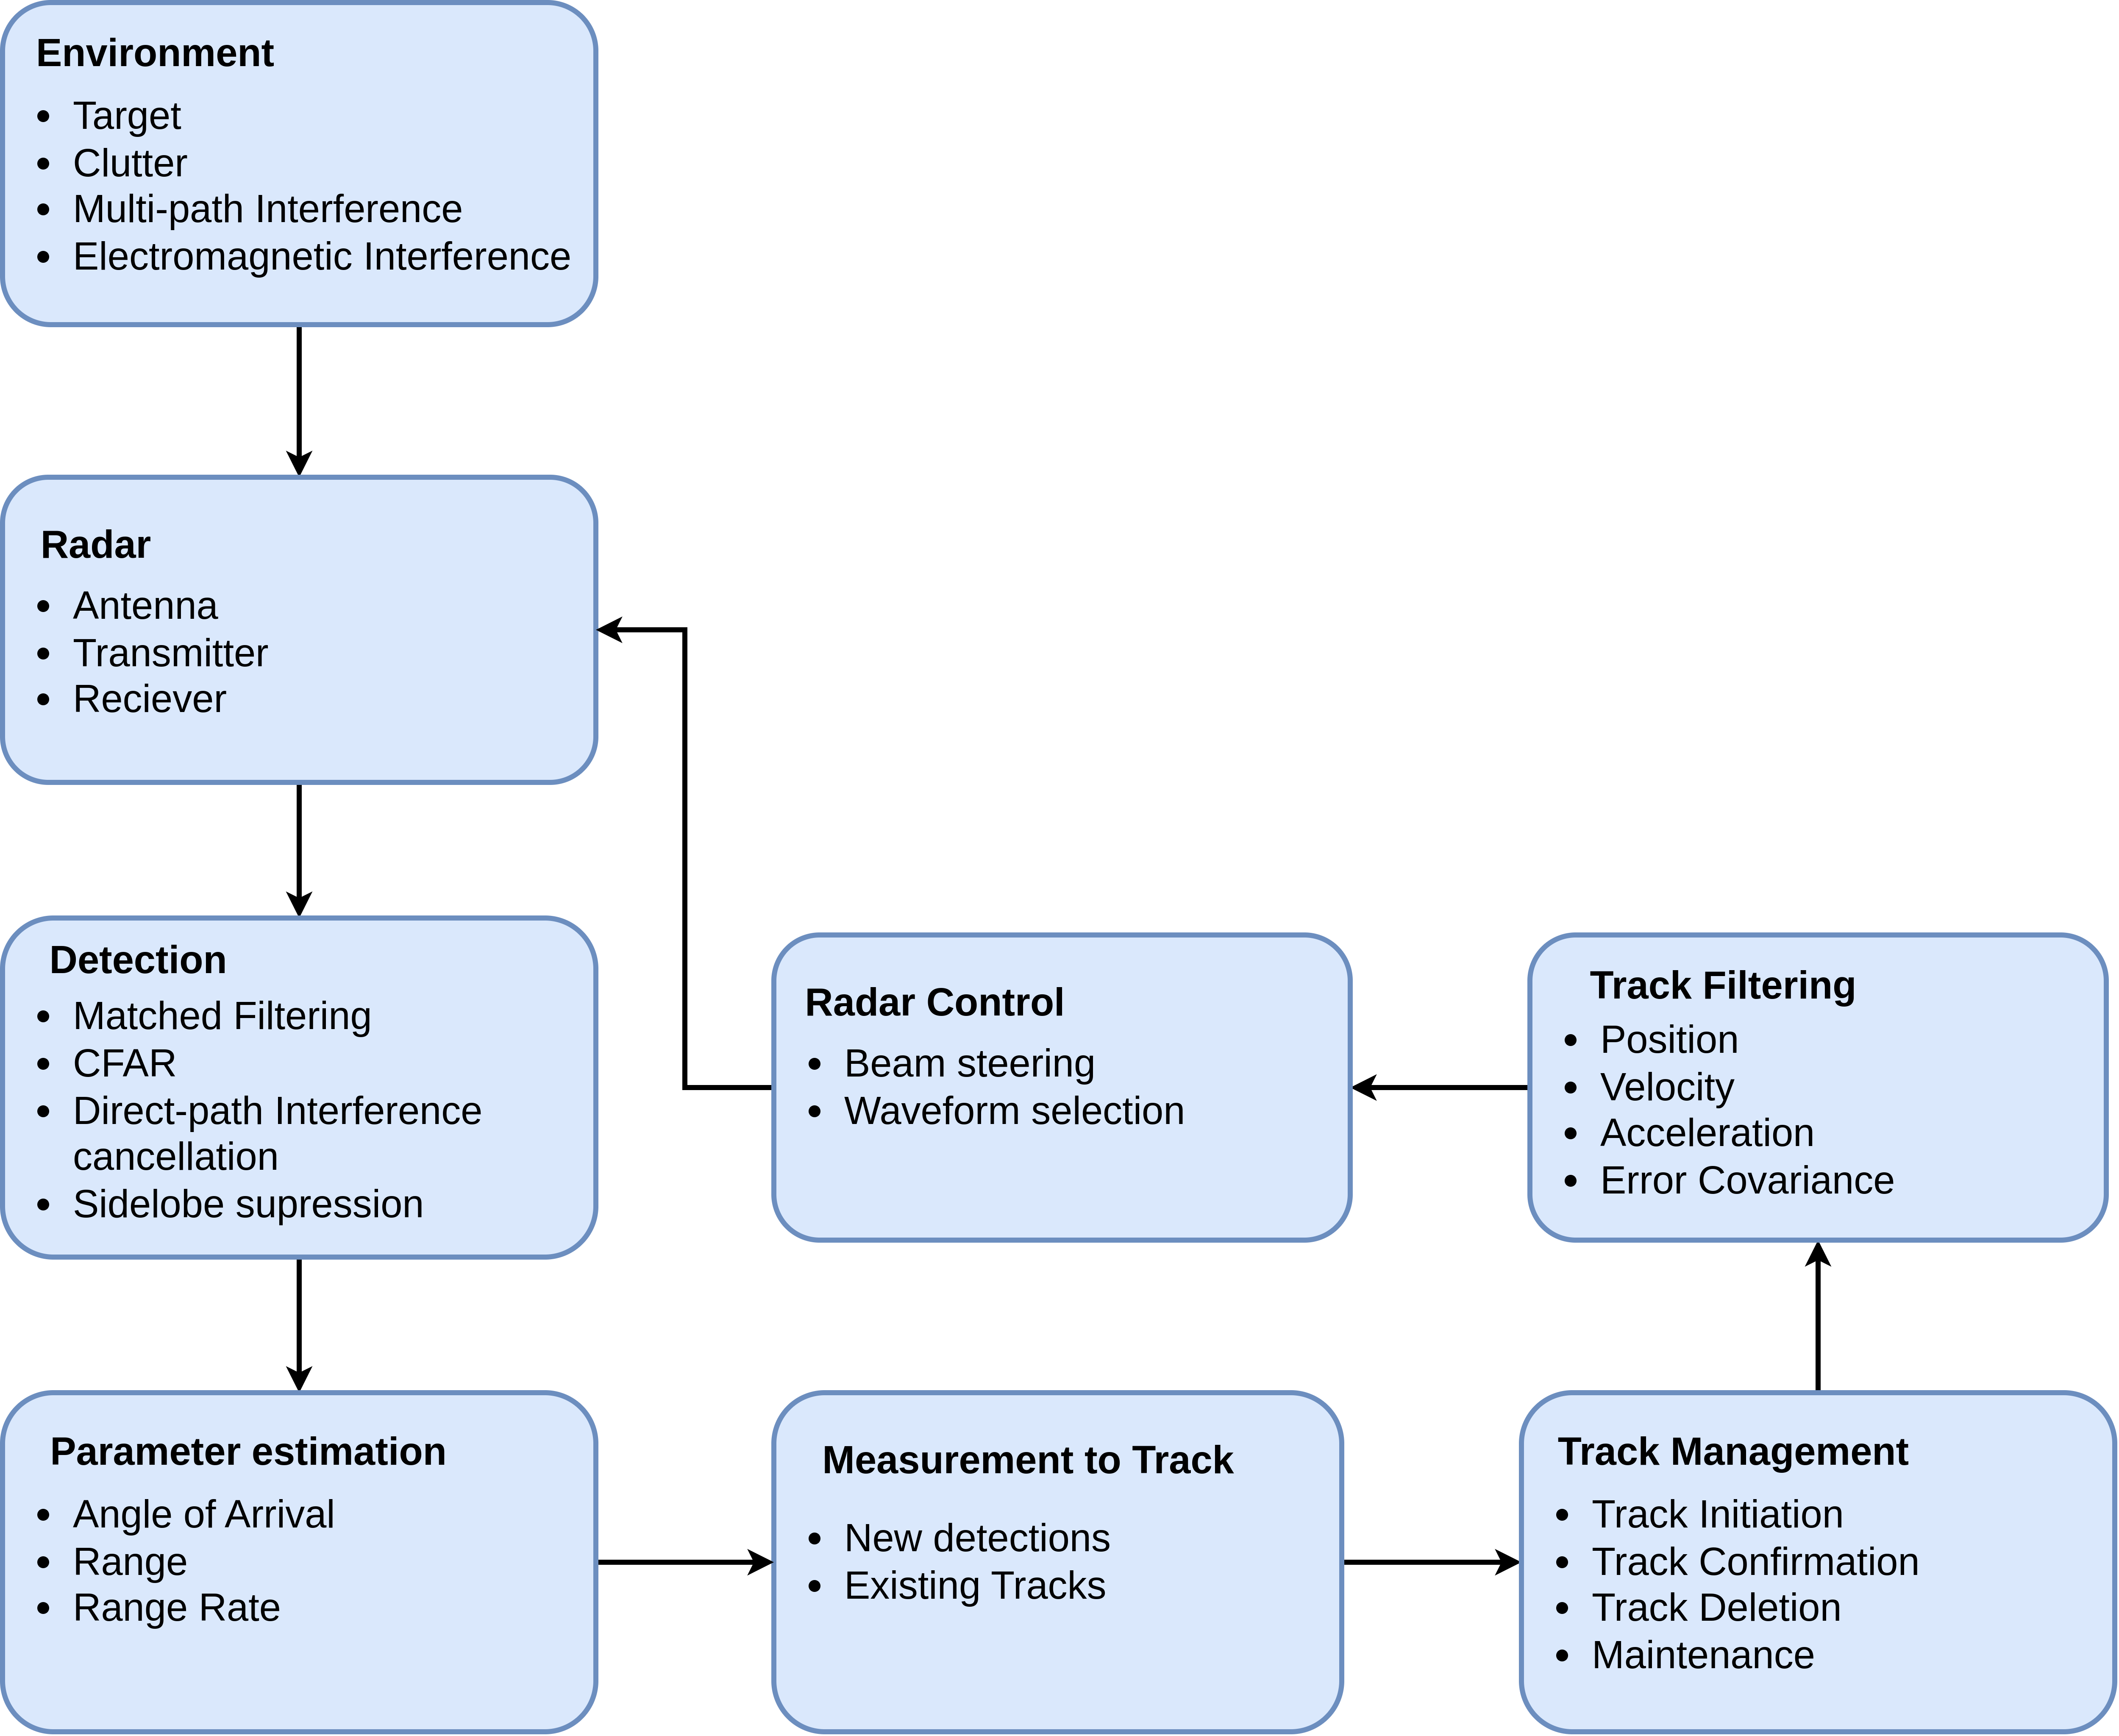
\includegraphics[width=1\linewidth]{Figure/Process.drawio.png}
	\caption{Processing chain for a MTT Radar system.}
	\label{fig1:multi-target}
\end{figure}
%Recursive Bayesian Estimation - TYPES OF Estimators in Estimation Theory%

For stochastic state estimation, the measurements are defined in Equation (\ref{measurement_eq}), the dynamical motion model is given in Equation (\ref{dynamic_model}), and the variables are described in Table \ref{dynamic_model}.
\begin{equation}
    Z_k=H_kX_k+w_k
    \label{measurement_eq}
\end{equation}
\begin{equation}
    X_{k+1} = F_kX_k+G_kv_k
    \label{dynamic_model}
\end{equation}

\begin{table}[ht!]
    \centering
    \large
    \caption{Description of Variables for Stochastic State Estimation.}
    \label{tab:state_estimation_variables}
    \begin{tabular}{lp{12cm}} % Adjust the width (8cm) as needed
        \toprule
        Variable & Description \\
        \midrule
        \( Z_k \)       & Measurement vector at time step \( k \), representing the observed data. \\
        \( H_k \)       & Observation matrix at time step \( k \). \\
        \( X_k \)       & State vector at time step \( k \). \\
        \( w_k \)       & Measurement noise at time step \( k \), typically zero-mean Gaussian noise with covariance \( R_k \). \\
        \( X_{k+1} \)   & Predicted state vector at time step \( k+1 \). \\
        \( F_k \)       & State transition matrix at time step \( k \). \\
        \( G_k \)       & Control input matrix at time step \( k \). \\
        \( v_k \)       & Process noise at time step \( k \), typically zero-mean Gaussian noise with covariance \( Q_k \). \\
        \bottomrule
    \end{tabular}
\end{table}

In a \ac{NCV} motion model, the target's state vector in a scalar coordinate system is described by Equation (\ref{xk}) \cite{Richards2010}. Here $x_k$ represents the target's position at time $t_k$ and $\dot{x_k}$ represents the target's velocity. The process noise is also included to account for uncertainties related to unknown maneuvers and unmodeled dynamics of the target being tracked.
\begin{equation}
    X_k=[x_k\; \dot{x_k}]^T
    \label{xk}
\end{equation}

Malik and Salih\cite{Salih2011} define filtering as the process of ``estimating the state of the system based on measured observations, with the system being represented by its state-space model''. With every new state, the filtering process attempts to estimate the state of the system prior to the measurements. When new measurements become available, the estimation is updated and a new estimation for the next state is calculated \cite{CHEN2}. \textit{Prediction} is a preliminary estimation method that infers the expected value of a quantity at a future time \( t + \tau \) (\( \tau > 0 \)) based on data available up to time \( t \). In the Equations (\ref{1a}) and (\ref{1b}), the generic stochastic filtering problem is considered in a dynamic state-space form.

\begin{equation}
    \dot{x_t} = f(t,x_t,u_t,d_t)
    \label{1a}
\end{equation}
\begin{equation}
        y_t=g(t,x_t,u_t,v_t)
        \label{1b}
\end{equation}

Equations (\ref{1a}) and (\ref{1b}) are known as the state and measurement equations, respectively. Here, \( x_t \) denotes the state vector, \( y_t \) represents the measurement vector, and \( u_t \) is the system input vector in a controlled setting. The terms \( d_t \) and \( v_t \) correspond to process noise and measurement noise, respectively. While the formulation above is in the time domain, discrete-time filtering is typically emphasized in practical applications, as illustrated in Equations (\ref{1c}) and (\ref{1d}).

\begin{equation}
    x_{n+1} = f(x_n,d_n)
    \label{1c}
\end{equation}
\begin{equation}
    y_n=g(x_n,v_n)
    \label{1d}
\end{equation}

In the discrete-time domain, \( d_n \) and \( v_n \) are treated as white noise random sequences with uncertain statistical characteristics. According to Chen \cite{CHEN2}, Equations (\ref{1c}) and (\ref{1d}) simplify to a special case in which a linear Gaussian dynamic system is assumed.
\begin{equation}
    x_{n+1} = F_{n+1},x_n +d_n
    \label{1e}
\end{equation}
\begin{equation}
    y_n=G_nx_n+v_n
    \label{1f}
\end{equation}

The analytic filtering solution is discussed in the Kalman Filtering solution. The Equations (\ref{1e}) and (\ref{1f}) are the transition matrix and measurement matrix respectively.

\section{Kalman Filter Theory}
This section covers the theory and formulation of the Kalman Filter and the \ac{UKF}. It begins with an overview of their frameworks, detailing the mathematical foundations. The algorithms for implementing these filters, namely the prediction and update steps are also discussed in this section. 

\subsection{Kalman Filter}
As noted in the literature, the Kalman Filter algorithm is widely used and useful for estimating the state of a dynamic system based on a sequence of noisy measurements. It is recognized for its efficiency as a recursive, weighted least-squares estimator, assuming that the error statistics follow Gaussian probability distributions \cite{Karlgaard2006}. The Kalman Filter is particularly effective in tracking targets with linear or non-maneuvering trajectories \cite{Bauermeister2016}. The equations governing the Kalman Filter are discussed in the subsequent subsection.

\subsubsection{Principles of Kalman Filtering }
The Kalman Filter is composed of several mathematical equations that define the prediction and the update stage, which operate together as a feedback control mechanism \cite{Adyn}. In the diagram in Figure \ref{fig1:kalmanFilter} from \cite{Adyn}, The Kalman Filter operates by first making a prediction and then applying a correction step to correct and estimate the states of the system. The main idea is that by using information about the state dynamics, the filter forecasts and predicts the subsequent state. As noted in \cite{KalmanTut} a straightforward example is that if I know my previous position (previous state) and my speed (state dynamics), I can estimate my current position (current state).
\begin{figure}[H]
	\centering
	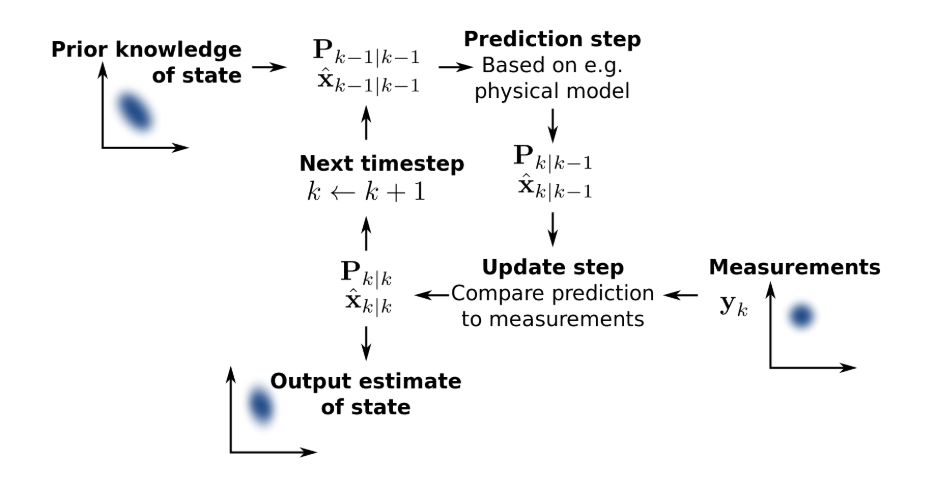
\includegraphics[width=1\linewidth]{Figure/kalmanfilter.PNG}
	\caption{Concept of Kalman Filtering.}
	\label{fig1:kalmanFilter}
\end{figure}

The process model that governs the evolution of the state from time $k-1$ to time $k$ is given by Equation (\ref{kalman_process_model}) :
\begin{equation}
    x_k =Fx_{k-1}+Bu_{k-1} +w_{k-1}
    \label{kalman_process_model}
\end{equation}

Similarly to  \cite{Kim} where $F$ is denoted as the state transition matrix,  whose product with a state vector at an earlier time can give the state at a later time, is applied to the previous state vector $x_{k-1}$. $B$ represents the control-input matrix applied to the control vector $u_{k-1}$, while $w_{k-1}$ is the process noise vector, assumed to follow a zero-mean Gaussian distribution with covariance $Q$.

The process model has a measurement model associated with it, which describes the relationship between the state and the measurement at the current time step k as shown in Equation (\ref{kalman_measure_model}):
\begin{equation}
    z_k=Hx_k+v_k
    \label{kalman_measure_model}
\end{equation}

As described in \cite{Kim}, ``$z_k$ is the measurement vector, H is the measurement matrix, and $v_k$ is the measurement noise vector that is assumed to be zero-mean Gaussian with covariance R i.e.,$v_k \sim  \textit{N}(0,R)$''. Given an initial estimate $x_0$ and a sequence of measurements $\{z_1, z_2, \dots\}$, the system evolution is governed by $F$, $B$, $H$, $Q$, and $R$. The Kalman Filter then uses this information to estimate $x_k$ at time step $k$.


\subsubsection{The Kalman Filter Algorithm}
The Kalman Filter algorithm is composed of two stages: the prediction and update stages. These stages are commonly referred to as the "propagation" and "correction" phases \cite{Kim}.

\paragraph{Kalman Filter Prediction Stage}\mbox{}

The prediction stage involves estimating the state as shown in Equation (\ref{eq:predicted_state}) and error covariance shown in Equation (\ref{eq:predicted_covariance}) at time \( k \) based on the previous state and control input.

\begin{equation}
\hat{x}_k^- = F \hat{x}^+_{k-1} + B u_{k-1}
\label{eq:predicted_state}
\end{equation}
\begin{equation}
P_k^- = F P^+_{k-1} F^T + Q
\label{eq:predicted_covariance}
\end{equation}

\paragraph{Kalman Filter Update Stage}\mbox{}

The update stage refines the predicted estimates using the measurement data, where the Equations in (\ref{eq:measurement_residual})-(\ref{eq:updated_covariance}) are used.

\begin{equation}
\tilde{y}_k = z_k - H \hat{x}^-_k
\label{eq:measurement_residual}
\end{equation}
\begin{equation}
K_k = P^-_k H^T \left( R + H P^-_k H^T \right)^{-1}
\label{eq:kalman_gain}
\end{equation}
\begin{equation}
\hat{x}^+_k = \hat{x}^-_k + K_k \tilde{y}_k
\label{eq:updated_state}
\end{equation}
\begin{equation}
P^+_k = (I - K_k H) P^-_k
\label{eq:updated_covariance}
\end{equation}

In the equations presented in Equations (\ref{eq:predicted_state})-(\ref{eq:updated_covariance}), the hat operator $\hat{}$ is used to denote the estimate of a variable, while the superscripts $-$ and $+$ indicate the predicted and updated estimates respectively. The term $P$ refers to the state error covariance. The covariance of the random variable $x$ is given by $cov(x) = \mathbb{E}[(x-(\hat x)(x-(\hat x)^T]$ where $\mathbb{E}$ represents the expected value operator, which computes the mean of its argument.


During the update process, $\tilde{y}_k$ which represents the measurement residual is first calculated as the difference between the actual measurement $z_k$ and the predicted measurement $H\hat{x}^-_k$. Furthermore, the predicted state is multiplied by the measurement matrix $H$ to estimate the current measurement. To refine the predicted estimate $\hat{x}_k^-$, the residual $y_k$ is scaled by the Kalman gain $K_k$. This results in an updated state estimate. Following this update, the error covariance $P_k^+$ is recomputed.


An effective initialization is crucial for implementing the Kalman Filter successfully. The initial state estimate $\hat{x}^+_0$, the initial error covariance matrix $P^+_0$, and the noise covariance matrices $Q$ and $R$ play a vital role in determining the filter's performance. For instance, selecting a large $P^+_0$ can lead to faster convergence, while incorrect values for the measurement covariance matrix $R$ can adversely affect the integration of measurements. The Kalman Filter algorithm is illustrated in Algorithm \ref{alg:kalman_filter}.\footnote{The Matlab code for the algorithm's implementation can be found in the code repository from Appendix \ref{appendix:repo}.}
\newline
\begin{algorithm}[H]
\caption{Kalman Filter Algorithm for State Estimation.}
\label{alg:kalman_filter}
\begin{algorithmic}[1]
    \vspace{0.6em}
    \State \textbf{Initialize:} $\mathbf{x}_0$, $\mathbf{P}_0$, $\mathbf{Q}$, $\mathbf{R}$
    \vspace{1em}
    
    \State \textbf{Prediction:}
    \vspace{0.6em}
    \State $\mathbf{x}_{k|k-1} \gets \mathbf{A}\mathbf{x}_{k-1|k-1} + \mathbf{B}\mathbf{u}_{k-1}$
    \vspace{0.6em}
    \State $\mathbf{P}_{k|k-1} \gets \mathbf{A}\mathbf{P}_{k-1|k-1}\mathbf{A}^\top + \mathbf{Q}$
    \vspace{1em}
    
    \State \textbf{Update:}
    \vspace{0.6em}
    \State $\mathbf{K}_k \gets \mathbf{P}_{k|k-1}\mathbf{H}^\top(\mathbf{H}\mathbf{P}_{k|k-1}\mathbf{H}^\top + \mathbf{R})^{-1}$
    \vspace{0.6em}
    \If{observation $\mathbf{z}_k$ is available}
        \vspace{0.3em}
        \State $\mathbf{x}_{k|k} \gets \mathbf{x}_{k|k-1} + \mathbf{K}_k(\mathbf{z}_k - \mathbf{H}\mathbf{x}_{k|k-1})$
        \vspace{0.3em}
    \EndIf
    \vspace{0.6em}
    \State $\mathbf{P}_{k|k} \gets (\mathbf{I} - \mathbf{K}_k\mathbf{H})\mathbf{P}_{k|k-1}$
    \vspace{0.6em}
\end{algorithmic}
\end{algorithm}

The Kalman Filter operates under the assumption that both the process and measurement models follow a linear structure, meaning that the relationships between the states, state transitions, and measurements can be expressed using linear equations with the matrices $F$, $B$, and $H$. Additionally, the process and measurement noise are assumed to be additive Gaussian \cite{Kim}. This assumption can be a limitation when the actual observations deviate from the Gaussian assumptions. In the next subsection, a variant of the Kalman Filter designed to handle non-linear models will be discussed.

\subsection{Unscented Kalman Filter}
The implementation of the \ac{UKF} involves the utilization of sampling points known as sigma points. This stands in contrast to the traditional Kalman Filter, where only a singular point (mean) is propagated. In the context of the \ac{UKF}, multiple sigma points are propagated through the linear or non-linear function. This process results in a more accurate recovery of the mean and covariance of the state.
\begin{figure}[H]
	\centering
	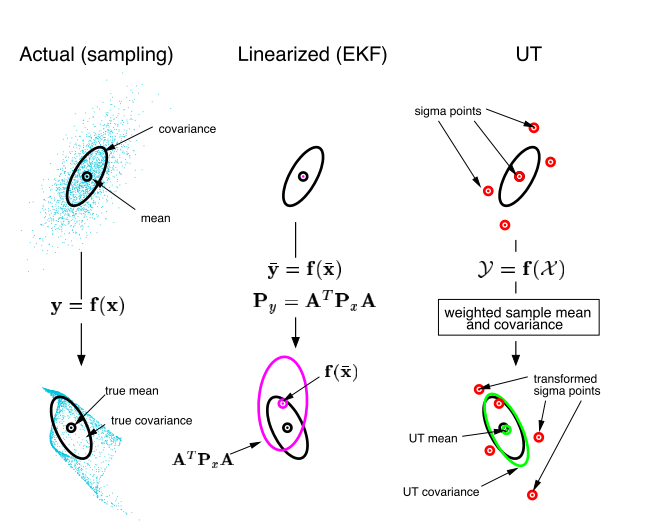
\includegraphics[width=1.1\linewidth]{Figure/UKF.png}
	\caption{Comparison of Monte Carlo methods, EKF, and UKF processes. Left: Monte Carlo sampling representing actual distribution, Middle: Linearized EKF approach, Right: UT applied in the UKF.}
	\label{fig1:UKF}
\end{figure}

\noindent  This approach to filtering diverges from conventional sampling techniques like Monte Carlo methods, including particle filtering, which require a significant number of sample points in order to propagate an accurate distribution of the state \cite{Cai2006}. 
Figure  \ref{fig1:UKF} from \cite{Cai2006} demonstrates how the true mean and covariance evolve in a two-dimensional (2D) system, with Monte Carlo sampling results shown in the left plot; the \ac{EKF} method which uses the linearisation approach is shown in the centre and the right plot shows the \ac{UT} of the \ac{UKF} where only 5 sigma points are necessary for a \ac{2D} system.

In \cite{Julier1997a}, the \ac{UT} is defined as a technique for deriving ``the statistics of a random variable subjected to a non-linear transformation''. It operates on the premise that approximating a Gaussian distribution is simpler than approximating a non-linear function or transformation. By considering the propagation of a random variable \( \mathbf{x} \) with a vector of dimension \( \mathbf{L} \) through a non-linear mapping \( \mathbf{y} = g(\mathbf{x}) \), where \( \mathbf{x} \) has a mean \( \bar{\mathbf{x}} \) and covariance \( \mathbf{P}_x \)  \cite{Cai2006}. The statistics of \( \mathbf{y} \) can be derived using the matrix  \( \mathcal{X} \) of  2\(L\)+1 sigma vectors \( \mathcal{X}_i \) with corresponding weights   \(W_i\) as shown in Equations in (\ref{ukf_equations1}) - (\ref{ukf_equations2}).

\begin{equation}
\begin{aligned}
    \mathcal{X}_0 &= \bar{\mathbf{x}} \\
    \mathcal{X}_i &= \bar{\mathbf{x}} + \left(\sqrt{(L+\lambda)\mathbf{P}_x}\right)_i \quad i = 1,\ldots,L \\
    \mathcal{X}_i &= \bar{\mathbf{x}} + \left(\sqrt{(L+\lambda)\mathbf{P}_x}\right)_{i-L} \quad i = L+1,\ldots,2L
\end{aligned}
\label{ukf_equations1}
\end{equation}

\begin{equation}
\begin{aligned}
    W^{(c)}_0 &= \lambda / (L + \lambda) + (1-\alpha^2 +\beta) \\
    W^{(m)}_0 &= \lambda / (L + \lambda) \\
    W^{(m)}_i &= W^{(c)}_i  = 1/\{2(L + \lambda)\}, \quad i = 1,\ldots,2L\\    
\end{aligned}
\label{ukf_equations2}
\end{equation}

\begin{equation}
\begin{aligned}
    \lambda = \alpha^2(L+\kappa) - L
    \label{lambdaequation}
\end{aligned}
\end{equation}

\(\lambda\) is computed using the Equation in (\ref{lambdaequation}) and all the parameters are described in Table \ref{tab:ukf_parameters}. The \( i \)th row of the square root matrix, denoted as \( \left(\sqrt{(L+\lambda)\mathbf{P}_x}\right)_i \), is used to construct the sigma vectors, which are then passed through the non-linear function shown in Equation (\ref{nonlinear}).


\begin{equation}
    \begin{aligned}
        \mathcal{Y}_i = g(\mathcal{X}_i) \quad i = 0,\ldots,2L
    \end{aligned}
    \label{nonlinear}
\end{equation}

\begin{table}[H]
    \centering
    \large
    \caption{Parameters for Unscented Kalman Filter.}
    \label{tab:ukf_parameters}
    \begin{tabular}{ll}
        \toprule
        Parameter & Description \\
        \midrule
        \( \mathcal{X}_0 \) & Initial sigma point \\
        \( \mathcal{X}_i \) & Sigma points \\
        \( W^{(m)}_i \) & Weight for mean \\
        \( W^{(c)}_i \) & Weight for covariance \\
        \( \lambda \) & Scaling factor \\
        \( \kappa \) & Secondary scaling factor \\
        \( \alpha \) & Distribution of sigma points \\
        \( \beta \) & Incorporation of prior knowledge \\
        \bottomrule
    \end{tabular}
\end{table}
\noindent As stated in \cite{Julier1997a}, ``the mean and covariance for \( \mathbf{y} \) are estimated using a weighted sample mean and covariance of the posterior sigma points,'' as shown in Equations (\ref{equkf1}) and (\ref{equkf2}).  
\begin{equation}
    \begin{aligned}
        \bar{\mathbf{y}} \approx \sum_{i=0}^{2L} W^{(m)}_i \mathcal{Y}_i
    \end{aligned}
    \label{equkf1}
\end{equation}
\begin{equation}
    \begin{aligned}
        \mathbf{P}_x \approx \sum_{i=0}^{2L} W^{(c)}_i \{\mathcal{Y}_i-\bar{\mathbf{y}}\}\{\mathcal{Y}_i-\bar{\mathbf{y}}\}^T
    \end{aligned}
    \label{equkf2}
\end{equation}
\subsubsection{Unscented Kalman Filter Algorithm}
Similar to the Kalman Filter, the \ac{UKF} follows a similar approach to the Kalman filter's state estimation, consisting of the prediction and update stages.

\paragraph{Prediction Stage}\mbox{}

The prediction stage involves creating sigma points, predicting sigma points, computing the predicted state estimate, and calculating the predicted error covariance, as shown in Equations (\ref{eq:create_sigma_points}) to (\ref{eq:predicted_covariance_ukf}) respectively.

\begin{equation}
\mathbf{X}^a_{k-1} = \left[\hat{\mathbf{x}}^a_{k-1} \quad \hat{\mathbf{x}}^a_{k-1} \pm \sqrt{(L+\lambda)\mathbf{P}^a_{k-1}}\right]
\label{eq:create_sigma_points}
\end{equation}
\begin{equation}
\mathbf{X}^x_{k|k-1} = \mathcal{F}\left[\mathbf{X}^x_{k-1}, \mathbf{X}^v_{k-1}\right]
\label{eq:predict_sigma_points}
\end{equation}
\begin{equation}
\hat{\mathbf{x}}^-_k = \sum_{i=0}^{2L} W^{(m)}_i \mathbf{X}^x_{i,k|k-1}
\label{eq:predicted_state_ukf}
\end{equation}
\begin{equation}
\mathbf{P}^-_k = \sum_{i=0}^{2L} W^{(c)}_i \left[\mathbf{X}^x_{i,k|k-1} - \hat{\mathbf{x}}^-_k\right]\left[\mathbf{X}^x_{i,k|k-1} - \hat{\mathbf{x}}^-_k\right]^T
\label{eq:predicted_covariance_ukf}
\end{equation}

\paragraph{Update Stage}\mbox{}

The update stage involves calculating the predicted measurements, the predicted measurement estimate, the innovation covariance, the cross-covariance, the Kalman gain, the updated state estimate, and the revised error covariance, as shown in Equations (\ref{eq:predicted_measurement}) - (\ref{eq:updated_covariance_ukf}) respectively.

\begin{equation}
\mathbf{Y}_{k|k-1} = \mathcal{H}\left[\mathbf{X}^x_{k|k-1}, \mathbf{X}^n_{k-1}\right]
\label{eq:predicted_measurement}
\end{equation}
\begin{equation}
\hat{\mathbf{y}}^-_k = \sum_{i=0}^{2L} W^{(m)}_i \mathbf{Y}_{i,k|k-1}
\label{eq:predicted_measurement_estimate}
\end{equation}
\begin{equation}
\mathbf{P}_{\tilde{y}_k\tilde{y}_k} = \sum_{i=0}^{2L} W^{(c)}_i \left[\mathbf{Y}_{i,k|k-1} - \hat{\mathbf{y}}^-_k\right]\left[\mathbf{Y}_{i,k|k-1} - \hat{\mathbf{y}}^-_k\right]^T
\label{eq:innovation_covariance}
\end{equation}
\begin{equation}
\mathbf{P}_{\mathbf{x}_k\tilde{y}_k} = \sum_{i=0}^{2L} W^{(c)}_i \left[\mathbf{X}^x_{i,k|k-1} - \hat{\mathbf{x}}^-_k\right]\left[\mathbf{Y}_{i,k|k-1} - \hat{\mathbf{y}}^-_k\right]^T
\label{eq:cross_covariance}
\end{equation}
\begin{equation}
\mathcal{K}_k = \mathbf{P}_{\mathbf{x}_k\tilde{y}_k} \mathbf{P}_{\tilde{y}_k\tilde{y}_k}^{-1}
\label{eq:kalman_gain_ukf}
\end{equation}
\begin{equation}
\hat{\mathbf{x}}^+_k = \hat{\mathbf{x}}^-_k + \mathbf{K}_k \left(\mathbf{y}_k - \hat{\mathbf{y}}^-_k\right)
\label{eq:updated_state_ukf}
\end{equation}
\begin{equation}
\mathbf{P}^+_k = \mathbf{P}^-_k - \mathbf{K}_k \mathbf{P}_{\tilde{y}_k\tilde{y}_k} \mathbf{K}_k^T
\label{eq:updated_covariance_ukf}
\end{equation}

The innovation covariance matrix \( \mathbf{P}_{\bar{y}_k\bar{y}_k} \) and the cross-correlation matrix \( \mathbf{P}_{\bar{x}_k\bar{y}_k} \) are computed using the \ac{UT}. Lastly, the Kalman gain \( \mathcal{K} \), the estimated state \( \hat{x}_k \), and the error covariance matrix \( \mathbf{P}_k \) are computed as shown in Equations (\ref{eq:kalman_gain_ukf}) - (\ref{eq:updated_covariance_ukf}). The algorithm for the \ac{UKF} is illustrated in Algorithm \ref{alg:ukf}.\footnote{The Matlab code for the algorithm's implementation can be found in the code repository from Appendix \ref{appendix:repo}.}


\begin{algorithm}[H]
\caption{Unscented Kalman Filter Algorithm}
\label{alg:ukf}
\begin{algorithmic}[1]
    \vspace{0.6em}
    \State \textbf{Initialize:} $\hat{\mathbf{x}}_0$, $\mathbf{P}_0$, $\mathbf{Q}$, $\mathbf{R}$, $\lambda$, $L$, $\alpha$, $\kappa$, $\beta$
    \vspace{0.6em}
    \State Compute weights $W^{(m)}_i$, $W^{(c)}_i$ for $i \gets 0, \dots, 2L$
    \vspace{0.6em}
    \State Sigma points: $\mathbf{X}^a_{0} \gets \left[\hat{\mathbf{x}}_{0} \quad \hat{\mathbf{x}}_{0} \pm \sqrt{(L+\lambda)\mathbf{P}_{0}}\right]$
    \vspace{1em}

    \State \textbf{Prediction:}
    \vspace{0.6em}
    \State $\mathbf{X}^x_{k|k-1} \gets \mathcal{F}\left[\mathbf{X}^a_{k-1}\right]$
    \vspace{0.6em}
    \For{$i \gets 0$ to $2L$}
        \vspace{0.3em}
        \State $\hat{\mathbf{x}}^-_k \gets \hat{\mathbf{x}}^-_k + W^{(m)}_i \mathbf{X}^x_{i,k|k-1}$
        \vspace{0.3em}
    \EndFor
    \vspace{0.6em}
    \For{$i \gets 0$ to $2L$}
        \vspace{0.3em}
        \State $\mathbf{P}^-_k \gets \mathbf{P}^-_k + W^{(c)}_i \left[\mathbf{X}^x_{i,k|k-1} - \hat{\mathbf{x}}^-_k\right]\left[\mathbf{X}^x_{i,k|k-1} - \hat{\mathbf{x}}^-_k\right]^T$
        \vspace{0.3em}
    \EndFor
    \vspace{0.6em}
    \State $\mathbf{P}^-_k \gets \mathbf{P}^-_k + \mathbf{Q}$
    
    \vspace{1em}
    \State \textbf{Update:}
    \vspace{0.6em}
    \State $\mathbf{Y}_{k|k-1} \gets \mathcal{H}\left[\mathbf{X}^x_{k|k-1}\right]$
    \vspace{0.6em}
    \State $\hat{\mathbf{y}}^-_k \gets 0$
    \For{$i \gets 0$ to $2L$}
        \vspace{0.3em}
        \State $\hat{\mathbf{y}}^-_k \gets \hat{\mathbf{y}}^-_k + W^{(m)}_i \mathbf{Y}_{i,k|k-1}$
        \vspace{0.3em}
    \EndFor
    
    \vspace{0.6em}
    \State $\mathbf{P}_{\tilde{y}_k\tilde{y}_k} \gets \mathbf{R}$
    \For{$i \gets 0$ to $2L$}
        \vspace{0.3em}
        \State $\mathbf{P}_{\tilde{y}_k\tilde{y}_k} \gets \mathbf{P}_{\tilde{y}_k\tilde{y}_k} + W^{(c)}_i \left[\mathbf{Y}_{i,k|k-1} - \hat{\mathbf{y}}^-_k\right]\left[\mathbf{Y}_{i,k|k-1} - \hat{\mathbf{y}}^-_k\right]^T$
        \vspace{0.3em}
    \EndFor
    
    \vspace{0.6em}
    \State $\mathbf{P}_{\mathbf{x}_k\tilde{y}_k} \gets 0$
    \For{$i \gets 0$ to $2L$}
        \vspace{0.3em}
        \State $\mathbf{P}_{\mathbf{x}_k\tilde{y}_k} 
 \gets \mathbf{P}_{\mathbf{x}_k\tilde{y}_k} + W^{(c)}_i \left[\mathbf{X}^x_{i,k|k-1} - \hat{\mathbf{x}}^-_k\right]\left[\mathbf{Y}_{i,k|k-1} - \hat{\mathbf{y}}^-_k\right]^T$
        \vspace{0.3em}
    \EndFor
    
    \vspace{0.6em}
    \State $\mathbf{K}_k \gets \mathbf{P}_{\mathbf{x}_k\tilde{y}_k} \mathbf{P}_{\tilde{y}_k\tilde{y}_k}^{-1}$
    \vspace{0.6em}
    \If{observation $\mathbf{y}_k$ is available}
        \vspace{0.3em}
        \State $\hat{\mathbf{x}}^+_k \gets \hat{\mathbf{x}}^-_k + \mathbf{K}_k \left(\mathbf{y}_k - \hat{\mathbf{y}}^-_k\right)$
        \vspace{0.3em}
    \EndIf
    \vspace{0.6em}
    \State $\mathbf{P}^+_k \gets \mathbf{P}^-_k - \mathbf{K}_k \mathbf{P}_{\tilde{y}_k\tilde{y}_k} \mathbf{K}_k^T$
    \vspace{0.6em}
\end{algorithmic}
\end{algorithm}
\newpage
\section{Recursive Gauss-Newton Theory}

The recursive form of the Gauss-Newton filter, the \ac{RGNF}, was implemented in \cite{Inggs1} to minimize the computational memory requirement, which has been identified as a major drawback for the Gauss-Newton filter. This derivation leads to a filter that is similar to the Iterated Extended Kalman Filter. The \ac{RGNF} is derived from the Gauss-Newton algorithm, ``which involves weighted least squares estimation and local linearisation'' according to \cite{Inggs1}. The derivations and resulting equations are primarily intended for non-linear models; however, provisions and adaptations are made to accommodate the linear problem.
\subsection{State Space Model}
Firstly, the state-space model is considered for the non-linear case, where the process state is defined by a non-linear differential Equation as shown in (\ref{316}):
\begin{equation}
    D(X(t)) = F(X(t))
    \label{316}
\end{equation}
where \(F\) is a non-linear vector function describing a dynamic process such as the propagation of the state \(X\), which can include position, velocity, acceleration, or other parameters of a target in space. Assuming that the observation mechanism also depends on a non-linear function of the process state, it can be defined as:
\begin{equation}
    Y(t) = G(X(t)) + v(t)
    \label{317}
\end{equation}
Here \(G\) denotes a non-linear function of \(X\) and \(v(t)\) is a Gaussian random vector \cite{roaldje}. Given the non-linear state model, the aim is to estimate the state of the process. In the case of linear models, this could be easily achieved, but for the non-linear case, the approach followed in \cite{Inggs1} is adopted, beginning with the method of local linearisation.

\subsection{Local Linearisation}
From Newton's method of local linearisation, solving the differential equation produces infinitely multiple trajectories based on initial conditions \cite{Inggs1}. However, a known nominal trajectory represented by the state vector \( \bar{X}(t)\) can be determined, satisfying the same differential equation as \(X(t)\) while remaining close to it \cite{Inggs1}. From those properties, the Equation in (\ref{331}) is arrived at with the perturbation vector \(\delta X(t) \).
\begin{equation}
    X(t) =  \bar{X}(t) + \delta X(t)
    \label{331}
\end{equation}
The perturbation vector is small in relation to \(X(t)\)  or \(\bar{X}(t)\) because it is essentially the error in the state estimation and is made of a vector of time-dependent functions. The perturbation vector adheres to the differential Equation in (\ref{pervec}) \cite{Inggs1}:
\begin{equation}
        D(\delta X(t)) =  A(\bar{X}(t))\delta X(t)
        \label{pervec}
\end{equation}
The sensitivity matrix \(A(\bar{X}(t)) \) is defined as : 
\begin{equation}
        A(\bar{X}(t)) = \frac{\partial F(X(t)}{\partial (X(t))}|_{\bar{X}(t)}
\end{equation}
This implies that \(\delta X(t)\) is a linear differential equation with a time-varying coefficient with the following transition equation:
\begin{equation}
    \delta X(t+\zeta) = \Phi (t_n+\zeta,t_n,\bar{X})\delta X(t)
\end{equation}
The transition matrix \(\Phi (t_n+\zeta,t_n,\bar{X})\) describes the system's evolution from \(t_n\) to \(t_n+\zeta\) and is governed by the following differential equation:

\begin{equation}
    \frac{\partial}{\partial \zeta} \Phi(t_{n+\zeta},t_n,\bar{X}) = A(\bar{X}(t_n+\zeta))\Phi(t_{n+\zeta},t_n,\bar{X})
\end{equation}

From the above equations, it can be observed that the true state process can be estimated by approximating the perturbation vector \(\delta X(t)\) which adheres to a linear differential equation. Next, the linear perturbation vector for the non-linear observation scheme is obtained.

\subsection{Observation perturbation vector}
By considering the noise-free vector \(\bar{Y}_n\) which is \(\bar{Y}_n = G(\bar{X}_n\)) where \(G\) is some non-linear function, when subtracted from the actual observation yields the Equation (\ref{noise_free_vector}): 
\begin{equation}
    \delta Y_n = Y_n-\bar{Y}_n
    \label{noise_free_vector}
\end{equation}
The observation perturbation vector can be shown to be related to the state perturbation vector:
\begin{equation}
    \delta Y_n = H(\bar{X}_n\delta X_n) +v_n
\end{equation}
where \(H(\bar{X}_n)\) represents the Jacobean of G evaluated at \(\bar{X}_n\). This matrix is defined as the observation sensitivity matrix and is defined as:
\begin{equation}
    H(\bar{X}_n) =  \frac{\partial F(X_n)}{\partial (X_n}|_{\bar{X}_n}
\end{equation}

\subsubsection{Sequence of Observations}
Assuming  \(L+1\) observations where the observation perturbation is defined as:
\begin{equation}
    \delta \mathbf{Y}_n = \mathbf{T}_n \delta \mathbf{X}_n + v_n 
    \label{326}
\end{equation}
where \(\mathbf{T}_n\) is the total observation vector defined in Equation (\ref{340}).
\begin{equation}
    \mathbf{T}_n = 
    \begin{bmatrix}
        \mathbf{H}(\bar{X}_n) \\
        \mathbf{H}(\bar{X}_{n-1}) \mathbf{\Phi}(t_{n-1},t_n;\bar{X}) \\
        \vdots \\
        \mathbf{H}(\bar{X}_{n-L}) \mathbf{\Phi}(t_{n-L},t_n,\bar{X})
    \end{bmatrix}
    \label{340}
\end{equation}
Using minimum variance estimation, the state perturbation vector can be obtained as Equation (\ref{328}):
\begin{equation}
    \delta \hat{X}_n = (\mathbf{T}^T_n \mathbf{R}_n^{-1} \mathbf{T}_n)^{-1}\mathbf{T}^T_n \mathbf{R}_n^{-1} \delta \mathbf{Y}_n
    \label{328}
\end{equation}
where the covariance matrix \(S_n\) is defined as \(\mathbf{T}^T_n\mathbf{R}_n^{-1}\) and \(R^{-1}_n\) is defined as  the least squares weight matrix. \(R^{-1}_n\)  and is also known as the inverse of the observation error covariance matrix \(R_n\) \cite{Inggs1}.

\subsection{Recursive Gauss-Newton Formulation}
The total observation vector \( \mathbf{T}_n \) can make the filter computationally expensive due to the significant memory requirements associated with \( \mathbf{T}_n \), as observed in Equation (\ref{340}). This computational burden arises because the size of \( \mathbf{T}_n \) increases with the number of observations used for filtering. To alleviate this issue, a recursive formulation is employed by introducing a forgetting factor \( \lambda \), which is less than or equal to 1, into the least squares weight matrix.

Assuming that observations commence at \(n=0\) and all the initial filter values are available, a weight matrix function using the forgetting factor \( \lambda \le 1 \) is adopted to ensure the filter's adaptiveness. This matrix is defined as follows:

\begin{equation}
    R_n^{-1} = 
    \begin{bmatrix}
        R^{-1} & 0 & \cdots & 0 \\
        0 & \lambda R^{-1} & \cdots & 0 \\
        \vdots & \vdots & \ddots & \vdots \\
        0 & 0 & \cdots & \lambda^n R^{-1}
    \end{bmatrix}
    \label{329}
\end{equation}

Furthermore, to simplify the formulation of the state perturbation vector \(\delta \hat{X}_n\), introducing variables \(P_n\) and \(\Gamma_n\) which are defined as: 
\begin{equation}
    P_n = \mathbf{T}^T_n \mathbf{R}_n^{-1} \mathbf{T}_n
    \label{330}
\end{equation}
\begin{equation}
    \Gamma_n = \mathbf{T}^T_n \mathbf{R}_n^{-1} \delta \mathbf{Y}_n
\end{equation}

The Equation in (\ref{328}) can be rewritten as:
\begin{equation}
    \delta \hat{X}_n = P^{-1}_n \Gamma_n
\end{equation}

where \(P_n\) represents the inverse of the filter covariance matrix \(S_n\), \(P_n = S_n^{-1}\). To achieve the recursive update of the perturbation vector, the recursive updates of \(P_n\) and \(\Gamma_n\) are considered \cite{Inggs1}. Following a similar approach to Nadjiasnger in \cite{Inggs1}, from the equations in (\ref{329}) and (\ref{330}), the recursive equation for \(P_n\) is obtained, which is referred to as the discrete quadratic Lyapunov difference equation:

\begin{equation}
    \mathbf{P}_n = \lambda A(\bar{X}_{n-1})^{-T}\mathbf{P}_{n-1}A(\bar{X}_{n-1})^{-1} + H(\bar{X}_n)^T R^{-1}H(\bar{X}_n)
    \label{333}
\end{equation}

The recursive form of \(\Gamma_n\) is obtained as: 
\begin{equation}
    \mathbf{\Gamma}_n = \lambda A(\bar{X}_{n-1})^{-T}\mathbf{\Gamma}_{n-1} + H(\bar{X}_n)^T R^{-1}\delta Y_n
    \label{334}
\end{equation}

From the Equations (\ref{333}) and (\ref{334}), after some derivations, the Equation (\ref{335}) and (\ref{336}) are arrived at:
\begin{equation}
    \delta \hat{X}_n = K_n[Y_n - G(\bar{X}_n) - M(\bar{X}_n)(\hat{X}_{n|n-1} - \bar{X}_n)]
    \label{335}
\end{equation}
 
\begin{equation}
    P^{-1}_{n|n} = \lambda^{-1}[I - K_n H(\bar{X}_n)]P^{-1}_{n|n-1}
    \label{336}
\end{equation}

where \(K_n\) is the observer gain defined as:
\begin{equation}
    K_n = P^{-1}_{n|n-1} H(\bar{X}_n)^T [R_n + H(\bar{X}_n) P^{-1}_{n|n-1} H(\bar{X}_n)^T]^{-1}
    \label{337}
\end{equation}

From the recursive equations above, the corrected estimate \(\bar{X}_n\) can be obtained iteratively for a number of iterations until \(\bar{X}_n = \hat{X}_{n-1}\). The Equations (\ref{335}), (\ref{336}) and (\ref{337}) are derived for nonlinear state processes and observation schemes. 
\newline
\newline
For the target tracking problem in this project, the non-linear process and observation functions and their linear approximates are replaced by linear equations similar to the work from \cite{Boyer2012}. For the Equation in (\ref{326}), instead of searching for \(\delta X_n\) to minimize the weighted sum of squares for the perturbation vector, \(Y_n = H X_n + v_n\) is looked at, where \(H\) is the linear observation scheme. The equations arrived at are similar to that of the Iterated Extended Kalman Filter with the exception being the forgetting factor \(\lambda\) \cite{De2015}. From these similarities, the equations presented below are arrived at.
\footnote{The full derivation of the Recursive Gauss Newton Filter can be found in \cite{De2015} and \cite{Inggs1}.}
\subsubsection{Prediction Stage}
In the prediction stage, the state vector \(\hat{X}_n\) and \(P_n\) are  predicted forward to \(t_{n+1}\) using the Equations (\ref{338}) and (\ref{339}) respectively where \(Q\) is the process covariance matrix:
\begin{equation}
        \hat{X}_{n+1|n} = \Phi(t_n,t_{n+1})\hat{X}_n
        \label{338}
\end{equation}
\begin{equation}
    P_{(n+1)}|n = \Phi(t_n,t_{n+1})P^{-1}_n \Phi^T(t_n,t_{n+1}) +Q 
    \label{339}
\end{equation}

\subsubsection{Update Stage}
In the update stage, upon receiving new observations, the first step is to perform the recursive cycle to obtain the observer gain \(K_n\).
\begin{equation}
    K_n = P^{-1}_{n|n-1} H(\bar{X}_n)^T [R_n + H(\bar{X}_n) P^{-1}_{n|n-1} H(\bar{X}_n)^T]^{-1}
    \label{337update}
\end{equation}

Where \(P^{-1}_{n|n-1}\) is the predicted filter co-variance matrix, \(R_n\) is the measurement co-variance matrix and \(H\) is the linear observation matrix. Using the computed value of \(K_n\), the updated state estimate \(\hat{X}_{n|n}\) is obtained by:
\begin{equation}
    \hat{X}_{n|n} = \hat{X}_{n|n-1} + K_n[Y_n-H\hat{X}_{n|n-1}]
\end{equation}

Here \(\hat{X}_{n|n-1}\) is the predicted state vector and the iteration stage ends when a set number of iterations is met. Lastly, the filter covariance is updated as shown in Equation (\ref{filter_cov}) : 
\begin{equation}
    P^{-1}_{n|n}= \lambda^{-1}[I-K_nH]P^{-1}_{n|n-1}
    \label{filter_cov}
\end{equation}
The equations derived for the \ac{RGNF} exhibit strong similarities to those of the Kalman Filter. While it might seem convoluted to refer to these equations as the \ac{RGNF}, notable differences such as the forgetting factor and the iterative phase for obtaining the observer gain distinguish them. The \ac{RGNF} discussed here is an evolution of the Gauss-Newton filter by Morrison \cite{Morrison}, later adapted to a recursive version by Nadjiasnger \cite{improvedGauss}. The consolidated steps for the algorithm of the \ac{RGNF} are illustrated in Algorithm \ref{alg:rgnf}.\footnote{The Matlab code for the algorithm's implementation can be found in the code repository from Appendix \ref{appendix:repo}.}

\begin{algorithm}[H]
\caption{Recursive Gauss-Newton Filter Algorithm}
\label{alg:rgnf}
\begin{algorithmic}[1]
    \vspace{2em}
    \State \textbf{Initialize:} $\mathbf{X}_0$, $\mathbf{P}_0$, $\mathbf{Q}$, $\mathbf{R}$, $\lambda$, $\text{max\_iter}$, tolerance
    \vspace{1em}
    
    \State \textbf{Prediction:}
    \vspace{1em}
    \State $\hat{\mathbf{X}}_{n+1|n} \gets \mathbf{F} (\mathbf{X}_n)$
    \vspace{0.5em}
    \State $\mathbf{P}_{n+1|n} \gets \mathbf{A} \mathbf{P}_n \mathbf{A}^T + \mathbf{Q}$
    \vspace{2em}

    \State \textbf{Update:}
    \vspace{1em}
    \State Set $x_{\text{new}} \gets \hat{\mathbf{X}}_{n+1|n}$
    \vspace{1em}
    \If{observation $\mathbf{Y}_n$ is available}
        \vspace{1em}
        \For{$i \gets 1$ to $\text{max\_iter}$}
            \vspace{1em}
            \State $\mathbf{K}_n \gets \mathbf{P}_{n+1|n} \mathbf{H}^T \left[\mathbf{H} \mathbf{P}_{n+1|n} \mathbf{H}^T + \mathbf{R}\right]^{-1}$
            \vspace{1em}
            \State $\Delta \mathbf{X} \gets \mathbf{K}_n \left[\mathbf{Y}_n - \mathbf{H} x_{\text{new}} - \mathbf{H} \left(\hat{\mathbf{X}}_{n+1|n} - x_{\text{new}}\right)\right]$
            \vspace{1em}
            \State $x_{\text{temp}} \gets x_{\text{new}} + \Delta \mathbf{X}$
            \vspace{1em}
            \If{$\|\Delta \mathbf{X}\| < \text{tolerance}$}
                \vspace{1em}
                \State $x_{\text{new}} \gets x_{\text{temp}}$
                \vspace{1em}
                \State \textbf{break}
            \Else
                \vspace{1em}
                \State $x_{\text{new}} \gets x_{\text{temp}}$
                \vspace{1em}
            \EndIf
            \vspace{1em}
        \EndFor
        \vspace{1em}
    \EndIf
    \vspace{1em}
    \State $\mathbf{P}_{n|n} \gets \lambda^{-1} \left[\mathbf{I} - \mathbf{K}_n \mathbf{H}\right] \mathbf{P}_{n+1|n}$
    \vspace{1em}
    \State $\hat{\mathbf{X}}_{n|n} \gets x_{\text{new}}$
    \vspace{2em}
\end{algorithmic}
\end{algorithm}


%%%%%%%%%%%%%%%%%%%%%%%%%%%%%%%%%%%%%%%%%%%%%%%%%%%%%%%%%%%%%%%%%%%%%%%%%%%%%%%%%%%%%%%%%%%%%%%%%%%%%%%%%%%%%%%%%%%%%%%%
\newpage
\section{Particle  Filter Theory} 
Particle Filters, inherently Bayesian, use a set of weighted samples (particles) to recursively estimate the posterior distribution of a state based on noisy measurements \cite{Zhang2009}. Despite their effectiveness, several challenges arise in real-time processing:
\begin{itemize}
    \item \textbf{Particle Degeneracy}:\\
    One particle's weight becomes significantly higher than the others, reducing diversity and accuracy. Resampling techniques are often employed to help redistribute particle weights more evenly.
    \item \textbf{Sample Impoverishment}:\\
    Diversity diminishes over time, reducing distinct sample values. Increasing the number of particles can help at the cost of increased computational demands. Regularization techniques are usually used to maintain particle diversity to balance computational efficiency and filter accuracy.
\end{itemize}
The \ac{PF} implements the formal Bayesian Recursive filter by using sequential Monte Carlo simulations. As new measurements are obtained, the recursive Bayesian filter updates the posterior \ac{PDF}, which is derived through a Bayesian estimation process. \cite{Bauermeister2016}. This section presents the theoretical concepts underlying \ac{PF} theory.

\subsection{Theoretical Concepts}
Two concepts, namely  Monte Carlo theory and Bayesian probability theory, are discussed to provide the theoretical background for \ac{PF}s, similar to the approach followed in \cite{Bauermeister2016}.

\subsubsection{Bayesian Probability Theory}
From the theory and derivations of the other tracking filters discussed in the previous sections, to estimate the state of a dynamic system, two essential models are required. The \textit{process model}, which defines the temporal evolution of the system state, and the \textit{measurement model}, which describes the observation process, incorporating measurement noise.
 In Bayesian estimation theory, the objective is to estimate the dynamic state by constructing its posterior \ac{PDF}, using all available information, including the set of received measurements. The \ac{PDF} embodies all statistical data related to the state, offering a comprehensive solution to the estimation problem \cite{Arulampalam2007}. A filter based on this method includes two stages, similarly to the other tracking filters discussed, namely:
\begin{itemize}
    \item \textbf{Prediction Stage}: The system model is used to propagate the \ac{PDF} forward from one measurement time to the next.
    \item \textbf{Update Stage}: The latest measurement is used to update the predicted \ac{PDF} using Bayes' theorem. Bayes' theorem is used to update the target state when new observations are available.
\end{itemize}

To discuss Bayes' theorem, a non-linear estimation problem is considered where the state sequence of a target is given by:
\begin{equation}
    x_t = f_t(x_{t-1}, v_{t-1})
    \label{343}
\end{equation}
From Equation (\ref{343}), \(x_t\) is the state sequence and \(t \in \mathbb{N}\), \(f_t\) is a non-linear function of the state \(x_{t-1}\), and \(v_t\) is the process noise. In the update stage, the objective is to iteratively update the \ac{PDF} using measurement data:
\begin{equation}
    z_t = h_t(x_t, n_t)
\end{equation}
where \(h_t\) represents a potentially  non-linear function and \(n_t\) is the measurement noise sequence. The objective is to recursively update the degree of belief about the state \(x_t\) at time  \(t\) based on measurements \(z_{1:t}\). To achieve this, the \ac{PDF} \(p(x_t|z_{1:t})\) is constructed where it is assumed that the initially v \(p(x_0|z_0) \equiv p(x_0)\) where the prior \ac{PDF} is available and \(z_0\) representing no measurements. The process of obtaining the \ac{PDF} is completed in the prediction and update stage \cite{Arulampalam2007}.
\newline
\newline
The prior \ac{PDF} of the state at time \(t\) is obtained through the ``Chapman-Kolmogorov equation'' shown in Equation (\ref{Chap}):
\begin{equation}
    p(x_t|z_{1:t-1}) = \int p(x_t|x_{t-1}) p(x_{t-1}|z_{1:t-1}) \, dx_{t-1}
    \label{Chap}
\end{equation}
where the probabilistic model governing the state evolution \cite{Arulampalam2007}, \(p(x_t|x_{t-1})\), is defined by the system Equation (\ref{343}). At the update stage, when the measurement \(z_t\) is available, the prior \ac{PDF} is refined using Bayes' rule:
\begin{equation}
     p(x_t|z_{1:t}) = \frac{p(z_t|x_t) p(x_t|z_{1:t-1})}{\int p(z_t|x_t) p(x_t|z_{1:t-1}) \, dx_t}
    \label{bayes}
\end{equation}
This update depends on the likelihood function \(p(z_t|x_t)\), which is determined by the measurement model and the known statistics of \(n_t\) \cite{Arulampalam2007}. At this stage, The measurement \( z_t \) is used to update the prior density, resulting in the posterior density of the current state. A more detailed analysis of this process is provided in \cite{Arulampalam2007}.
\newline
\newline
In Particle filtering, the estimation problem is addressed by approximating the prediction and update equations of Bayesian probability theory through random sampling and Monte Carlo techniques, as discussed in the next subsection.

\subsubsection{Monte-Carlo Theory}
Monte Carlo techniques, often referred to as Monte Carlo theory, comprise various computational algorithms that rely on repeated stochastic sampling to obtain numerical solutions \cite{Kay}. These methods leverage randomness to address problems that are deterministic in principle. Applying Monte Carlo sampling to estimation problems involves drawing samples from the posterior distribution \cite{Lang2007}.


For dynamic processes, the objective is to approximate the posterior \ac{PDF} using a collection of weighted random samples. State estimates are then derived from these samples and their corresponding weights. To demonstrate this concept, let:

\begin{equation}
    \{x^i_{0:k}, w^i_k\}_{i=1}^{N_s}
\end{equation}
be a random measure characterizing the posterior \ac{PDF} \(p(x_{0:k} | z_{1:k})\), where:
\begin{equation}
    \{x^i_{0:k}, i=1,\dots,N_s\}    
\end{equation}
represents a set of support points with corresponding weights: 
\begin{equation}
    \{w^i_k, i=1,\dots,N_s\}
\end{equation}
and \(x_{0:k} = \{x_j, j=0,\dots,k\}\) is the set of all states up to time \(k\) \cite{Arulampalam2007}. The posterior \ac{PDF} is then approximated by:
\begin{equation}
    p(x_{0:k} | z_{1:k}) \approx \sum_{i=1}^{N_s} w^i_k \delta(x_{0:k} - x^i_{0:k}),
\end{equation}
where the weights are normalized such that \(\sum_{i=1}^{N_s} w^i_k = 1\), and are chosen using an importance sampling method, which will be discussed in the subsequent section. Monte-Carlo methods are useful for determining mean, variance and \ac{PDF} using a histogram \cite{Kay}.

\subsection{Sequential Importance Resampling Filter}

The foundation of particle filtering lies in the Sequential Importance Sampling (SIS) algorithm. As noted by \cite{NJGordon}, it is ``a Monte Carlo technique used to implement a recursive Bayesian filter.'' The \ac{SIS} algorithm uses particles to approximate the posterior \ac{PDF} of the modelled process. Each particle is assigned a weight, which determines its contribution to the overall process estimate \cite{Bauermeister2016}. As each new measurement is sequentially processed, the algorithm recursively updates the weights. However, as noted earlier in this section, the SIS Particle Filter is susceptible to the degeneracy problem. Degeneracy implies that a significant amount of computational resources are spent updating particles whose contributions to the approximation are negligible. An effective measure of degeneracy was introduced in \cite{sequentialLiu} and is defined as:
\begin{equation}
    N_{eff} = \frac{N_s}{1 + \text{Var}(w^{*i}_k)},
\end{equation}
where \(w^{*i}_t\) is the true weight. The estimate \(\hat{N}_{eff}\) of \(N_{eff}\) can be obtained by:
\begin{equation}
    \hat{N}_{eff} = \frac{1}{\sum_{i=1}^{N_s} (w^i_t)^2},
    \label{352}
\end{equation}
where \(w^i_t\) is the normalized weight and a small value of \(N_{eff}\) indicates severe degeneracy \cite{Arulampalam2007}. To mitigate this issue, Particle Filters incorporating resampling methods, such as the Sequential Importance Resampling (SIR) particle filter and other variants, are typically utilised.
\newline
\newline
The implementation of the \ac{SIR} algorithm involves a prediction and update stage, with resampling performed at each iteration to maintain a sufficient number of effective particles.
\begin{itemize}
    \item \textbf{Prediction}: Each particle is propagated through the system model to obtain particles from the prior time step \(k\): \(x_t(i)^* = f(x_{t-1}(i)^*) + w_{t-1}\), where \(w_{t-1} \sim p(w_{t-1})\).
    \item \textbf{Update}: The update step applies Bayes' rule, as shown in Equation (\ref{bayes}). When measurements are received, the likelihood is used to calculate the weights, shaping the sampled particles from the prior \(p(x_t | x_{t-1})\) to represent samples from the posterior \(p(x_t | x_{t-1}, y_t)\). The resampling step transfers the weight information to the samples.
\end{itemize}

To further illustrate the steps involved in the \ac{SIR} algorithm, the schematic adapted from \cite{Imtiaz2006} is shown in Figure \ref{SIR}.

\begin{figure}[H]
	\centering
	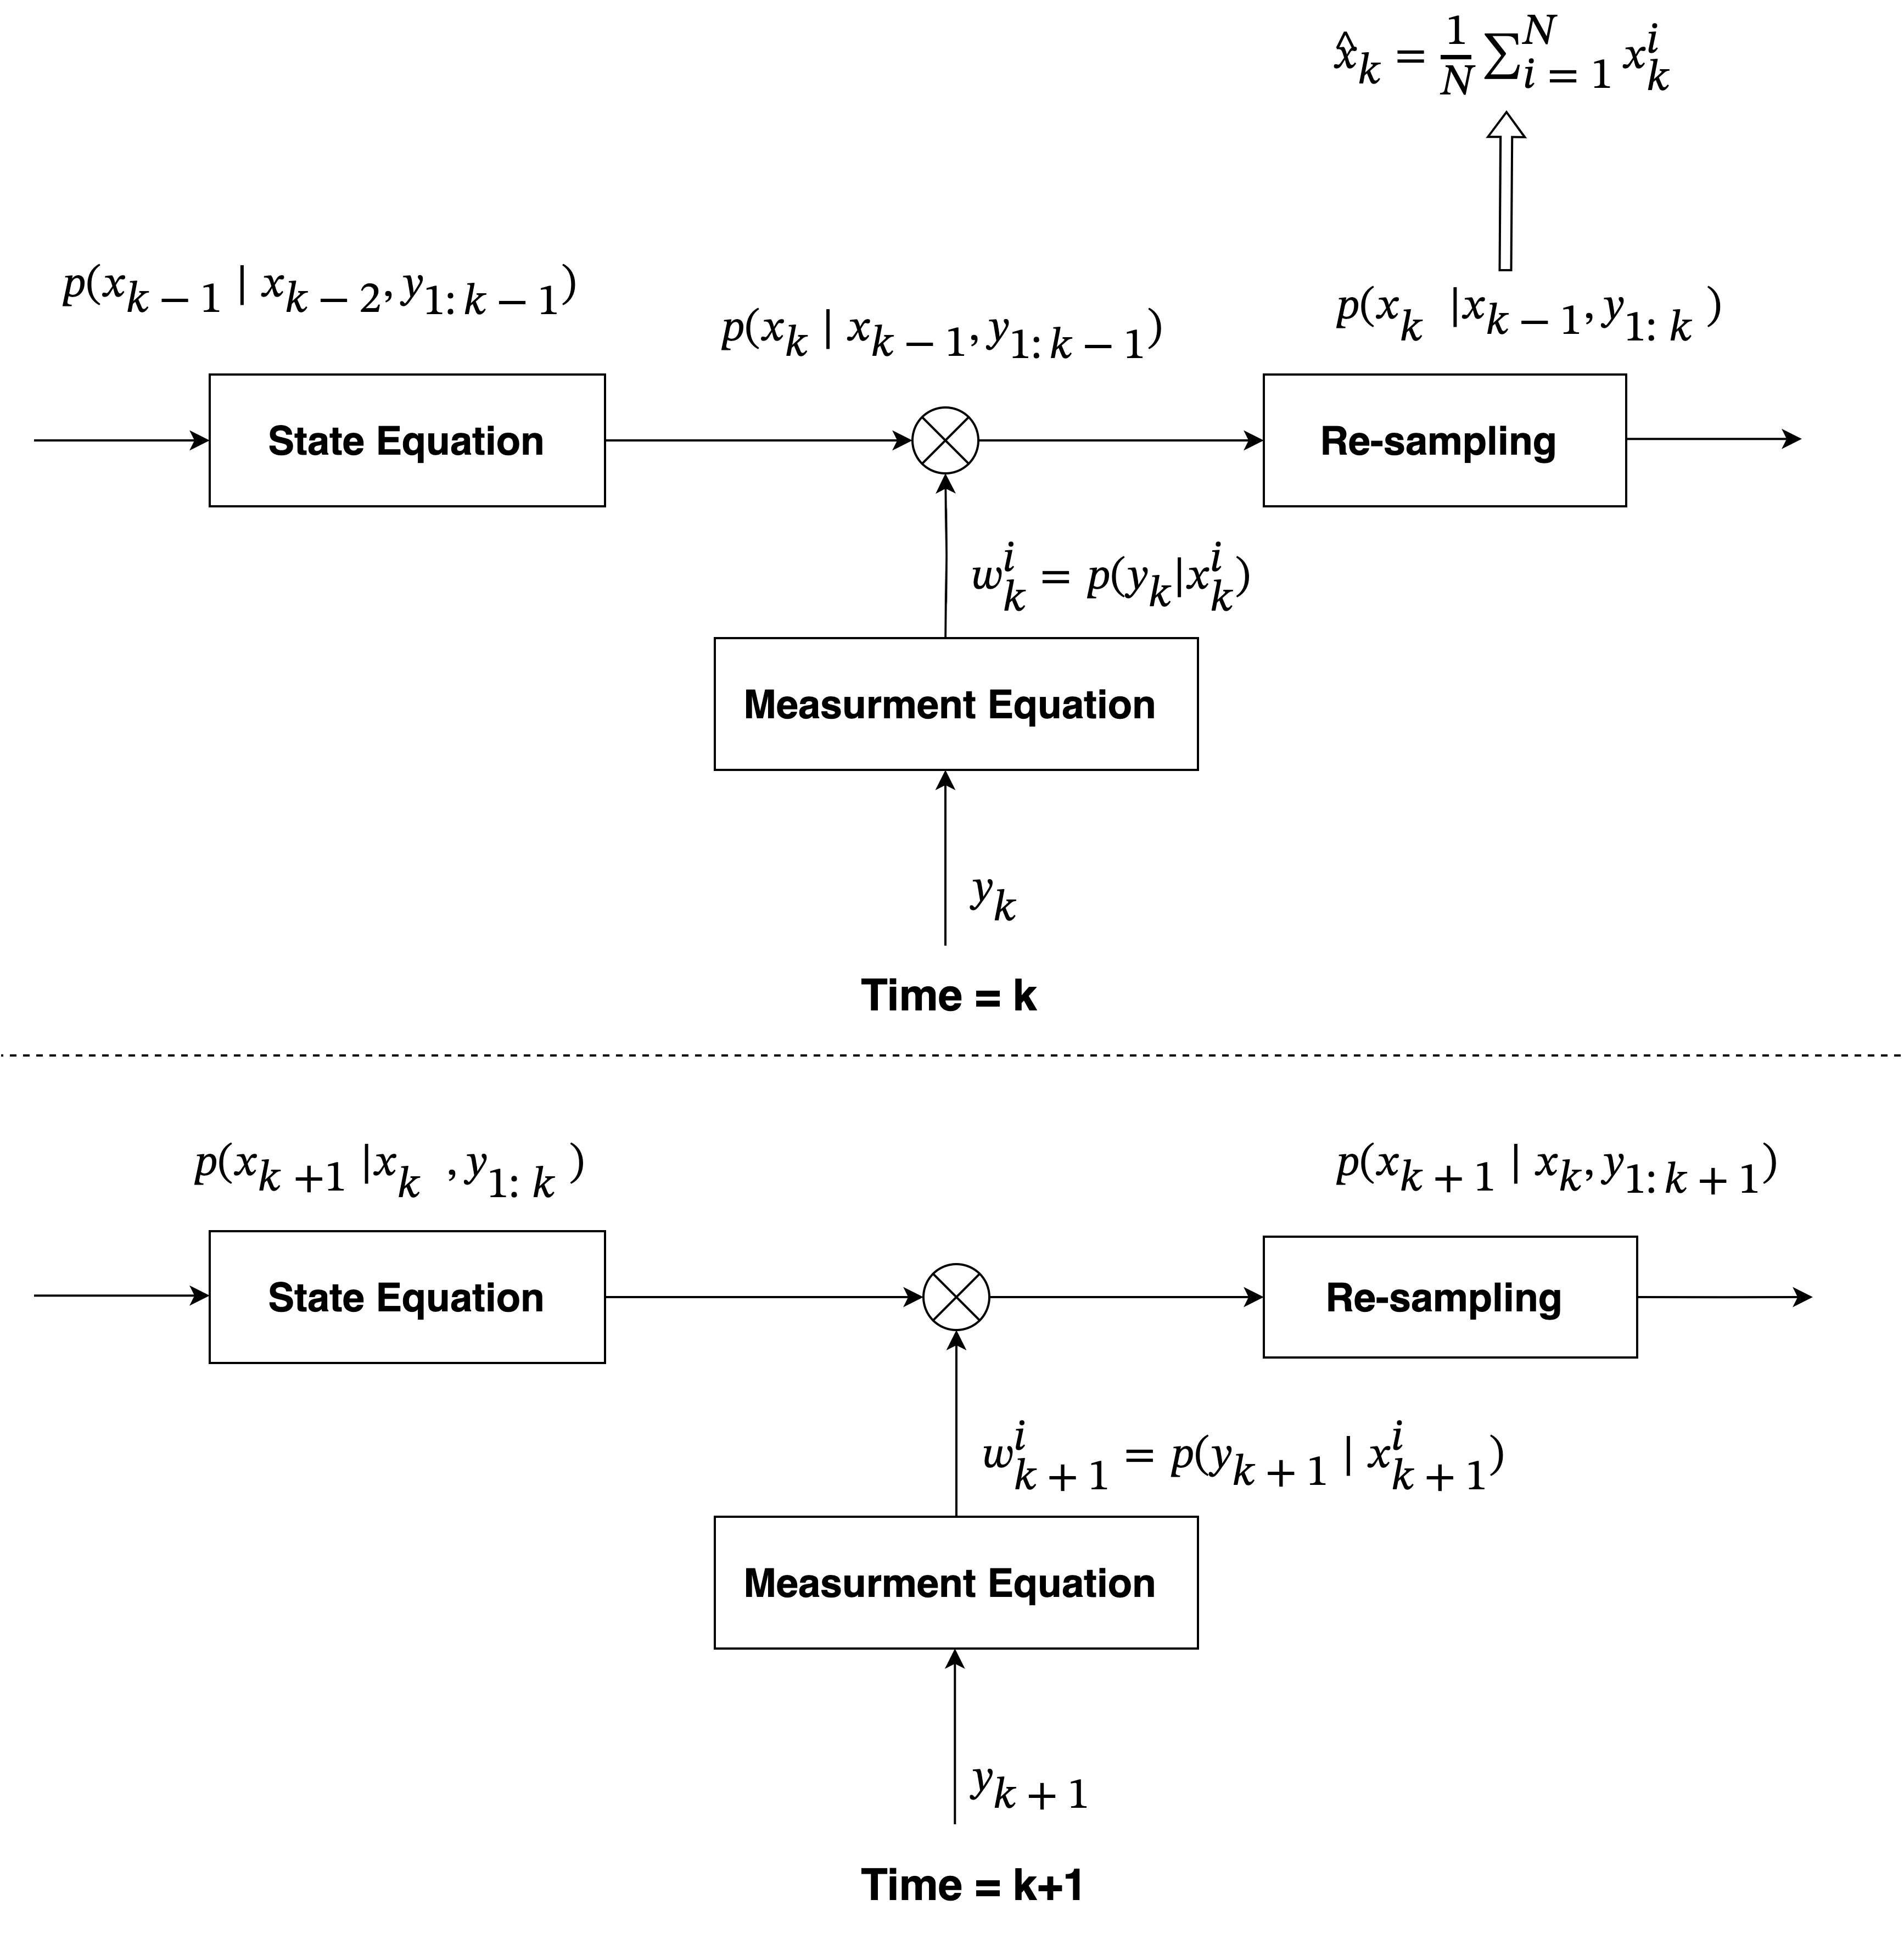
\includegraphics[width=0.75\linewidth]{Figure/SIR1.PNG}
	\caption{Implementation steps of the SIR algorithm.}
        \label{SIR}
\end{figure}

The likelihood calculation for the weights using the measurements is shown in Figure \ref{SIR}. Furthermore, the mean estimate \(\hat{x}_k\) is calculated using the average value. By using  Equation (\ref{352}) to check the number of effective particles, a decision to resample or not can be made at each update, thereby reducing computational load when resampling is unnecessary. In the resampling stage, the less effective particles are replaced by particles with higher weights, ensuring that there is a significant number of particles that accurately represent the state. The algorithm for the \ac{SIR} \ac{PF} is illustrated in Algorithm\ref{alg:particle_filter}.\footnote{The Matlab code for the algorithm's implementation can be found in the code repository from Appendix \ref{appendix:repo}.}


\begin{algorithm}[H]
\caption{Particle Filter Algorithm}
\label{alg:particle_filter}
\begin{algorithmic}[1]
    \vspace{2em}
    \State \textbf{Initialize:}  $\hat{x}_0$,  $\mathbf{Q}$, $\mathbf{R}$, $N$,
    \vspace{0.3em}
    \State $\mathbf{x}_i \sim \mathcal{N}(\hat{x}_0, \mathbf{Q})$, $i \gets 1, \ldots, N$
    \vspace{0.3em}
    \State $w_i \gets \frac{1}{N}$, $i \gets 1, \ldots, N$
    \vspace{1em}
    
    \State \textbf{Prediction:}
    \vspace{1em}
    \For{$i \gets 1$ to $N$}
        \State $\mathbf{x}_i \gets \mathbf{F}(\mathbf{x}_i) + \text{noise}$
        \vspace{0.3em}
        \State $\text{noise} \sim \mathcal{N}(0, \mathbf{Q})$
        \vspace{1em}
    \EndFor
    \vspace{1em}
    
    \State \textbf{Update:}
    \vspace{1em}
    \If{$z_k$ available}
        \vspace{0.5em}
        \For{$i \gets 1$ to $N$}
            \vspace{0.5em}
            \State $p(z_k \mid \mathbf{x}_i) \gets \frac{1}{\sqrt{2 \pi \sigma_{meas}^2}} \exp\left(-\frac{(z_k - h(\mathbf{x}_i))^2}{2 \sigma_{meas}^2}\right)$
            \vspace{0.3em}
            \State $w_i \gets w_i \cdot p(z_k \mid \mathbf{x}_i)$
            \vspace{0.3em}
        \EndFor
        \vspace{0.5em}
        \State $w_i \gets \frac{w_i}{\sum_{j=1}^N w_j}$ for all $i \gets 1, \ldots, N$
    \EndIf
    \vspace{1em}
    
    \State \textbf{Systematic Resampling:}
    \vspace{1em}
    \State $N_{\text{eff}} \gets \frac{1}{\sum_{i=1}^N w_i^2}$
    \vspace{0.5em}
    \If{$N_{\text{eff}} < \frac{N}{2}$}
        \vspace{0.5em}
        \State $\text{cumulative\_weights} \gets \text{cumsum}(w_i)$
        \vspace{0.3em}
        \State $\text{thresholds} \gets \text{linspace}(0, 1 - 1/N, N) + \text{rand}(1, N)/N$
        \vspace{0.3em}
        \For{$i \gets 1$ to $N$}
            \vspace{0.3em}
            \State Find index $j$ such that $\text{thresholds}[i] \le \text{cumulative\_weights}[j]$
            \vspace{0.3em}
            \State $indexes[i] \gets j$
        \EndFor
        \vspace{0.5em}
        \State $\mathbf{x}_i \gets \mathbf{x}_{indexes[i]}$
        \State $w_i \gets \frac{1}{N}$
    \EndIf
    \vspace{1em}
    
    \State \textbf{Estimation:}
    \vspace{1em}
    \For{$i \gets 1$ to $N$}
        \vspace{0.5em}
        \State $\hat{x}_k \gets \hat{x}_k + w_i \mathbf{x}_i$
        \vspace{0.5em}
    \EndFor
    \vspace{1em}
\end{algorithmic}
\end{algorithm}

\section{Adaptive Filtering Theory}
Accurate state estimation is crucial for the performance of tracking filters. The covariance matrices of measurement noise $\mathbf{R}$ and process noise $\mathbf{Q}$ play a significant role in the effectiveness of these filters. To maintain optimal filter performance, these matrices may need to be adjusted dynamically based on the specific use case. Most tracking filters generally perform well when the target behaves according to the assumed process model. However, they can struggle when there are deviations from this model or unexpected events not accounted for by the model. For example, if a filter is designed to track a target moving at a constant velocity with occasional speed changes, it will typically perform well. But if the target suddenly manoeuvres or changes speed in a manner not predicted by the model, the filter's performance may degrade.

Also the presence of outliers in the observations that significantly deviate from the expected distribution can adversely affect filter accuracy. Filters like the Kalman Filter and the \ac{UKF}, which rely on Gaussian assumptions, are particularly sensitive to such deviations. If an observation falls within the tracking gate but deviates significantly from the expected distribution, it can lead to poor estimations. In the context of tracking commercial aircraft, where sudden maneuvers are not anticipated and robust estimations are crucial, it is essential for the filter to handle deviations and outliers effectively. Adjusting the covariance matrices dynamically can help maintain the robustness and accuracy of the filter under varying conditions.
\newline
\newline
According to Mehra \cite{Mehra1972}, approaches to adaptive filtering can be categorized into four types: Bayesian, maximum likelihood (ML), correlation, and covariance matching. In the approach to tracking commercial aircraft for this project, the focus will be on utilizing covariance matching methods for adaptive filtering.

\subsection{Covariance Scaling Theory}
The covariance scaling method focuses on scaling the matrix of the innovation or residual based on their theoretical values. Similarly to the approach introduced in \cite{Akhlaghi2018}, the method for tuning the covariance matrices is discussed. The innovation value and the residual value equations are shown in (\ref{dk}) and (\ref{ek}) respectively which are used for adjusting the covariance matrices.
\begin{equation}
    d_k = \left[ z_k - h_k(\hat{X^-_k})\right]
    \label{dk}
\end{equation}
\begin{equation}
    \varepsilon_k = \left[ z_k - h_k(\hat{X^+_k})\right]
    \label{ek}
\end{equation}
Where \(z_k\) is the measurement and the \(\hat{X}^-_k\) is the predicted state and  \(\hat{X}^+_k\) is the estimated state at time \(k\).Using these values, the measurement covariance matrix \(\mathbf{R}\) and process noise covariance matrix \(\mathbf{Q}\) can be scaled accordingly.

\subsubsection{Adaptive Estimation of \( R \)}

The innovation covariance matrix of the tracking filter at time \( k \) is defined as:

\begin{equation}
    S_k = H_k P^-_k H^T_k + R_k
\end{equation}

where \( H_k \) is the measurement mapping matrix and \( P^-_k \) is the predicted error covariance matrix at time \( k \). The measurement covariance matrix \( R_k \) can be rewritten as:

\begin{equation}
    R_k = S_k - H_k P_k H^T_k
\end{equation}

Theoretically, \( R_k \) should be a positive definite matrix to ensure that the measurement covariance matrix represents a valid probability distribution with non-negative variances. Using the approach from \cite{wang1999stochastic}, \( R_k \) can be estimated by:

\begin{equation}
    \bar{S_k} = \mathbb{E}\left[ \varepsilon_k \varepsilon_k^T \right] 
    \label{357}
\end{equation}

\begin{equation}
    R_k = \mathbb{E}\left[ \varepsilon_k \varepsilon_k^T \right] + H_k P^-_k H_k^T 
    \label{358}
\end{equation}

To implement what is shown in Equation (\ref{358}), the expectation operation of \(\varepsilon_k \varepsilon_k^T\) is approximated by averaging \(\varepsilon_k \varepsilon_k^T\) over time. A moving window with previous residuals is used, or a forgetting factor, similar to the one introduced in \cite{Akhlaghi2018}, can be applied where \(0 \le \alpha \le 1\). A larger value of \(\alpha\) can be used to adaptively estimate \(R_k\) to incur fewer fluctuations and longer time delays when dealing with abrupt changes. The following equation applies:

\begin{equation}
    R_k = \alpha R_{k-1} + (1-\alpha)(\varepsilon_k \varepsilon_k^T + H_k P^-_k H_k^T)
    \label{time_delays}
\end{equation}

At every update, instead of using the normal measurement covariance matrix, the one derived in Equation (\ref{time_delays}) is used for adaptive estimation. Alternatively, the process noise covariance matrix \(Q\) can be adapted when dealing with abrupt changes or outliers in the observations.

\subsubsection{Adaptive Estimation of \( Q \)}

To scale the process noise covariance \( Q \), an approach similar to that proposed in \cite{Ding2007} can be used. For an optimal filter, the predicted innovation covariance matrix should match the one computed from the innovation sequence, as demonstrated in Equation (\ref{357}). Directly resolving \( P^-_k \) from equation(\ref{358}) is not straightforward. Therefore, a simpler method based on the scaling factor introduced in \cite{Ding2007} is used.

The scaling factor \( \alpha \) is defined as:

\begin{equation}
    \alpha = \frac{\text{trace}\{H_k \tilde{P}^-_k H_k^T\}}{\text{trace}\{H_k \hat{P}^-_k H_k^T\}} = \frac{\text{trace}\{\varepsilon_k \varepsilon_k^T - R_k\}}{\text{trace}\{H_k \hat{P}^-_k H_k^T\}}
\end{equation}

Here, \( \alpha \) adjusts the process noise covariance \( Q \) by comparing the traces of the predicted and actual innovation covariance matrices. To derive \( \alpha \), substitute the expression for \( \hat{P}^-_k \):

\begin{equation}
    \hat{P}^-_k = \Phi_{k-1} \hat{P}_{k-1} \Phi_{k-1}^T + Q_{k-1}
\end{equation}

Substituting this into the scaling factor equation gives:

\begin{equation}
    \alpha = \frac{\text{trace}\left\{H_k \left(\Phi_{k-1} \hat{P}_{k-1} \Phi_{k-1}^T + \tilde{Q}_{k-1}\right) H_k^T\right\}}{\text{trace}\left\{H_k \left(\Phi_{k-1} \hat{P}_{k-1} \Phi_{k-1}^T + Q_{k-1}\right) H_k^T\right\}}
\end{equation}

The adaptation rule for \( Q \) is then defined as:

\begin{equation}
    \hat{Q}_k = Q_{k-1} \sqrt{\alpha}
\end{equation}

here the square root in the adaptation rule introduces a smoothing effect, helping to stabilize the adjustment of \( Q \).


\section{Log-Likelihood Statistical Benchmark}

The likelihood function, in probabilistic terms, expresses how probable the observed data is given a set of model parameters. For a given observation \( z_k \) and state prediction \( Hx_k \), the likelihood \( L \) represents the probability of observing \( z_k \), assuming the predicted state \( Hx_k \) and the associated uncertainties in the system. Mathematically, this can be expressed as:

\begin{equation}
    L(z_k | Hx_k) = p(z_k | Hx_k, P, R)
\end{equation}

where \( P \) is the state covariance matrix and \( R \) is the measurement noise covariance matrix. 

The log-likelihood, which is the natural logarithm of the likelihood function as discussed in the literature review, simplifies this expression and is widely used due to its mathematical convenience in optimization and statistical inference \cite{Grewal2006}. For instance, the likelihood for the Kalman Filter residual \( e_k = z_k - Hx_k \), given the system uncertainty \( S = HPH^\top + R \), is expressed as:

\begin{equation}
    L = \frac{1}{\sqrt{2\pi S}} \exp\left( -\frac{1}{2} e_k^\top S^{-1} e_k \right)
    \label{eqLikelihood}
\end{equation}

Taking the natural logarithm of the likelihood, Equation (\ref{eqLogLikelihood}) can be obtained.

\begin{equation}
    \log(L) = -\frac{1}{2} \left( \log(2\pi S) + e_k^\top S^{-1} e_k \right)
    \label{eqLogLikelihood}
\end{equation}

This function evaluates how well the predicted observations align with the actual observations while accounting for uncertainties in both the system and measurements. The log-likelihood offers several advantages, with the main advantage being that the logarithm is a strictly increasing function, meaning it reaches its maximum at the same point as the original likelihood function \cite{labbe2014kalman}.
\newline
\newline
The log-likelihood is related to performance measures such as the \ac{NIS} and the \ac{NEES}, which are widely used to evaluate the accuracy and consistency of tracking filters, as noted in the literature review section.
\newline
The \textit{NEES} is given by:
\begin{equation}
    \epsilon_{x,k} = e_{x,k}^\top P^{-1}_{k|k} e_{x,k}
\end{equation}

where \( e_{x,k} \) is the estimation error between the true state and the predicted state, and \( P_{k|k} \) is the covariance matrix of the estimated state. The \ac{NEES} metric evaluates the accuracy of state estimates by comparing them to the true state of the system. Since calculating \ac{NEES} depends on knowing the true state \( x_k \), it is generally applied in simulation environments or in cases where an external validation system is available \cite{chen2024kalman}.
\newline
The \textit{NIS}, on the other hand, is computed as:
\begin{equation}
    \epsilon_{z,k} = e_k^\top S^{-1}_{k|k-1} e_k
\end{equation}
where \( e_k = z_k - Hx_k \) is the innovation vector, and \( S_{k|k-1} \) is the innovation covariance matrix. Unlike \ac{NEES}, \ac{NIS} does not require ground truth information; it only depends on the observation sequence, making it more suitable for real-world data without access to the true state \cite{chen2018weak}. The performance evaluation performed on the tracking filters in the next chapters focuses on the Log-likelihood function to evaluate the tracking filters due to its ability to provide a direct measure of model fit based on probability theory




\section{Conclusions}
In this chapter, a theoretical study of various tracking filters, adaptive filtering methods, and tracking filter performance was presented, with a focus on their mathematical foundations. The discussion began with an introduction to state-estimation theory, followed by the theory of the tracking filters, including the Kalman Filter, the \ac{UKF}, the \ac{SIR} Particle Filter, and the \ac{RGNF}. This section elucidated their underlying principles, mathematical formulations, and algorithms for use in state estimation of dynamic systems. Additionally, an overview of adaptive filtering methods, particularly those involving covariance scaling were presented. Lastly, the log-likelihood was introduced as a statistical benchmark for performance evaluation.

The next chapter will focus on simulations, implementing the discussed tracking filters, and validating them through simulated aircraft trajectories in the bistatic range and Doppler domains. The performance of the tracking filters will be evaluated using various metrics, including the log-likelihood, to compare their effectiveness in various scenarios.


%----------------------------------------------------------------------------------------
%	Section 4
%----------------------------------------------------------------------------------------
\newpage
\chapter{Simulations}
\section{Introduction}

In the previous chapter, the theoretical framework for the various tracking filters and the adaptive techniques used for tracking our target of interest in the bistatic range and Doppler domain were explored. The primary objective of this dissertation is to implement these tracking filters and rigorously evaluate their performance through simulations. The simulations presented in this chapter are conducted using MATLAB code and \ac{FERS}.
\newline 
\newline
In section 4.1, the \ac{Radar} system overview is outlined. The setup of the simulation environment using \ac{FERS} is discussed in section 4.2, followed by a detailed discussion of the results from the \ac{Radar} processing chain simulations in section 4.3. The formulation of target dynamics is covered in section 4.4. Lastly, the implementation of the tracking filters and the \ac{MTT} are discussed in section 4.5. The evaluation metrics for assessing the performance of the tracking filters is addressed in the next chapter.

\subsection{Radar System Overview}

\ac{Radar} systems can be configured with various architectures, each optimized for specific objectives. In the simulations conducted within this section, the focus is on modelling the targets of interest within a \ac{Radar} environment. Following this, the \ac{Radar} processing chain and the \ac{MTT} system implementation is considered. The flow diagram in Figure \ref{fig:simulationRadar} depicts the key components involved in the overall \ac{Radar} simulation, including the \ac{MTT} system. From the \ac{Radar} System Overview, certain components, such as \ac{DPI} and clutter cancellation, fall outside of the primary scope of this research. However, validating the functionality of these components is crucial to ensure successful target tracking.
\newline
\begin{figure}[H]
    \centering
    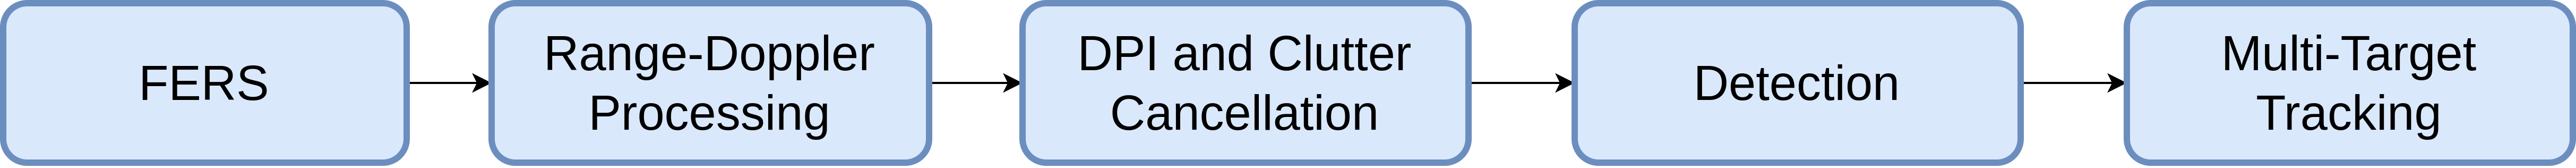
\includegraphics[width=0.95\linewidth]{Figure/radarOverview.drawio.png}
    \vspace{0.5em} 
    \caption{Flow diagram for  Radar System Overview for Simulations.}
    \label{fig:simulationRadar}
\end{figure}

 The simulations will focus on the implementation of some of the components. These components are detailed as follows:

\begin{itemize}

\item \textbf{\ac{FERS}\\} Simulates the behaviour of the \ac{Radar} system, defining various components within the \ac{Radar} environment. The discussion and usage of \ac{FERS} are covered in section 4.2.

\item \textbf{Range and Doppler Processing:}\\
This involves processing the  \ac{Radar} signals from \ac{FERS} into the bistatic range and Doppler domain.

\item \textbf{DPI and Clutter Cancellation:}\\
This component addresses the removal of \ac{DPI} and clutter from the bistatic range and Doppler map. Validation is performed to ensure the algorithm operates correctly.

\item \textbf{Detection:}\\
Detection of targets is achieved using a \ac{CA-CFAR} detection filter, followed by a clustering algorithm to determine target centroids.

\item \textbf{Multi-Target Tracking:}\\
This involves tracking multiple targets based on observations, which includes data association, track management and target state estimation using tracking filters.

\end{itemize}

\section{Flexible Extensible Radar Simulator}

\ac{FERS} was developed from a Ph.D. thesis presented in \cite{fersMarc}, which was based on creating a simulator that supports various \ac{Radar} system configurations. The simulator was introduced as an open-source project to address certain limitations of custom \ac{Radar} simulators, offering the capability to handle an arbitrary number of transmitter/receiver nodes and targets distributed across space and time \cite{inggs2009extensible}. Full documentation of the \ac{FERS} simulator can be found on the project's \href{https://github.com/stpaine/FERS/wiki}{GitHub Wiki page}.
\newline
\begin{figure}[H]
    \centering
    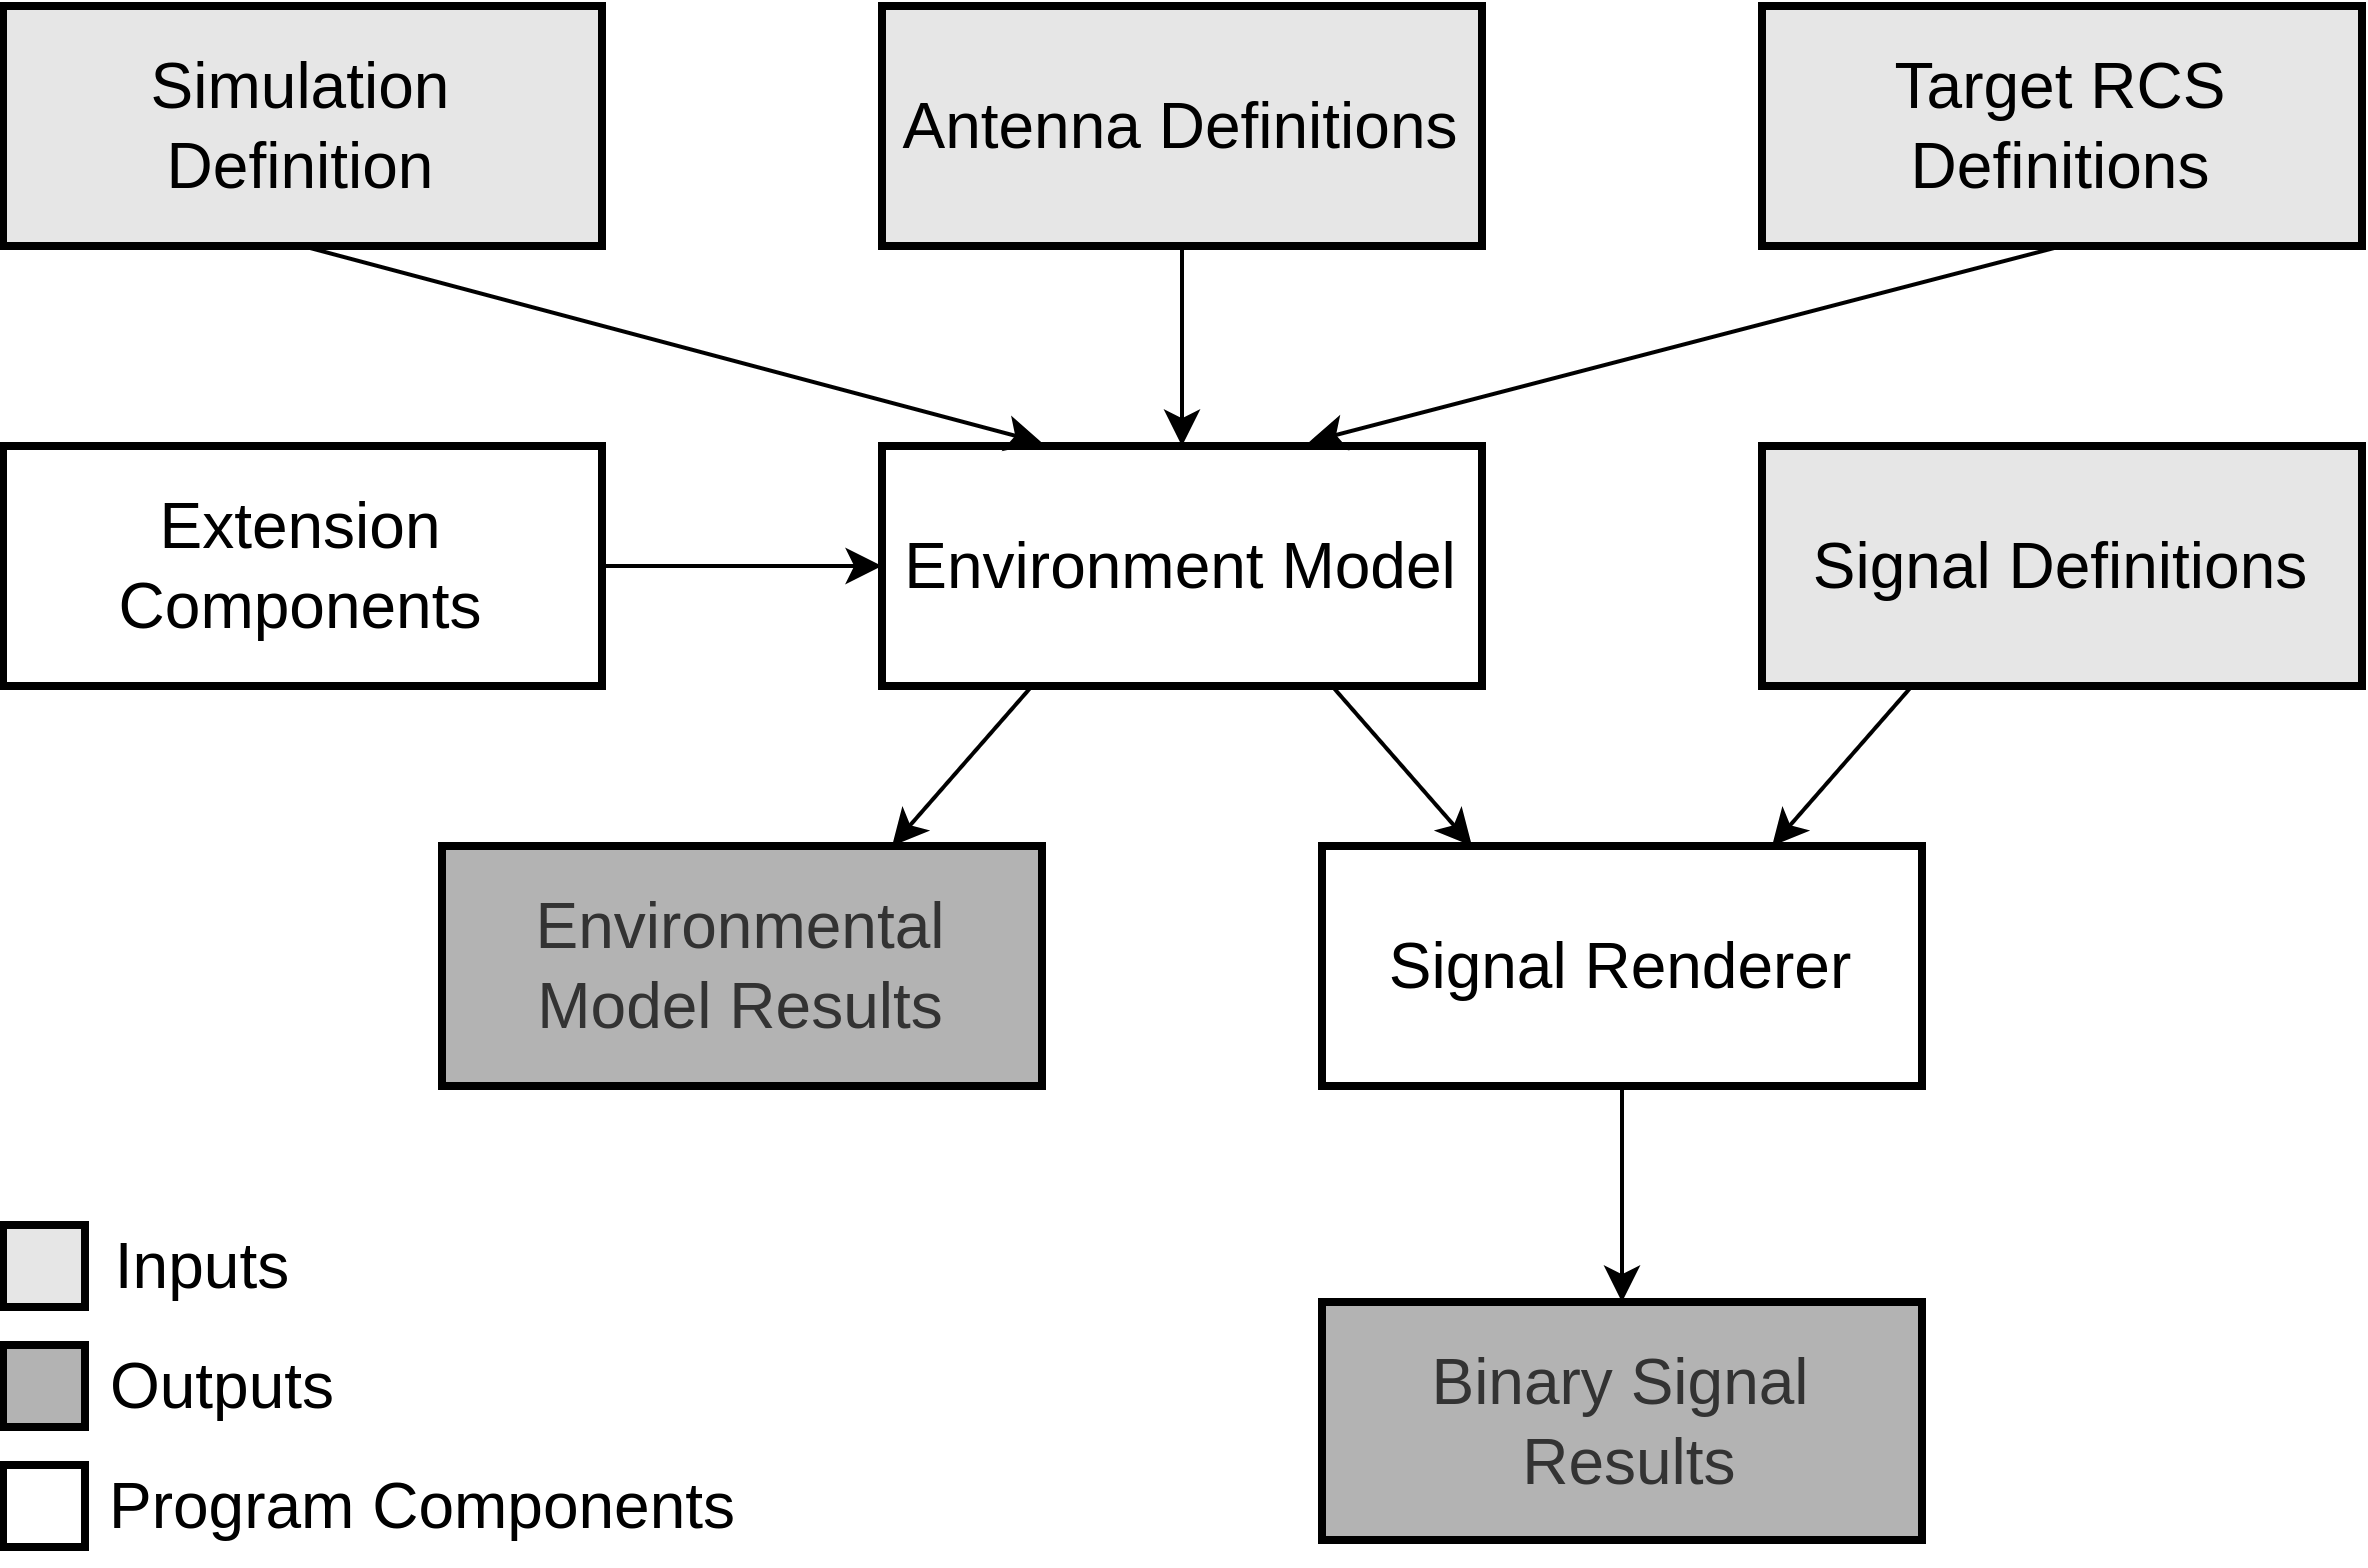
\includegraphics[width=0.75\linewidth]{Figure/fersDataflow.drawio (2).png}
    \vspace{2em}
    \caption{The FERS data flow diagram illustrates the various components  within the FERS Simulator.}
        \label{fig:fers-flow}
\end{figure}

\subsection{FERS Simulation Setup and Configuration}
\ac{FERS} simulator requires several key inputs to define the simulation environment as illustrated in Figure \ref{fig:fers-flow} from \cite{inggs2009extensible}. These inputs include the \ac{Radar} system configuration, environmental parameters, antenna characteristics, the transmitted waveform, and the target's \ac{RCS}. The simulator uses an \ac{XML} file as the input format.

The specific parameters used in \ac{FERS} to achieve the simulation objectives are discussed here. Firstly, the input definitions are discussed, followed by an explanation of the output data that constitutes our simulation results. The internal workings of the simulator are beyond the scope of this project; instead, the focus is on how the input parameters are utilized to produce results that will be validated against the theoretical expectations further in the simulations.


\subsection{Simulation Definition}
The simulation definition in \ac{FERS} consists of several details..

\subsubsection{FERS Simulation Parameters}

The main parameters used in \ac{FERS} for the bistatic \ac{Radar} setup are described in Table \ref{Sim_par_FERS}, the other configurations are outlined in the \ac{XML} code for the different scenarios.

\begin{table}[h]
\centering
\caption{Simulation Parameters.}
\label{Sim_par_FERS}
\begin{tabular}{ll}
\hline
\textbf{Parameter} & \textbf{Value} \\
\hline
Start Time & 0 \\
End Time & Duration of Simulation (s) \\
Sampling Rate & 200 kHz \\
\ac{ADC} Bits & 16 \\
Propagation Speed & Speed of Light (\textit{c}) \\
\hline
\end{tabular}
\end{table}

\subsubsection{Pulse}
Describes the transmitted waveform parameters, including power and carrier frequency. An \ac{FM} waveform signal recorded in Malmesbury is used as the transmitted waveform. The carrier frequency and power are also varied depending on the scenario being simulated.

\subsubsection{Timing}
Specifies the timing source parameters; the frequency of the clock is set to 200 kHz.

\subsubsection{Platform}
Details the platform, its position and its components, such as a receiver, transmitter or target. Three platforms for the transmitter, surveillance and direct receiver channels, along with additional platforms for the targets that are used.

\subsection{Antenna and Target Definition}
The Antenna parameter in the XML defines the antenna gain and pattern. The receiver antennas are set to use directional antennas with a 'sinc' function pattern. The target \ac{RCS} and trajectories are configured depending on the scenario being simulated.

\subsection{Binary Signal Results}
The output data from \ac{FERS} is stored as 64-bit floating point samples in an HDF5 binary file. This file contains the received signals from the receiver terminals as baseband signals (quadrature and in-phase components). These signals are used for processing in the subsequent section to resolve the range and Doppler map.


\section{Processing Chain Implementation}
The components of the processing chain are all implemented in MATLAB code. In the first subsection, the results from the range and Doppler processing using the results from \ac{FERS} are discussed.

\subsection{Range and Doppler Processing}
The problem of target localization using cross-correlation is discussed in Chapter 2 with Equation (\ref{crossamb})  using the ambiguity function. From the signals extracted from the \ac{FERS} output files, the individual signals are reconstructed into complex signals for both the reference and surveillance channel signals. The processing of the signals to compute the \ac{ARD} map  can be written in discrete time as: 

\begin{equation}
    \left| \Psi(\tau, v) \right| = \left| \sum_{n=0}^{N-1} s_E(n) s_R^*(n-\tau) e^{j 2\pi v n/N} \right|
\end{equation}

where \( \Psi(\tau, v)\) is the Amplitude/Range/Doppler map, \(s_E(n)\) represents the echo signal, and \(s_R^*(n-\tau)\) is the complex conjugate of the reference signal extracted from the surveillance channel. To illustrate a simple case of target detection using the received signals from \ac{FERS}, a bistatic \ac{Radar} setup is configured with two receivers (surveillance and reference), a single transmitter and a single target as observed in Figure \ref{fig:ferssetup}. The transmitter is modelled as an \ac{FM} band omni-directional illuminator in \ac{FERS}, using an isotropic antenna that transmits an \ac{FM} waveform with a centre frequency of 94 MHz. The receivers are modelled as directional antennas and the baseline separation between the receivers and the transmitter is 12.5 km.
\newline
\begin{figure}[H]
    \centering
    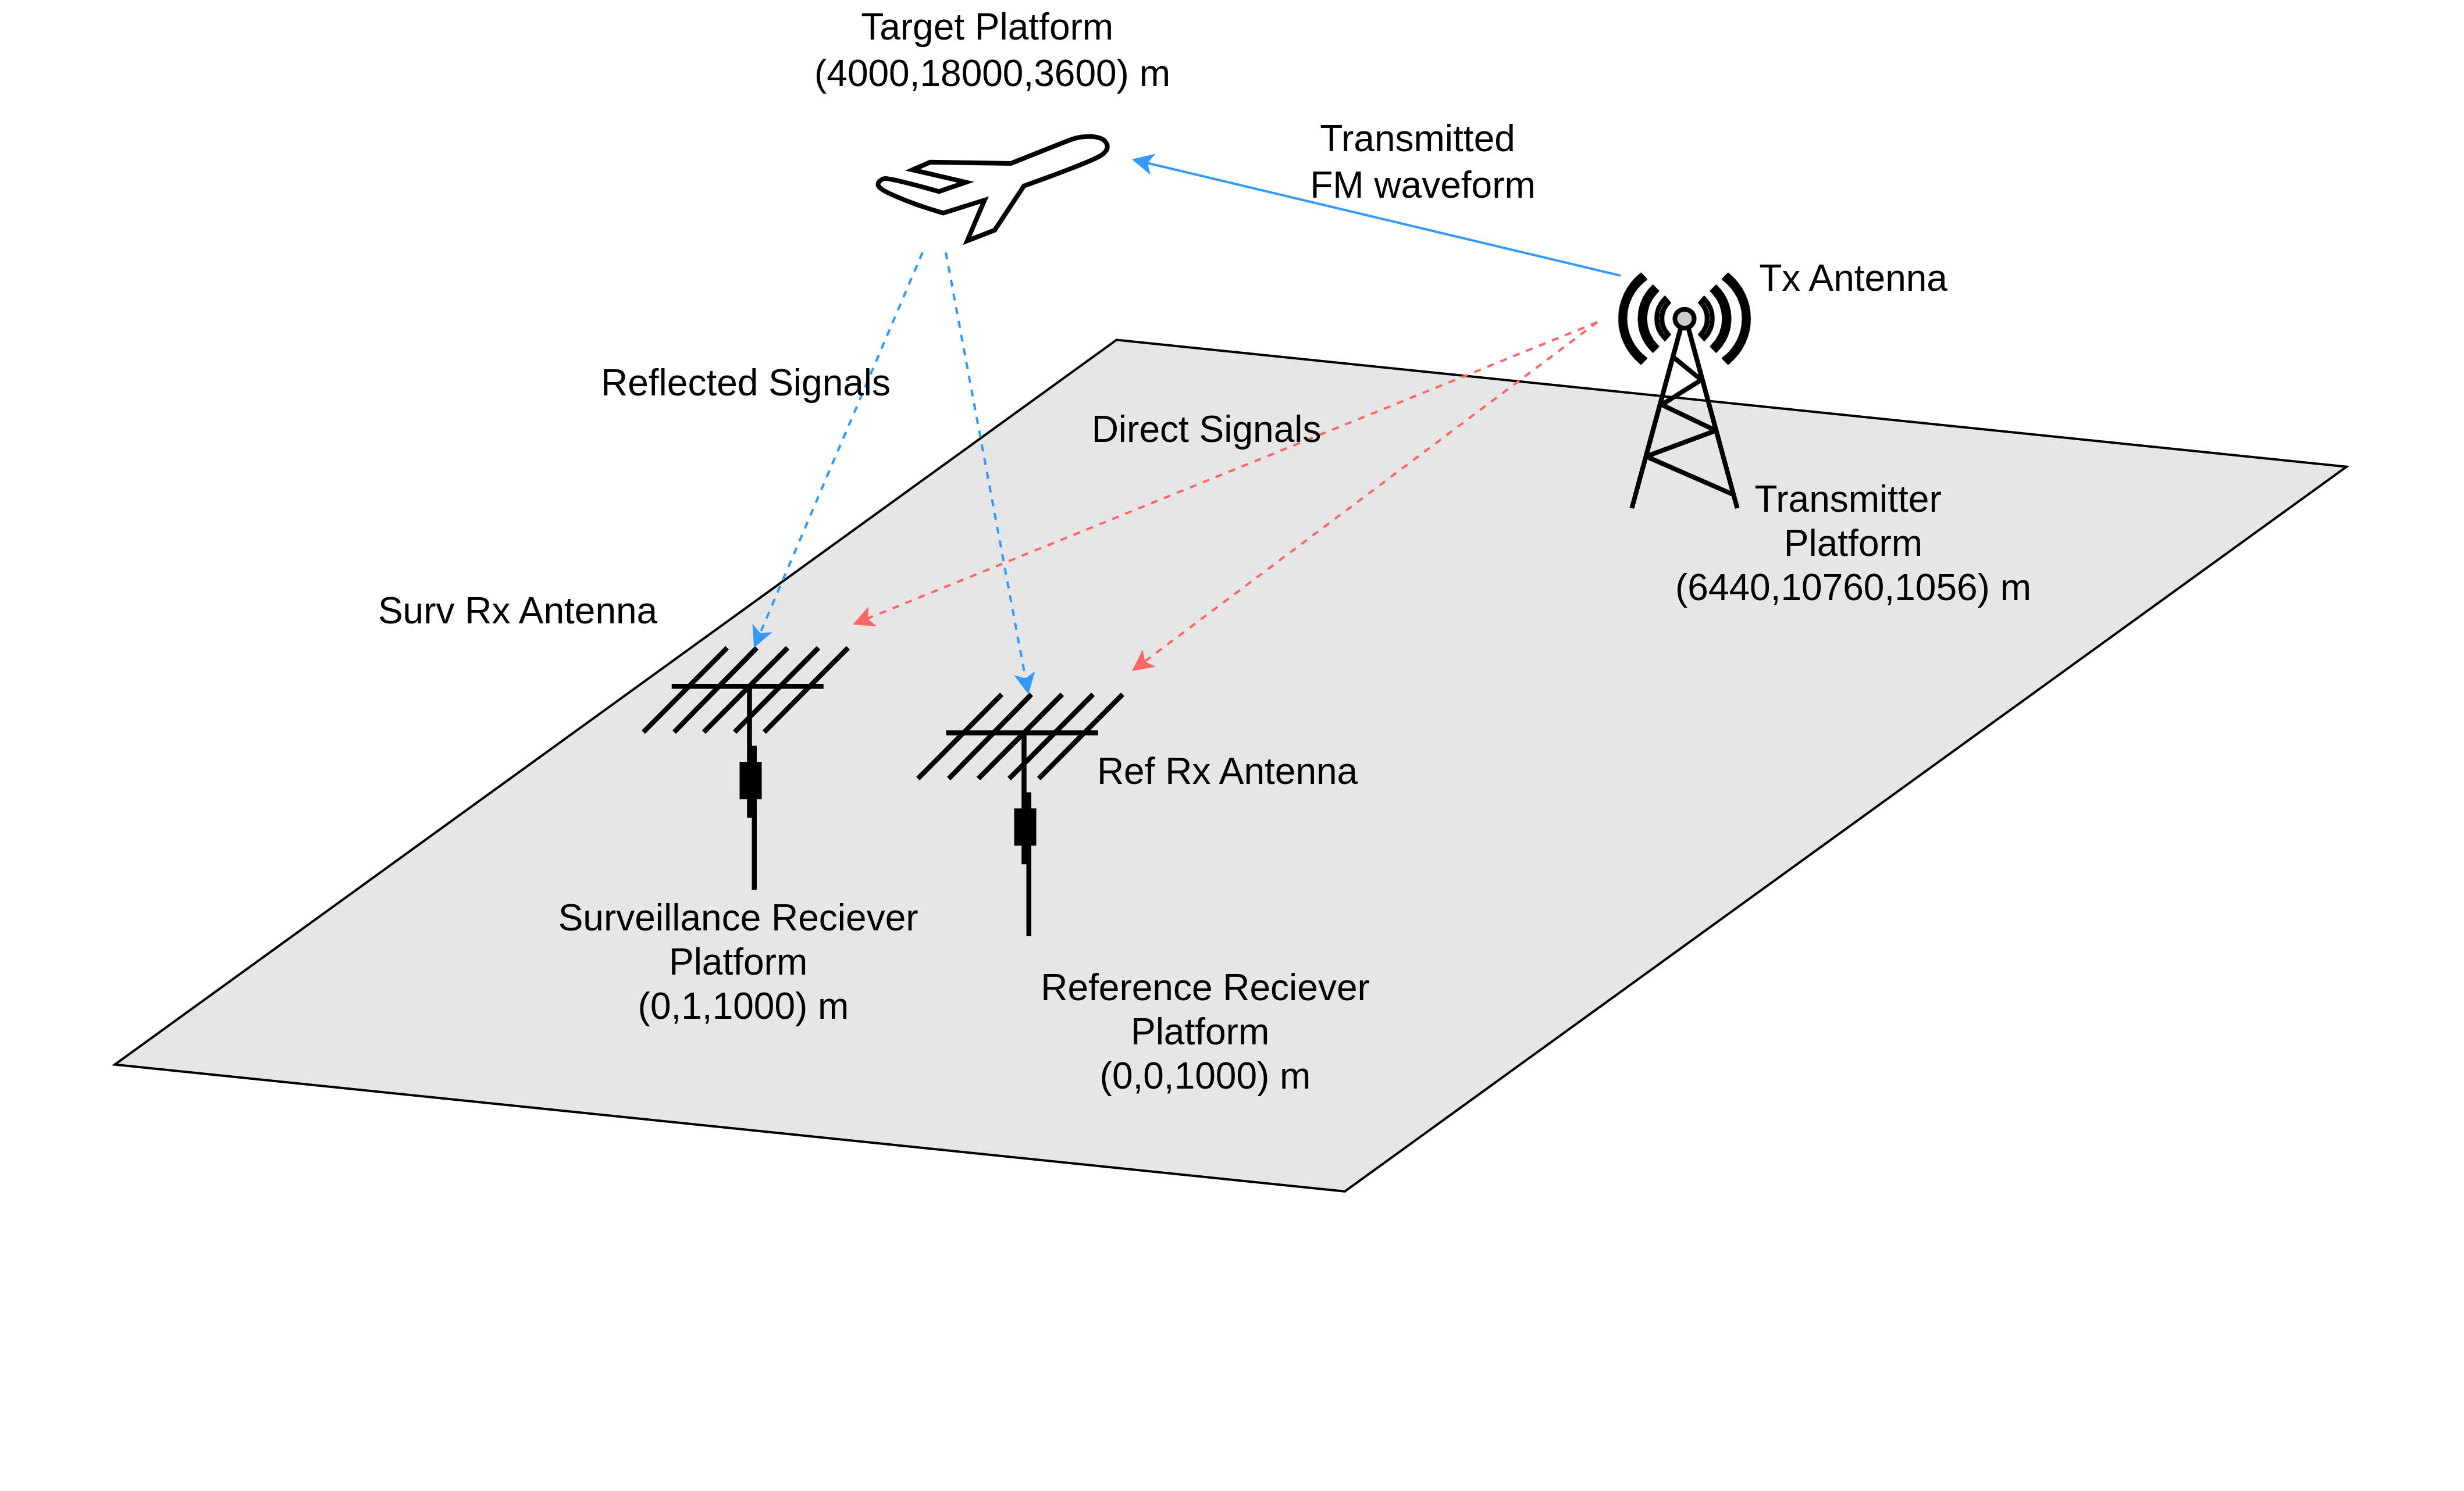
\includegraphics[width=0.85\linewidth]{Figure/fersBistaticRadar.drawio (3).png}
    \caption{Geometry of the Bistatic Radar in the FERS Simulation with the target in its initial position.}
    \label{fig:ferssetup}
\end{figure}
%%Corrections from Feeback [15]
The target is simulated as a single aircraft following a straight 
flight path, defined by Cartesian waypoints interpolated using cubic splines 
in MATLAB. The trajectory and corresponding ground truth data are shown in 
Figure \ref{fig:ard1setup}.
\newline
\begin{figure}[h!]
    \centering
    \begin{subfigure}[b]{0.49\linewidth}
        \centering
        \includesvg[width=\linewidth,inkscapelatex=false]{Figure/basicFersScenarioTargetPath.svg}
    \end{subfigure}
    \hfill
    \begin{subfigure}[b]{0.45\linewidth}
        \centering
        \includesvg[width=\linewidth,inkscapelatex=false]{Figure/basicFERS_ScenarioGroundTruth.svg}
    \end{subfigure}
    \caption{The basic FERS simulation scenario. Left: Target trajectory for 
    the straight and level flight scenario in Cartesian coordinates. Right: 
    Ground truth bistatic range and Doppler shift computed from the 
    simulated target coordinates at each time step.}
    \label{fig:ard1setup}
\end{figure}
%%%%%%%%%%%%%%%%%%%%%%%%%%%%%%%%%%%%%%
%%%%%%%%%%%%%%%%%%%%%%%%%%%%%%%%%%%%%%

The bistatic range and Doppler processing utilizes a set of 200 kilosamples, determined by the configured sampling rate in \ac{FERS}. The \ac{ARD} response output observed in Figure \ref{fig:ambiguityFunction} is taken after 2 seconds of sampling data. The resulting \ac{ARD} shown in Figure \ref{fig:ambiguityFunction}  exhibits a distinctive peak at a bistatic Doppler shift of 0 Hz. The peak at 0 Hz, strongest near zero range, indicates \ac{DPI}, likely due to signal leakage into the surveillance channel. Additional peaks at similar ranges to the \ac{DPI} are sidelobes of the \ac{FM} waveform's ambiguity function, further obscuring the target, it can be observed that the returns from the \ac{DPI} complicate target resolution.

\begin{figure}[H]
    \centering
    \includesvg[width=0.9\linewidth]{Figure/ardMapFinal.svg}
    \caption{Amplitude/Range/Doppler map.}
    \label{fig:ambiguityFunction}
\end{figure}
Although the cross-correlation function enhances processing gains, it also amplifies DPI and clutter which is undesired, leading to side-lobes that often mask target returns, as observed in Figure \ref{fig:ambiguityFunction}. The following subsection will discuss the application of a DPI cancellation algorithm for suppressing the \ac{DPI} and clutter.

%Range Smearing and side lobes

\subsection{Direct Path Interference and Clutter Suppression}
To improve the probability of detection, it is essential to suppress \ac{DPI} and clutter from the surveillance channel. This suppression is performed directly on the surveillance signal before the range and Doppler Processing stage. For this purpose, the \ac{ECA} which uses the least mean squares estimator technique is applied. The \ac{ECA}, as proposed by Colone \textit{et al.}\cite{coloneECA}, is recognized for its fast convergence and not requiring any tuning \cite{OHagan2008, tong2014}. Notably, in 2007 Cardinali \textit{et al.} conducted a comparative study of various \ac{DPI} cancellation algorithms, demonstrating the superior performance of the \ac{ECA} in achieving nearly complete clutter suppression, despite its higher computational demands compared to the other algorithms \cite{cardinali2007comparison,Heunis2010}. The \ac{ECA} is therefore selected for its proven effectiveness in mitigating clutter and \ac{DPI}. The focus here is on validating the results of this algorithm to ensure it operates as expected. The \ac{ARD} plot in \ac{2D} is shown before and after the DPI and clutter cancellation at \(t=2\)s in figures \ref{fig:ardDPIbefore} and \ref{fig:ardDPIAfter} respectively.

\begin{figure}[H]
    \centering
    \includesvg[width=0.8\linewidth,inkscapelatex=false]{Figure/ardBeforeDPI_unnormalized_correction1.svg}
    \caption{Amplitude/Range/Doppler map before DPI and clutter cancellation.}
    \label{fig:ardDPIbefore}
\end{figure}
\begin{figure}[H]
    \centering
    \includesvg[width=0.8\linewidth,inkscapelatex=false]{Figure/ardFinalAfter_correction1.svg}
    \caption{Amplitude/Range/Doppler map after DPI and clutter cancellation. The line at 0 Hz bistatic Doppler frequency indicates zero Doppler cancellation. The black circle marking illustrates the  target that  appears at a Doppler frequency of around 147 Hz.}
    \label{fig:ardDPIAfter}
\end{figure}

The range and Doppler map reveal the target more clearly after applying the \ac{ECA} algorithm, with the target observed at a bistatic Doppler frequency of around 147 Hz. Notably, the line at zero bistatic Doppler frequency shows a significantly reduced amplitude, illustrating the strong cancellation of zero Doppler components and demonstrating the effectiveness of the \ac{DPI} cancellation.

\subsection{Target Detection}
The Target Detection stage is responsible for identifying potential targets from the \ac{ARD} map. Using the range and Doppler response plots discussed in the previous subsections, this stage involves evaluating each cell in the range and Doppler domain against some threshold. This threshold is typically determined based on the values of the surrounding cells to effectively distinguish targets from background noise. One of the common effective implementations is the use of a \ac{CFAR} filter. This method provides the capability to tune the probability of detection \(p_d\) by varying the probability of false alarm \(P_{fa}\).


%Motivation for CA CFAR
In \ac{Radar} signal processing, various algorithms are designed for adaptive thresholding to achieve a \ac{CFAR}. 
These algorithms include, but are not limited to, \ac{CA-CFAR}, \ac{OSGO-CFAR}, \ac{VI-CFAR}, \ac{OS-CFAR}, \ac{SO-CFAR}, and \ac{GO-CFAR} \cite{hatem2018comparative}. In this research, the \ac{CA-CFAR} algorithm is used for target detection due to its simplicity and lower complexity compared to the other \ac{CFAR} algorithms. The \ac{CA-CFAR} has been effectively used in conjunction with similar algorithms used in this research, such as the \ac{ECA} for detection in \ac{PR} systems \cite{Colone2009,Golabi2013}.

\subsubsection{Cell-Averaging CFAR}
The \ac{CFAR} filter's function is to establish the power threshold, beyond which any detected echo is likely to be from a target. If this threshold is set too low, it will result in more echoes being detected, leading to an increase in false alarms \cite{Shrivathsa2008a}. In the \ac{CA-CFAR} case this is achieved by averaging the output over the adjacent cells to compute the threshold.
\begin{figure}[H]
    \centering
    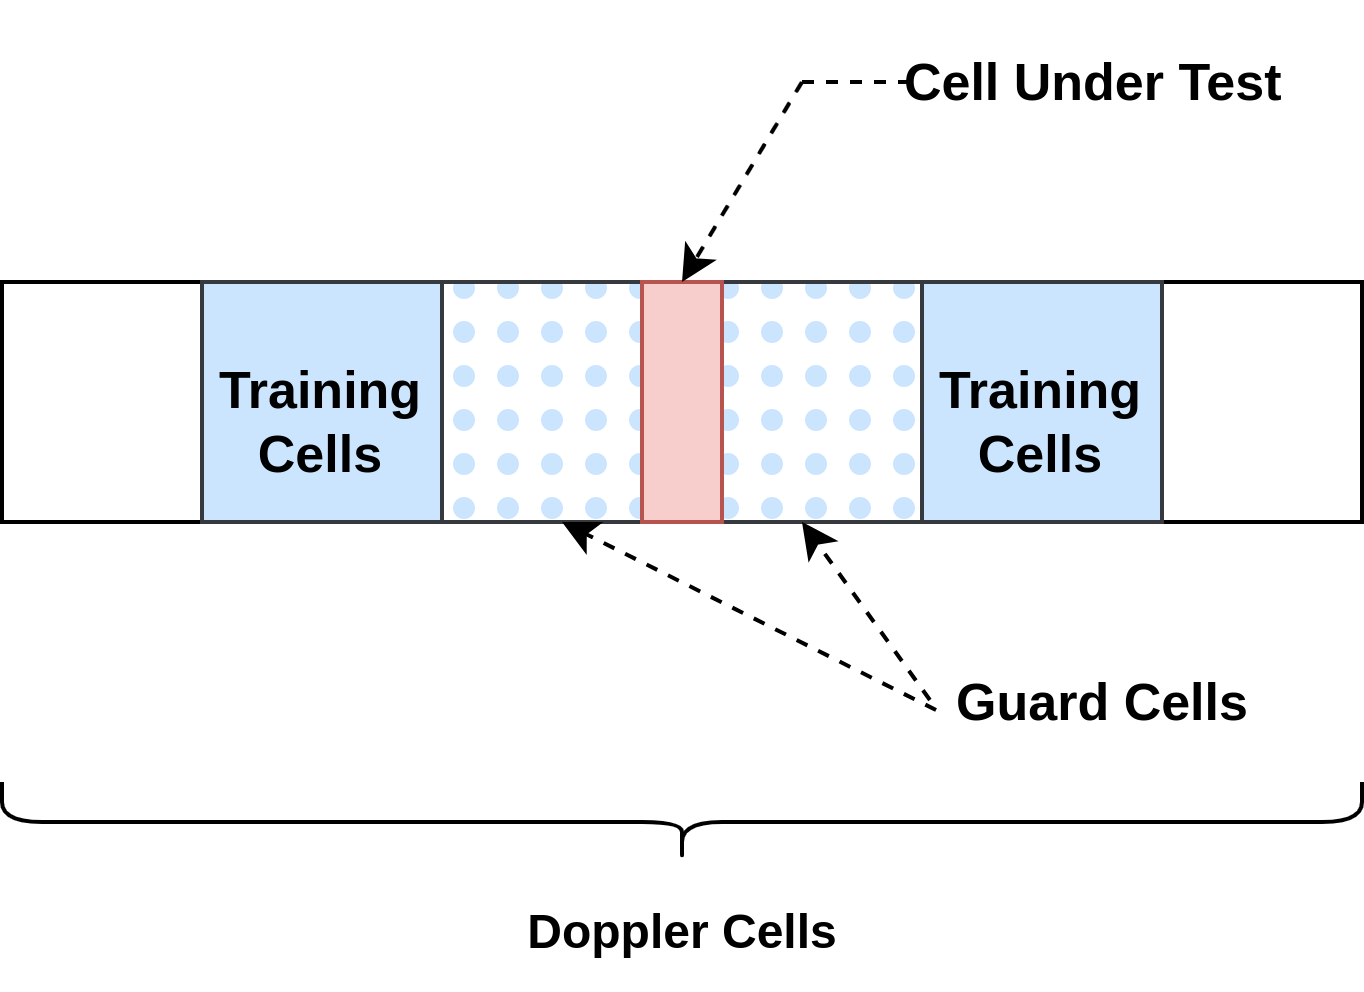
\includegraphics[width=0.55\linewidth]{Figure/cacfar.drawio.png}
    \caption{Cell-Averaging CFAR principle.}
    \label{fig:cacfar}
\end{figure}
%Norman Pearson Detector
The basic principle of the \ac{CA-CFAR} algorithm is illustrated in Figure \ref{fig:cacfar}. In this method, the adjacent cells to the \ac{CUT} are designated as guard cells. The selection of these guard cells depends on the expected number of cells to be occupied by the target in the range or Doppler domain, which is influenced by the \ac{Radar}’s resolution capabilities. Training cells, located around the \ac{CUT}, are used to dynamically compute the average noise power. This average is then scaled by a factor \(\alpha\) to determine the threshold for target detection, as shown in Equation (\ref{thresholdCFAR}). If the power level in the \ac{CUT} exceeds this threshold, a target is detected.

The noise power \(P_n\) from the neighboring cells is scaled by the factor \(\alpha\) \cite{Shrivathsa2008a}:
\begin{equation}
    T = \alpha \cdot P_n
    \label{thresholdCFAR}
\end{equation}

To compute \(P_n\) the  power levels from the training cells are averaged, where \(x_m\) represents the power level in the \(m\)-th cell and \(N\) is the number of training cells as shown in Equation (\ref{thresholdCFAR}):

\begin{equation}
    P_n = \frac{1}{N} \sum_{m=1}^N x_m
\end{equation}
\newline
\newline
The scaling factor is computed according to Equation (\ref{alpha}) where \(P_{fa}\) is the desired probability of false alarm  \cite{Sambath2020a} :

\begin{equation}
    \alpha = N \cdot (P_{fa}^{-\frac{1}{N}}-1)
    \label{alpha}
\end{equation}
%NB - make other references to range smearing
In the range and Doppler plots discussed in the previous subsection, it is observed that the target spans across multiple range bins. This is a common issue when using \ac{FM} transmitted waveform due to low bandwidth, coupled with the instantaneous bandwidth due to the inconsistencies in the broadcasted audio signal, which can cause fluctuations in the range resolution (\(\delta R = c/2B\)), leading to range smearing. This makes setting the number of guard and reference cells in range dimension challenging. Consequently, averaging is then performed only in the bistatic Doppler domain, where higher Doppler resolution is available. The \ac{CA-CFAR} parameters used are presented in Table \ref{tab:cacfartable}.

\begin{table}[ht!]
\centering
\caption{CA-CFAR Parameters.}
\label{tab:cacfartable}
\begin{tabular}{ll}
\hline
\textbf{Parameter} & \textbf{Value} \\
\toprule
\(P_{fa}\)  & \(10^{-5}\) \\
Doppler Training Cells & 6  \\
Doppler Guard Cells  & 4 \\
\bottomrule
\end{tabular}
\end{table}
 The \(P_{fa}\)  was selected through a systematic sensitivity analysis, the results of which are illustrated in Figure~\ref{fig:cfarValidation}, which presents a range-Doppler line cut at a bistatic range of 15~km. Lower \(P_{fa}\)  values produced thresholds approaching the noise floor, increasing susceptibility to false alarms, while higher values elevated the threshold above the target return, risking target suppression. A \(P_{fa}\) value of \(10^{-5}\)  was therefore selected as it provided the most favourable balance between detection sensitivity and false alarm suppression. The \ac{CA-CFAR} was used with 4 guard cells and 6 training cells on both sides of the \ac{CUT}, similar to the approach followed in \cite{De2015,tong2014}. Figure \ref{cfarwindow} shows the CFAR window.
\newline
\begin{figure}[H]
    \centering
    \includesvg[width=1\linewidth]{Figure/cfar_ca.drawio.svg}
    \caption{CFAR window with 21 cells.}
    \label{cfarwindow}
\end{figure}
Using the parameters listed in Table \ref{tab:cacfartable}, the \ac{CA-CFAR} is applied on the range and Doppler map and the output is shown in Figure \ref{fig:ca-cfar1}.
%false alarm ??
\begin{figure}[H]
    \centering
    \includesvg[width=0.7\linewidth,inkscapelatex=false]{Figure/cacfar_pfa5_corrections.svg}
    \caption{CA-CFAR output with \(P_{fa}\) of \(10^{-5}\): The Target is observed at around a bistatic Doppler frequency of 147 Hz.}
    \label{fig:ca-cfar1}
\end{figure}

\begin{figure}[H]
    \centering
    \includesvg[width=0.7\linewidth,inkscapelatex=false]{Figure/cacfar_pfa7_correction.svg}
    \caption{CA-CFAR output with \(P_{fa}\) of \(10^{-7}\): A decrease in the number of observations is observed due to the decrease in \(P_{fa}\).}
    \label{fig:ca-cfar2}
\end{figure}

To validate the accuracy of the dynamic threshold and the functionality of the \ac{CA-CFAR} filter, the bistatic Doppler response and the threshold are computed at a specific bistatic range with different \(P_{fa}\) where the target is present, as shown in Figure \ref{fig:cfarValidation}.

\begin{figure}[H]
    \centering
    \includesvg[width=0.9\linewidth,inkscapelatex=false]{Figure/ca_cfar_validate_corrections_v2.svg}
    \caption{CA-CFAR output with the threshold value at a bistatic range of 15 km with a \(P_{fa}\) of \(10^{-3}\) to \(10^{-7}\).}
    \label{fig:cfarValidation}
\end{figure}



\subsubsection{Target  Centroids}
The \ac{CFAR} outputs presented in the previous subsection, show multiple detections across various  Doppler and range cells. To effectively use these detections in tracking filters, additional processing is necessary to group the detections into clusters and extract target coordinates. Each cluster represents a distinct target, and the extracted centroids will serve as measurements for tracking filters. Identifying distinct targets from a \ac{CFAR} output usually involves a robust clustering algorithm to group the bistatic range and Doppler cells associated with each target.

Various clustering techniques have been used throughout the literature for post-processing CFAR detections. For instance, in \cite{kuang2020applied}, the K-means clustering algorithm is used to derive target centres from \ac{CFAR} outputs. Additionally, \ac{DBSCAN} has been used to identify clusters in \ac{CFAR} detections, as demonstrated in \cite{li2024density,schubert2015clustering}. Mean-shift clustering, a well-known density-based method, differs from K-means in that it does not require prior knowledge of the number of clusters or assumptions about their shapes. While \ac{DBSCAN} can identify clusters, additional processing is required to compute the mean of the points in each cluster to extract the centroids. In contrast, mean-shift clustering relies solely on an estimated bandwidth size to group detections, as outlined in \cite{derpanis2005mean}. Consequently, the mean-shift algorithm is used here to directly produce target centroids from \ac{CFAR} outputs.
\newline
\newline
%Clustering
Mean-shift clustering is an iterative algorithm that shifts each data point toward regions of higher density in the feature space \cite{cheng1995mean}. It does so by moving each point to the mean of points within a specified bandwidth. This process continues until convergence, forming clusters as points gather around high-density regions. The kernel used, typically a Gaussian kernel, determines how weights are applied within the bandwidth, influencing the direction and magnitude of the shift \cite{cariou2022novel}. This results in a set of cluster centroids representing the densest areas in the data. The mean-shift clustering algorithm is discussed extensively in the literature \cite{cariou2022novel,wu2007mean}, with the focus here being on validating its results. The algorithm used is illustrated in algorithm \ref{alg:mean_shift}, adapted from \cite{carreira2015review}. 
\newline 
\newline
\begin{figure}[H]
    \centering
    \includesvg[width=0.7\linewidth,inkscapelatex=false]{Figure/cacfar_pfa7_centroid_correction.svg}
    \caption{CFAR output with centroids.}
    \label{fig:cfar_centers}
\end{figure}
The bandwidth parameter used in the mean-shift clustering algorithm for the bistatic Doppler and bistatic range measurements is selected as \( \sigma = [5 \, \text{Hz}, 10 \, \text{km}] \) respectively. Detections falling within this kernel bandwidth are considered part of the same neighbourhood. This parameter defines the neighbourhood size around each data point used for calculating the mean shift \cite{Wu2007}. Figure \ref{fig:cfar_centers} shows the clusters detected in the \ac{CFAR} output, with the centroids of each cluster highlighted as red squares. A drawback of this approach is that if target detections are closely spaced in both bistatic range and Doppler, they may be clustered into a single detection.\footnote{A video showing the \ac{CA-CFAR} with a \(P_{fa}\) of \(10^{-5}\) and Mean-Shift clustering outputs for a single target can be found at: \url{https://youtu.be/nWzsm2Biv8Y}. The Matlab code for the implementation of Mean-shift Algorithm and the \ac{CA-CFAR} can be found in the code repository from Appendix \ref{appendix:repo}.}
\newline 
\begin{algorithm}[H]
\caption{Mean-shift Clustering}
\label{alg:mean_shift}
\begin{algorithmic}[1]
    \vspace{2em}
    \State \textbf{Initialize:}
    \vspace{0.3em}
    \Statex $\text{dataPoints} \gets \text{input data}$
    \Statex $\text{bandWidthX} \gets \text{bandWidthX}$
    \Statex $\text{bandWidthY} \gets \text{bandWidthY}$
    \Statex $\text{stopThresh} \gets 1e{-3} \times [\text{bandWidthX}, \text{bandWidthY}]$
    \Statex $\text{clusterCentroids} \gets [\,]$
    \vspace{1em}
    
    \State \textbf{Main Loop:}
    \vspace{1em}
    \While{$\text{numInitPts} > 0$}
        \State $\text{startPt} \gets \text{randomly select a point from initial Points}$
        \State $\text{mean} \gets \text{dataPoints[:, startPt]}$
        \vspace{0.5em}
        \While{not converged}
            \State $\text{sqDistToAll} \gets \frac{(\text{mean}(1)-\text{dataPoints}(1,:))^2}{\text{bandWidthX}} + \frac{(\text{mean}(2)-\text{dataPoints}(2,:))^2}{\text{bandWidthY}}$
            \vspace{0.5em}
            \State $\text{weights} \gets \exp\left(-\frac{1}{2} \times \text{sqDistToAll}\right)$
            \vspace{0.5em}
            \State $\text{newMean} \gets \frac{\sum (\text{weights} \times \text{dataPoints}[:, :])}{\sum \text{weights}}$
            \vspace{0.5em}
            \State $\text{Members} \gets [\text{Members}, \text{find}(\text{sqDistToAll} < 1)]$
            \vspace{0.5em}
            \State $\text{beenVisitedFlag}[\text{Members}] \gets 1$
            \vspace{0.5em}
            \If{$\text{norm}(\text{newMean} - \text{mean}) < \text{stopThresh}$}
                \State Check for merge possibilities
                \vspace{0.5em}
                \If{merge found}
                    \State Merge clusters
                \Else
                    \State Create new cluster
                \EndIf
                \State \textbf{break}
            \EndIf
            \vspace{0.5em}
            \State $\text{mean} \gets \text{newMean}$
        \EndWhile
        \vspace{0.5em}
        \State \text{Update clusters and initial Points}
    \EndWhile
    \vspace{1em}
\end{algorithmic}
\end{algorithm}

\newpage
\section{Target Modelling}

The centroids from the clustering process, are used to estimate the target's position in the bistatic range and Doppler domain. To accurately estimate the target's state, it is required to model the target's motion. Target motion models are typically classified as either manoeuvring or non-manoeuvring  in tracking problems \cite{Li2003a}. For our tracking scenarios, a non-maneuvering target, such as a commercial aircraft, is expected in the bistatic Doppler and range domain, where abrupt changes in the bistatic range or Doppler are unlikely. Therefore, a \ac{NCV} model is used, similar to \cite{Boyer2012} which assumes a nearly constant velocity between the sampling interval.

\subsection{Nearly-Constant Velocity Model}
The target's motion in a \ac{2D} Cartesian coordinate system with constant velocity can be modelled by the state vector \( [x, \dot{x}, y, \dot{y}] \), where \( x \) and \( y \) represent positions, and \( \dot{x} \) and \( \dot{y} \) represent velocities. Similarly, the state of the target in the bistatic range and Doppler domain is modelled by the bistatic range, bistatic range rate, bistatic Doppler, and bistatic Doppler rate, as shown in  Equation (\ref{stateEq}):

\begin{equation}
    x(t) = [r_t, \dot{r}, f_t, \dot{f_t}]^T
    \label{stateEq}
\end{equation}

where \(r_t\) is the bistatic range, \(f_t\) is the bistatic Doppler, \(\dot{r_t}\) and \(\dot{f_t}\) are bistatic range rate and bistatic Doppler rate respectively in continuous time. The \ac{NCV} model is represented as:

\begin{equation}
    \mathbf{X}_k = 
    \begin{bmatrix}
        1 & \tau & 0 & 0 \\
        0 & 1 & 0 & 0 \\
        0 & 0 & 1 & \tau \\
        0 & 0 & 0 & 1 \\
    \end{bmatrix} X_{k-1} + w_{k-1}
\end{equation}

where, \( \tau \) is the sampling interval, and \( w_{k-1} \) is the discrete white acceleration noise. This noise accounts for small, random variations in acceleration that cannot be predicted \cite{Li2003a}. Assuming a discrete-time model with zero-mean white Gaussian noise characterized by the covariance matrix \( Q \):

\begin{equation}
    Q = \text{cov}(w_k) = S_w \tilde{Q},
\end{equation}

where:

\begin{equation}
    \tilde{Q}  = \begin{bmatrix}
        \tau^4/4 & \tau^3/2 & 0 & 0 \\
        \tau^3/2 & \tau^2 & 0 & 0 \\
        0 & 0 & \tau^4/4 & \tau^3/2\\
        0 & 0 & \tau^3/2 & \tau^2\\
    \end{bmatrix}
    \label{Qmatrix}
\end{equation}

\( S_w \) represents the process noise power spectral density \cite{Measurements2023b}. The white acceleration model can also be adapted for tracking manoeuvring targets by using the manoeuvring index \( \lambda \) defined as:

\begin{equation}
    \lambda = \frac{\sqrt{S_w \tau^3}}{\sigma_r}, 
\end{equation}

where \( \lambda \) is the ratio of the \ac{RMS} motion uncertainty to the measurement uncertainty. Lower values of \( S_w \) describe a \ac{NCV} model, while higher values correspond to a manoeuvring target model \cite{953264}.


\section{Tracking Filters Implementation}

This section describes the implementation of the tracking filters introduced in Chapter 3. The filters are used to track targets based on observations from the target detections. A basic scenario with a simulated target in the FERS framework is used to demonstrate the functionality of the four filters. The target is simulated in the same bistatic radar geometric setup 
from Figure \ref{fig:ferssetup}. The trajectory and corresponding ground 
truth data are shown in Figures \ref{fig:targetpath2} and 
\ref{fig:groundtruth2} respectively. The performance and investigation of 
the filters' optimal parameters are discussed in the next chapter.

\begin{figure}[H]
    \centering
    \includesvg[width=0.7\linewidth,inkscapelatex=false]{Figure/basicFersScenarioTargetPath2.svg}
    \caption{Target trajectory for the flight scenario in Cartesian 
    coordinates.}
    \label{fig:targetpath2}
\end{figure}

\begin{figure}[H]
    \centering
    \includesvg[width=0.55\linewidth,inkscapelatex=false]{Figure/basicFERS_ScenarioGroundTruth2.svg}
    \caption{Ground truth bistatic range and Doppler shift computed from 
    the simulated target coordinates at each time step.}
    \label{fig:groundtruth2}
\end{figure}%feedback 15
\subsection{Kalman Filter}
The Kalman Filter is implemented using the algorithm shown in Algorithm \ref{alg:kalman_filter}. The parameters that need to be initialized include the initial state estimate \(x_0\), the initial error covariance matrix \(P_0\), the process noise covariance matrix \(Q\), and the measurement noise covariance matrix \(R\). The first detection of the target is used to initialize the state vector \(x_0\).

\textbf{Initial Error Covariance Matrix:}
\newline
The initial error covariance matrix, as discussed in Section 3, models the uncertainty in the state estimate. The error covariance matrix is updated in each prediction-update cycle of the Kalman Filter. It is initialized according to the expected uncertainty values, similar to the approach followed by Howland \cite{Howland2005a}:
\begin{equation}
    P_0 = \begin{bmatrix}
        5 & 0 & 0 & 0 \\
        0 & 0.04 & 0 & 0 \\
        0 & 0 & 0.0225 & 0 \\
        0 & 0 & 0 & 0.1 \\
    \end{bmatrix}
\end{equation}


\textbf{Measurement Error Covariance Matrix:}
\newline
The measurement error covariance matrix, defined in Equation (\ref{measurement_eq}), is selected based on the expected standard deviation of the measurement errors in the bistatic range and Doppler domains:

\begin{equation}
    R = \begin{bmatrix}
        \sigma_{\text{range}}^2 & 0 \\
        0 & \sigma_{\text{doppler}}^2 \\
    \end{bmatrix}
\end{equation}

The measurement covariance matrix values were determined by analysing the observed deviations in the bistatic range and Doppler domain. The bistatic range standard deviation, \(\sigma_{\text{range}} = 1\) km, was obtained from the standard deviation of errors between simulated and ground truth data. Similarly, the Doppler shift standard deviation, \(\sigma_{\text{doppler}} = 0.1\) Hz, was obtained from observed deviations in Doppler measurements. This approach aligns with \cite{De2015}, where standard deviations from field deployment data were used to define the measurement covariance matrix.  

\textbf{Process Noise Covariance Matrix:}
\newline
The process noise covariance matrix is defined by the Equation in (\ref{Qmat}), where \(S_w = [s_{w1}, s_{w2}]\) represents the process noise power spectral densities for the bistatic range and Doppler, respectively:
\begin{equation}
    Q  = \begin{bmatrix}
        \frac{\tau^4}{4} s_{w1} & \frac{\tau^3}{2} s_{w1} & 0 & 0 \\
        \frac{\tau^3}{2} s_{w1} & \tau^2 s_{w1} & 0 & 0 \\
        0 & 0 & \frac{\tau^4}{4} s_{w2} & \frac{\tau^3}{2} s_{w2} \\
        0 & 0 & \frac{\tau^3}{2} s_{w2} & \tau^2 s_{w2} \\
    \end{bmatrix}
    \label{Qmat}
\end{equation}

The values of \(s_{w1}  \) and \(s_{w2}\) are determined through a tuning process and their effect is demonstrated in Figure \ref{kalman_results1}.
\begin{figure}[H]
    \centering
    \begin{subfigure}[b]{0.49\linewidth}
        \centering
        \includesvg[height=6cm,inkscapelatex=false]{Figure/kf_R_corrections_v1.svg}
        \caption{Kalman Filter with different values for \(\sigma_{range}\) and \(\sigma_{doppler}\).}
        \label{kalman_results}
    \end{subfigure}
    \hfill
    \begin{subfigure}[b]{0.49\linewidth}
        \centering
        \includesvg[height=6cm,inkscapelatex=false]{Figure/kf_SW_corrections_v1.svg}
        \caption{Kalman Filter with different values for \(s_{w1}\) and \(s_{w2}\) for the \(Q\) covariance matrix.}
        \label{kalman_results1}
    \end{subfigure}
    \caption{ Kalman Filter with varying measurement and process noise covariance matrices.}
\end{figure}

A single target is configured in \ac{FERS} using the geometric setup in Figure \ref{fig:ferssetup} and the target path in Figure \ref{fig:targetpath2}. The results for the basic scenario in \ac{FERS} using the Kalman Filter are presented in figures \ref{kalman_results} and \ref{kalman_results1}.
\newline
% Added cumulative error metric and two new figures
\begin{figure}[H]
    \centering
    \begin{subfigure}[b]{0.49\linewidth}
        \centering
        \includesvg[width=\linewidth,inkscapelatex=false]{Figure/KF_R_CumSum.svg}
        \caption{Kalman Filter Cumulative Error with different values for \(\sigma_{range}\) and \(\sigma_{doppler}\).}
        \label{kalman_results_cum}
    \end{subfigure}
    \hfill
    \begin{subfigure}[b]{0.49\linewidth}
        \centering
        \includesvg[width=\linewidth,inkscapelatex=false]{Figure/KF_Q_CumSum.svg}
        \caption{Kalman Filter Cumulative Error with different values for \(s_{w1}\) and \(s_{w2}\) for the \(Q\) covariance matrix.}
        \label{kalman_results_cum1}
    \end{subfigure}
    \caption{ Kalman Filter Cumulative Error with varying measurement and process noise covariance matrices.}
\end{figure}
To provide a quantitative assessment of the sensitivity of the Kalman Filter to the covariance matrices $\mathbf{R}$ and $\mathbf{Q}$, a cumulative error metric was computed relative to the ground truth trajectory. The cumulative error is defined as the sum of the Euclidean distance between the estimated and true target positions over the duration of the simulation. The resulting cumulative errors for different parameter configurations are shown in Figures \ref{kalman_results_cum} and \ref{kalman_results_cum1}.

The behaviour of a tracking filter is highly influenced by the process noise covariance matrix $\mathbf{Q}$ and the measurement noise covariance matrix $\mathbf{R}$. As shown in Figure \ref{kalman_results}, increasing the values in $\mathbf{R}$ results in less precise predictions, with the filter giving more weight to the process model rather than the measurements. This leads to predictions that are more loosely constrained, as expected. Similarly, Figure \ref{kalman_results1} demonstrates the impact of increasing the process noise power spectral density. The cumulative error results shown in Figures \ref{kalman_results_cum} and \ref{kalman_results_cum1} also provide a quantitative confirmation of these effects. Higher values lead to a larger process noise covariance matrix, causing the predicted state estimates to become more dispersed, reflecting the increased uncertainty in the system's dynamics. This confirms the significant impact that both the $\mathbf{R}$ and $\mathbf{Q}$ covariance matrices have on estimating dynamic states as noted in \cite{Akhlaghi2018}.



\subsection{Unscented Kalman Filter}
Similar to the Kalman Filter, the matrices \(P\), \(R\), \(Q\), and the state vector \(x_0\) are initialized in the same way. However, additional parameters are required for the \ac{UKF}, as shown in Table \ref{tab:ukf_params}.
\begin{table}[H]
    \centering
    \large
    \caption{Parameters Used for Unscented Kalman Filter.}
    \label{tab:ukf_params}
    \begin{tabular}{ll}
        \toprule
        Parameter & Value \\
        \midrule
        \( n \) & 4 \\
        \( \alpha \) & 0.01 \\
        \( \kappa \) & 0 \\
        \( \beta \) & 2 \\
        \bottomrule
    \end{tabular}
\end{table}
The \ac{UKF} includes parameters \(\alpha\), \(\beta\), \(\kappa\), and \(n\), where \(\alpha\) controls the dispersion of sigma points relative to the state vector's mean, 
\(\kappa\) functions as an additional scaling factor, and \(\beta\) integrates prior information 
about the input random variable's distribution \cite{Cai2006}. The parameter \(n\) represents the dimension of the state vector. The value of \(\beta\) is typically chosen as 2, which is considered optimal, and \(\kappa\) is usually set to 0 \cite{Cai2006}. \(\alpha\) is generally set to a small value such as \(1 \times 10^{-3}\), and in this case, it was determined by varying the parameter and observing its impact, as demonstrated in Figure \ref{tab:ukf_params}.
 \newline
 \newline
The results of the \ac{UKF} tracking are presented in \ref{ukfres} and \ref{ukfres2} where different \ac{UKF} parameters for \(\alpha\) and \(\beta\) were used.
\begin{figure}[ht!]
    \centering
    \begin{subfigure}[b]{0.48\linewidth}
        \centering
        \includesvg[height=6cm,inkscapelatex=false]{Figure/ukf_alpha_v3.svg}
        \caption{UKF with different values for alpha.}
        \label{ukfres}
    \end{subfigure}
    \hfill
    \begin{subfigure}[b]{0.48\linewidth}
        \centering
        \includesvg[height=6cm,inkscapelatex=false]{Figure/ukf_beta_v3.svg}
        \caption{UKF with different values for beta.}
        \label{ukfres2}
    \end{subfigure}
    \caption{UKF with varying values of \(\alpha\) and \(\beta\).}
\end{figure}
As shown in Figure \ref{ukfres}, the impact of the \(\alpha\) parameter on the filter's estimations is evident. This is consistent with the role of \(\alpha\), which affects how the sigma points are spread around the mean of the state vector \cite{Cai2006}. For smaller values of \(\alpha\), the mean state estimate becomes more dispersed, leading to noticeable deviations in the filter estimates. As expected, the \(\beta\) parameter does not show any observable effect on the filter's estimations due to its minimal impact on the performance of the filter.
\newline
%%%%%%%%% Added cumulative error metric and two new figures %%%%%%%%%%%%
\begin{figure}[ht!]
    \centering
    \begin{subfigure}[b]{0.48\linewidth}
        \centering
        \includesvg[width=\linewidth,,inkscapelatex=false]{Figure/UKF_AlphaCumError.svg}
        \caption{\ac{UKF} Cumulative Error with different values for alpha.}
        \label{ukfresCumError}
    \end{subfigure}
    \hfill
    \begin{subfigure}[b]{0.48\linewidth}
        \centering
        \includesvg[width=\linewidth,inkscapelatex=false]{Figure/UKF_Beta_CumError.svg}
        \caption{\ac{UKF} Cumulative Error with different values for beta.}
        \label{ukfresCumError2}
    \end{subfigure}
    \caption{\ac{UKF} Cumulative Error with varying values of \(\alpha\) and \(\beta\).}
\end{figure}

The cumulative error results shown in Figures \ref{ukfresCumError} and \ref{ukfresCumError2} provide a quantitative measure of these effects. The results confirm that variations in the \(\alpha\) parameter influence the accumulated tracking error, reflecting the sensitivity of the UKF to the sigma point spread. In contrast, the cumulative error remains unchanged for different values of \(\beta\), indicating that this parameter has minimal influence on the filter performance in the considered scenario.
%%%%%%%%%%%%%%%%%%%%%%%%%%%%%%%%%%%%%%%%%%%%%%%%%%%%%%%%%%%%%%%%%%%%%%%%%%%%%
\subsection{Particle Filter}
The \ac{PF} has parameters such as the number of particles, the method of generating the particles on initialization, and the same \(R\), \(Q\), and \(x_0\) matrices used in the \ac{UKF} and Kalman Filter. The \ac{PF} is initialized with \(10,000\) particles, and a Gaussian \ac{PDF} is used to generate the particles upon track initialization. The results of the \ac{PF} with different numbers of particles are shown in Figure \ref{fig:particle_filter_results}.
\begin{figure}[H]
    \centering
    \includesvg[width=0.65\linewidth,inkscapelatex=false]{Figure/particles_corrections_v1.svg}
    \caption{Particle Filter output with a varying number of particles.}
    \label{fig:particle_filter_results}
\end{figure}
%%%%%%%% Added cumulative error metric and one new figures %%%%%%
To further quantify the effect of the number of particles on the filter performance, the cumulative tracking error metric is evaluated for different number of particles. The resulting cumulative errors are presented in Figure \ref{fig:particle_filter_cum_error}. The number of particles directly affects the accuracy of the filter's outputs. Using more particles provides a better approximation of the posterior distribution, leading to more accurate state estimates and reduced variance. Conversely, using too few particles can result in noisier outputs and less reliable tracking.
\begin{figure}[ht!]
    \centering
    \includesvg[width=0.6\linewidth,inkscapelatex=false]{Figure/PF_ParticlesCumError.svg}
    \caption{Particle Filter cumulative error for different numbers of particles.}
    \label{fig:particle_filter_cum_error}
\end{figure}
%%%%%%%%%%%%%%%%%%%%%%%%%%%%%%%%%%%%%%%%%%%%%%%%%%%%%%%%%%%%%%%%%%%
 The effect of different numbers of particles is demonstrated in Figure \ref{fig:particle_filter_results} and further confirmed by the cumulative error results in Figure \ref{fig:particle_filter_cum_error}, which show a clear reduction in accumulated tracking error as particle count increases. This behaviour is consistent with the findings reported in \cite{Bauermeister2016}. This aligns with findings from \cite{Bauermeister2016}, which showed that the \ac{SIR} Particle Filter's accuracy is influenced by the number of particles used.

\subsection{RGNF Filter}
The \ac{RGNF} filter has only additional parameters compared to the other filters, such as \(\lambda\), which is discussed in the theory section as the forgetting factor. Other parameters are the maximum number of iterations and the tolerance. The parameters used are shown in Table \ref{tablergnf}.

\begin{table}[H]
    \centering
    \caption{Parameters for the RGNF Filter.}
    \label{tablergnf}
    \begin{tabular}{c|c}
        \toprule
        Parameter & Value \\
        \midrule
        \( \lambda \) & 0.9 \\
        Max Iterations & 100 \\
        Tolerance & 1e-3 \\
        \bottomrule
    \end{tabular}
\end{table}

The parameter \(\lambda\) significantly influences the performance of the \ac{RGNF} in contrast to the other parameters, serving as the filter's memory length. It is important to observe its effect, as lower values of \(\lambda\) are expected to yield a more dynamic estimation behaviour and larger values to produce more robust estimations and cause the filter to behave similarly to a Kalman Filter, as demonstrated by Roaldje \cite{Nadjiasngar2012}. 
\begin{figure}[H]
    \centering
    \includesvg[width=0.7\linewidth,inkscapelatex=false]{Figure/rgnf_results}
    \caption{RGNF tracking filter output with different values of \(\lambda\).}
    \label{fig:rgnf_results}
\end{figure}
%%%%%%%%%%%% Cumulative Error Section %%%%%%%%%%%%%%%%%%%%%
Figures \ref{fig:rgnf_results} and \ref{fig:rgnf_cum_error} confirm this behaviour, with \(\lambda = 1\) yielding the largest accumulated error due to the filter's reduced adaptability. An intermediate value of \(\lambda = 0.9\) was therefore selected, as it provides an optimal balance between measurement responsiveness and estimation stability.

\begin{figure}[H]
    \centering
    \includesvg[width=0.6\linewidth,inkscapelatex=false]{Figure/RGNF_LambdaCumError.svg}
    \caption{RGNF cumulative error for different values of \(\lambda\).}
    \label{fig:rgnf_cum_error}
\end{figure}

%%%%%%%%%%%%%%%%%%%%%%%%%%%%%%%%%%%%%%%%%%%%%%%%%%%%%%%%%%%%%%%%%%%%

\subsection{Multi-Target Tracking}
The tracking filters section demonstrates the various filters for tracking single targets in a clutter-free environment. However, in real-world scenarios, multiple detections often originate from multiple targets within a single processing interval. This requires careful association of detections with existing tracks and effective track management. This section discusses and demonstrates the implementation of a \ac{MTT} technique which involves a gating mechanism, data association technique, and track management strategy.

\subsubsection{Gating and \ac{GNN} Association}
Gating serves as a pruning process to identify observations that are plausible candidates for updating existing tracks. It excludes unlikely detection-to-track associations based on the predicted track distribution \cite{Jerrelind2020}. To determine the validation gate, the innovation covariance matrix \(S\) and the detection or measurement residual from the prediction of the tracking filter are used to form an ellipsoidal gate, known as the Mahalanobis distance \cite{Richards2010}. The equation used for gating is shown in Equation (\ref{gatingEq}):

\begin{equation}
    Z_k (S_k^i)^{-1}Z_k^T \le G
    \label{gatingEq}
\end{equation}

where \(Z_k\) is the residual between the prediction and the measurement, \(G\) is the gating threshold, and the innovation covariance matrix is defined as:
\begin{equation}
    S_k = H_k P_k H_k^T + R_k
\end{equation} 
where \(P\), \(H\), and \(R\) are the filter parameters previously discussed, as illustrated in the tracking filter algorithms \ref{alg:kalman_filter}, \ref{alg:ukf}, \ref{alg:rgnf}, and \ref{alg:particle_filter}.
\newline
\newline
From the observations that fall within the gate, association to the tracks is performed using the \ac{GNN} technique. Here, the statistical distances between the predictions and the observations are used to calculate a minimization of the following quantity, similar to the approach in \cite{Konstantinova2003}:
\begin{equation}
    d^2_{G_{ij}} = d^2_{ij} + \ln|S_i|
\end{equation}
This is the convenient distance function where the observation with the lowest distance is assigned to the track, and new tracks are formed for detections that remain unassigned. This addresses the problem where multiple detections fall within a single gate.

%%Add Corrections feedback [15]  
A basic scenario in \ac{FERS} with multiple targets is used to simulate a \ac{MTT} scenario where the ground truth trajectories and corresponding bistatic range and Doppler shifts for the three simulated targets are shown in Figures \ref{fig:mtt_targetpath} and \ref{fig:mtt_groundtruth} respectively.

\begin{figure}[H]
    \centering
    \includesvg[width=0.65\linewidth,inkscapelatex=false]{Figure/basicMTT_scenarioPath.svg}
    \caption{Ground truth target trajectories for the three-target FERS simulation scenario in Cartesian coordinates.}
    \label{fig:mtt_targetpath}
\end{figure}

\begin{figure}[H]
    \centering
    \includesvg[width=0.6\linewidth,inkscapelatex=false]{Figure/basicMTT_scenario.svg}
    \caption{Ground truth bistatic range and Doppler shift for each 
    of the three simulated targets, computed from the simulated target 
    coordinates at each time step.}
    \label{fig:mtt_groundtruth}
\end{figure}

The results of the \ac{MTT} are presented in Figure \ref{fig:mtt_cfar_results}, where a gating threshold value of \(G = 5\) is used. To demonstrate the functionality of the \ac{MTT}, a Kalman Filter is applied, and the \ac{CFAR} output for the scenario is illustrated in Figure \ref{fig:mtt_cfar}.

\begin{figure}[H]
    \centering
    \includesvg[width=0.7\linewidth,inkscapelatex=false]{Figure/mtt_cfar.svg}
    \caption{CA-CFAR and centroids output for a scenario with three targets.}
    \label{fig:mtt_cfar}
\end{figure}

\begin{figure}[H]
    \centering
    \includesvg[width=0.7\linewidth,inkscapelatex=false]{Figure/mtt_results_corrections_v1.svg}
    \caption{MTT output using a Kalman Filter, GNN and a M-out-of-N Track management.}
    \label{fig:mtt_cfar_results}
\end{figure}

From the output in Figure \ref{fig:mtt_cfar_results}, it can be observed that the \ac{MTT} is capable of initiating multiple tracks from several detections. Despite multiple detections, the algorithm is able to associate the most likely detections or measurements with the corresponding tracks. Tracks without associations are initialized as new tracks, as shown by the green tracks.\footnote{A video of the \ac{MTT} algorithm output can be found at: \url{https://youtu.be/uOjxy7qt7p08}}

\subsubsection{M-out-of-N Track Management}

The M-out-of-N track management technique is employed to manage both tentative and confirmed tracks. In this technique, a rule-based approach is applied: a track is confirmed only if the target is detected in at least M out of the last N scans. Until then, the track remains in a tentative state. The performance of this rule is further evaluated in the next chapter, where the probability of a true track is considered. The parameters used for track confirmation, deletion, and the gating threshold value for the \ac{GNN}, as shown in Table \ref{paramTable}, were determined through multiple simulations and assessing the performance.



\begin{table}[H]
    \centering
    \caption{Parameters for Multi-Target Tracking.}
    \begin{tabular}{c|c}
        \toprule
        Parameter & Value \\
        \midrule
        M-out-of-N & 3 out of 4 \\
        Gating Threshold & 5 \\
        \bottomrule
    \end{tabular}
    \label{paramTable}
\end{table}

\section{Conclusions}
This chapter provided an overview of the bistatic \ac{Radar} simulations conducted using the \ac{FERS} framework. The implementation of the \ac{Radar} processing chain was discussed including the range and Doppler processing, \ac{DPI} cancellation, target detection using \ac{CA-CFAR} and centroiding methods to accurately locate target centroids. A detailed discussion on target modelling for the specific case of commercial aircraft was also presented, outlining the relevant dynamics and characteristics that define the target's behaviour in the simulation environment.

Lastly, the implementation of various tracking filters and \ac{MTT} techniques is discussed. These filters are demonstrated using a basic target tracking scenario in \ac{FERS}, showcasing their functionality with different parameter settings. The subsequent chapter will focus on evaluating the performance of these tracking filters in greater depth. This evaluation will involve a detailed comparison of their performance looking at different metrics.

%\section{bistatic Radar Scenarios in FERS}
%\section{Performance evaluation}
%\subsection{Log-likelihood as a statistical Performance measure}
%\subsection{Normalized Processing Time}
%\section{Simulation Results}






































%----------------------------------------------------------------------------------------
%	Section 5
%----------------------------------------------------------------------------------------
\newpage
\chapter{Performance Evaluation of Tracking Filters}
\section{Introduction}
In Chapter 4, results from various tracking filters, \ac{MTT} techniques, and algorithms used in the \ac{Radar} processing chain were illustrated. The impact of different parameters for these filters was also observed, demonstrating that the optimal tracking parameters must be obtained to achieve optimal tracking filters for the target of interest.

This chapter focuses on evaluating the tracking filters across various simulated scenarios using \ac{FERS} simulations. The log-likelihood statistic is used as a benchmark for performance evaluation, alongside computational load for comparison between the different filters. The data association technique is also assessed using various data association metrics. 

\section{Range and Doppler Log-Likelihood}
 The log-likelihood discussed in the theory section is used as a statistical benchmark to evaluate the filter outputs in both the bistatic range and Doppler domains in contrast to using metrics such as \ac{RMSE} that do not account for the tracking filter's level of uncertainty.

The 60s simulation demonstrated in Chapter 4 in Figures \ref{fig:targetpath2} and \ref{fig:groundtruth2} is used here to demonstrate the log-likelihood outputs of the tracking filters. The ground truth data for these simulations is calculated by computing the bistatic range and Doppler shifts from the Cartesian coordinates used in the \ac{FERS} simulator. Since ground truth data is available, the log-likelihood is evaluated using the ground truth and the error covariance matrix \( \mathbf{P} \). The scenario from chapter 4 is considered, Figure \ref{fig:simpleScenarioOutput} illustrates the tracking filter predictions with the ground truth data and measurements.

\begin{figure}[H]
    \centering
    \includesvg[width=0.7\linewidth,inkscapelatex=false]{Figure/TF_OutputsSimpleScenario.svg}
    \caption{Tracking filter predictions, ground truth data and observations}
    \label{fig:simpleScenarioOutput}
\end{figure}

To meet the tracking requirements and ensure robust, consistent predictions, the covariance scaling technique described in the theory section was implemented. This approach effectively minimizes the influence of outliers associated with the track, enhancing the stability of the tracking filters. Additionally, the filters were tuned to prevent excessive influence of the measurements in the bistatic range, where limited range resolution and range-smearing are prominent challenges. As a result, the tracking filter predictions, shown in Figure \ref{fig:simpleScenarioOutput}, exhibit reduced variability compared to the measurements closely matching the ground truth motion pattern. To statistically quantify the performance of the tracking filters, the log-likelihood is used.

The log-likelihood, using the ground truth and error covariance matrix \(\mathbf{P}\), provides insight into how well the estimated states represent the actual ground truth data while accounting for uncertainty. As the alignment between the estimates and the ground truth improves, the likelihood increases and the natural logarithm of the likelihood approaches zero. Over time, the error covariance matrix \(\mathbf{P}\) is expected to decrease as the model processes more data, reflecting a consistent filter. This decreasing trend in \(\mathbf{P}\) indicates that the filter's uncertainty decreases, resulting in the filter being more confident in it's predictions, effectively blending information from the process model and measurements to recursively refine its estimates \cite{chen2018weak}.

\begin{figure}[H]
    \centering
    \includesvg[width=0.75\linewidth,inkscapelatex=false]{Figure/loglikeSimpleScenarioRange.svg}
    \caption{Range Log-Likelihood results}
    \label{fig:rangeLogLikeP}
\end{figure}

By observing the range log-likelihood results for the different filters, initially, the log-likelihood has high negative values, indicating high uncertainty and a very low likelihood. The \ac{RGNF} converges just before 10s, suggesting that it processes and adapts to the data more quickly compared to the Kalman Filter. This rapid convergence may indicate that the \ac{RGNF} is more efficient under certain conditions. In contrast, the \ac{PF} and the \ac{UKF} show very low initial values of the log-likelihood. This behaviour is due to their initialization process, where particles or sigma points in the case of the \ac{UKF}  are distributed around the mean which results in the log-likelihood result fluctuating before the filters converge.

\begin{figure}[H]
    \centering
    \includesvg[width=0.7\linewidth,inkscapelatex=false]{Figure/loglikeSimpleScenarioDoppler.svg}
    \caption{Doppler Log-Likelihood results}
    \label{fig:dopplerLogLikeP}
\end{figure}

The Doppler log-likelihood displays a similar trend, with filters showing consistency until encountering corrupted measurements at around 15s and again at 30s due to zero Doppler cancellation impacting the \ac{CFAR} outputs. This demonstrates the tracking filters' capability to converge and recognize unlikely measurements and adjust as necessary. These findings align with the analysis in \cite{labbe2014kalman}, where the tracking filter log-likelihood approaches zero until disrupted by poor measurements. 

The ability to identify improbable measurements is essential for providing sensible estimates for our target of interest, especially in the bistatic range and Doppler domain, where sudden manoeuvres are unexpected for our target trajectories. Covariance scaling techniques help reject some of these bad measurements, which are incorporated into the tracking filter update process by the data association technique. However, for other design cases, it might be necessary to increase the sensitivity of the tracking filter by adjusting the measurement covariance matrix to ensure the filter estimates follow the measurements closely for highly manoeuvring targets. However, in this case, the filters are designed to reject outliers and any unlikely measurements to ensure robust estimations. The log-likelihood is further used to assess the tracking filter estimations for other tracking scenarios in the subsequent subsections.

\section{Computational Load and Processing Time}
To further assess the performance of the tracking filters, the computational load is observed to understand the processing constraints and their suitability for real-time applications in \ac{PR} systems for tracking commercial aircraft. In \ac{MTT} systems the focus is typically on achieving the best accuracy, often at the expense of slower runtime performance \cite{bewley2016simple}. Although such trade-offs may be acceptable in offline processing, they are critical for real-time applications. Following some of the methodologies discussed in the literature review, both the computational load and the processing time of each filter are considered for the performance evaluation. The tracking filter benchmarks are performed on a machine with the specifications outlined in Figure \ref{tab:system_specs}.
\newline
\begin{table}[H]
    \centering
    \begin{tabular}{ l  l }
        \toprule
        Hardware Model & Dell Inc. Precision 7760 \\
        Memory & 32.0 GiB \\
        Processor & 11th Gen Intel\textsuperscript{\textregistered} Core\textsuperscript{TM} i7-11850H @ 2.50GHz × 16 \\
        Graphics & NVIDIA Corporation GA104GLM [RTX A3000 Mobile] \\
        Disk Capacity & 1.0 TB \\
        \bottomrule
    \end{tabular}
    \caption{Specifications of the machine used for Performance Evaluation}
    \label{tab:system_specs}
\end{table}

\subsection{Processing Time}
The processing time was evaluated by measuring the average run time of the filters with 1000 Monte Carlo simulations. Each simulation ran for 60s to track a single target in the bistatic range and Doppler domain. To quantify computational efficiency, the MATLAB `tic` and `toc` functions are used to time the execution of the prediction and update stages for each filter at every second of the simulation, similar to the approach followed in \cite{Boyer2012} and \cite{Salih2011}.

The average runtime focuses on the execution times of the prediction and update stages of the filters, excluding data association and track management, which are handled by the \ac{MTT} algorithm. Figures \ref{fig:timeUpdate} and \ref{fig:timePrediction} show that during the update stage, the filters have similar average runtime, with the \ac{RGNF} and the \ac{UKF} having a slightly faster runtime and the \ac{PF} significantly slower.
\newline
\begin{figure}[H]
    \centering
    \includesvg[width=0.65\linewidth,inkscapelatex=false]{Figure/AveragePredictionTime_microsec.svg}
    \caption{Average Filter Prediction Stage Processing Time per scan for a 60s simulation}
    \label{fig:timePrediction}
\end{figure}
In typical \ac{PR} systems, \ac{CPI} and update rates are commonly on the order of 0.5–1 s \cite{coloneECA}. This implies that the tracking filter must complete its prediction and update stages within this interval to satisfy real-time constraints. As observed from Figures \ref{fig:timeUpdate} and \ref{fig:timePrediction}, the measured per-scan processing times of the tracking filters are in the microsecond range, which are several orders of magnitude lower than the real-time threshold, which indicates that all the tracking filters satisfy real-time requirements for single-target tracking.
\newline
\begin{figure}[H]
    \centering
    \includesvg[width=0.65\linewidth,inkscapelatex=false]{Figure/AverageUpdateTime_microsec.svg}
    \caption{Average Filter Update Stage Processing time per scan for a 60s simulation}
    \label{fig:timeUpdate}
\end{figure}
A significant difference is observed in the prediction time of the \ac{PF}, which is considerably higher than that of other tracking filters. This is expected, as the \ac{PF} prediction stage involves generating particles around the state vector mean. The computational cost increases with the number of particles, requiring matrix multiplications, mean calculations, and weight updates. Although matrix multiplication is efficient in MATLAB, the combined complexity of these operations impacts the overall performance of the \ac{PF}. Although the increased computational cost of the \ac{PF} does not violate real-time constraints for the single-target scenario case considered here, its impact becomes more significant in an \ac{MTT} framework, where the filtering process is executed independently for each track, and the overall computational burden increases approximately linearly with the number of targets.


\subsection{Computational Load}
To further assess the computational demands of the tracking filters, the relative computational loads are considered. The relative computational load is used to indicate the computational complexity of each filter similar to the approach followed by \cite{Li2021}.

\[
\text{Relative computational load} = \frac{\text{Average runtime of the filter}}{\text{Average runtime of the Kalman Filter}}
\]
\newline
The Kalman Filter is used as the baseline due to the simplicity of its prediction and update function structure. The average runtime of the tracking filters for both the update and prediction stages are considered throughout the 60s simulation, this is repeated for 1000 Monte-Carlo simulations to obtain the average values.
\newline
\begin{table}[H]
    \centering
    \caption{Comparison of Relative Computational Load for the Tracking Filters}
    \begin{tabular}{l c c}
        \toprule
        \textbf{Tracking Filter} & \textbf{Ratio (Update Stage)} & \textbf{Ratio (Prediction Stage)} \\
        \midrule
        Kalman Filter & 1 & 1 \\ 
        UKF & 0.96 & 1.39 \\ 
        Particle Filter & 6.53 & 3.56 \\ 
        RGNF & 1.12 & 1.08 \\
        \bottomrule
    \end{tabular}
    \label{tab:filter_comparison}
\end{table}
Table \ref{tab:filter_comparison} shows that the \ac{PF}’s prediction stage is about 3.5 times slower than the Kalman Filter, and its update stage is over six times slower due to the complexity of particle generation, weight updating, and matrix operations. The \ac{UKF} has a prediction stage 1.39 times slower due to the \ac{UT} process but a slightly faster update stage (0.96). The \ac{RGNF} is similar to the Kalman Filter, with a prediction stage 1.08 times slower and an update stage 1.12 times slower due to its iterative nature, which requires more computations to converge. These results align with expectations based on the structural differences between the filters, where more complex filters such as the \ac{PF} and \ac{UKF} naturally incur higher computational costs.

\section{FERS Target Trajectory Scenarios}
Various commercial aircraft trajectories in the bistatic range and Doppler domain are analysed to evaluate the performance of tracking filters on targets exhibiting typical flight manoeuvres. These simulations are conducted using \ac{FERS}, to look at different trajectories for a comprehensive assessment. The logarithmic likelihood metric is used to compare the accuracy of tracking filter estimates against the ground truth.

Some of the most common aircraft manoeuvres include but are not limited to: climbs and climb-turns during take-off, descents and descent-turns during landing, and 360-degree turns. These manoeuvres are distinct from a straight-level flight, which typically occurs during cruising at a constant altitude~\cite{badick2021flight}. These distinct flight patterns translate to varying trajectories in the bistatic range and Doppler domain, making them worth investigating. The straight-level flight trajectory from the simulations section in chapter 4 serves as an example of constant-altitude flight, which appears as a turning pattern in the bistatic range and Doppler analysis. In the following subsections, the tracking filters' performance for these common flight manoeuvres are evaluated.


\subsection{Landing Manoeuvre}
The landing manoeuvre trajectory is illustrated in figure~\ref{fig:landing3D}, showing a descent from 5000 meters to 0 meters while making a turn. This trajectory represents a common pattern observed during landing manoeuvres.

\begin{figure}[H]
    \centering
    \includesvg[width=0.6\linewidth,inkscapelatex=false]{Figure/3D_descent.svg}
    \caption{Landing manoeuvre trajectory in cartesian coordinates with the target, transmitter antenna (Tx), and the surveillance (SurvRx) and reference (RefRx) receivers.}
    \label{fig:landing3D}
\end{figure}

The corresponding bistatic range and Doppler ground truth is shown in figure~\ref{fig:landingGT}. In the bistatic \ac{Radar} scenario depicted in Figure \ref{fig:landing3D}, the aircraft moves away from the receiving antennas before making a turn. This movement is validated by the ground truth calculations shown in Figure \ref{fig:landingGT}, where the Doppler frequency shift initially exhibits high negative values as the aircraft moves away from the bistatic \ac{Radar} setup and transitions to positive values when the aircraft begins to approach the setup.
\newline 
\begin{figure}[H]
    \centering
    \includesvg[width=0.65\linewidth,inkscapelatex=false]{Figure/groundTruthLanding.svg}
    \caption{Bistatic range and Doppler ground truth for the 120s landing manoeuvre scenario.}
    \label{fig:landingGT}
\end{figure}

The tracking filter predictions are shown in Figure~\ref{fig:LandingFilterOutputs}. Followed by the log-likelihood results. When there are no measurements for consecutive update cycles where the targets perform a critical manoeuvre, the tracking filters continue to extrapolate the current trajectory until the track gets deleted or new measurements are available, allowing the tracking filter to make the necessary adjustments. This is observed in Figure \ref{fig:LandingFilterOutputs}. To further evaluate the tracking filter predictions, the log-likelihood results are discussed in the next segment.
\newline
\begin{figure}[H]
    \centering
    \includesvg[width=0.8\linewidth,inkscapelatex=false]{Figure/landing_filter_outputs.svg}
    \caption{Tracking filter predictions, measurements, and ground truth for the landing manoeuvre scenario.}
    \label{fig:LandingFilterOutputs}
\end{figure}


\subsubsection{Log-Likelihood}
The range and Doppler log-likelihood results for the landing manoeuvre are shown in figures~\ref{fig:rangeLogLikeLanding} and~\ref{fig:dopplerLogLikeLanding}. As shown in Figure \ref{fig:landingGT}, the target trajectory begins with low Doppler shift values and progresses into the positive bistatic Doppler region. The target undergoes two turns in the bistatic range and Doppler domain, shown as two peaks in the range log-likelihood across most of the filters, one occurring before the 20s mark and another around  70s mark.
\newline
\begin{figure}[H]
    \centering
    \includesvg[width=0.85\linewidth,inkscapelatex=false]{Figure/landingRangeLL.svg}
    \caption{Range log-likelihood for the landing manoeuvre scenario.}
    \label{fig:rangeLogLikeLanding}
\end{figure}

\begin{figure}[H]
    \centering
    \includesvg[width=0.85\linewidth,inkscapelatex=false]{Figure/dopplerLandingLL.svg}
    \caption{Doppler log-likelihood for the landing manoeuvre scenario.}
    \label{fig:dopplerLogLikeLanding}
\end{figure}

In the Doppler log-likelihood plot shown in Figure \ref{fig:dopplerLogLikeLanding}, the \ac{PF}, Kalman Filter, and \ac{RGNF} demonstrate stable estimations when compared statistically to the ground truth. Despite minor abrupt changes in the Doppler domain, these filters produce outputs that closely align with the ground truth. The \ac{UKF} also shows consistency, however, its estimations vary significantly when outliers are present, indicating sensitivity to such disturbances. Due to the high resolution in the Doppler domain, measurements are generally more accurate, and the tracking filters are tuned with a tighter measurement covariance for the Doppler measurements. The drawback of this process is that it can make the filters more susceptible to outliers, which can influence their estimations. Nonetheless, the impact of these outliers is minimized by the ability of covariance scaling methods to adjust the covariances accordingly, mitigating their impact.

\subsection{360-Degree Manoeuvre}
A 360-degree manoeuvre, or orbit, is typically observed during holding patterns or emergencies. The \ac{3D} trajectory is illustrated in figure~\ref{fig:360_3D}.
\newline
\begin{figure}[H]
    \centering
    \includesvg[width=0.8\linewidth,inkscapelatex=false]{Figure/3D_360.svg}
    \caption{360-degree manoeuvre trajectory in cartesian coordinates with the target, transmitter antenna (Tx), and the surveillance (SurvRx) and reference (RefRx) receivers.}
    \label{fig:360_3D}
\end{figure}


    
The calculated bistatic range and Doppler ground truth are shown in figure~\ref{fig:360RangeDoppler}.

\begin{figure}[H]
    \centering
    \includesvg[width=0.7\linewidth,inkscapelatex=false]{Figure/rangeDoppler360.svg}
    \caption{Bistatic range and Doppler ground truth for the 120s 360-degree manoeuvre scenario.}
    \label{fig:360RangeDoppler}
\end{figure}

The tracking filter predictions are shown in Figure~\ref{fig:360FilterOutputs}. Followed by the log-likelihood results.

\begin{figure}[H]
    \centering
    \includesvg[width=0.7\linewidth,inkscapelatex=false]{Figure/360_filter_output.svg}
    \caption{Tracking filter predictions, measurements, and ground truth for the 360-degree manoeuvre scenario.}
    \label{fig:360FilterOutputs}
\end{figure}
Direct comparison of tracking filter predictions with the ground truth is not straightforward, which is why the log-likelihood is useful for assessing the results. The range predictions show a slight offset, which can be attributed to the filter's covariance measurement matrices being configured to have lower sensitivity in the range domain to mitigate the impact of the range fluctuations.

\subsubsection{Log-Likelihood}
The range and Doppler log-likelihood results for the 360-degree manoeuvre are presented in figures~\ref{fig:rangeLogLike360} and~\ref{fig:dopplerLogLike360}. The bistatic range log-likelihood shows deviations from the ground truth around 50s, when the target begins to turn, as seen in figure~\ref{fig:360RangeDoppler}. The second turn, near the end of the trajectory, does not cause significant deviation in the range log-likelihood due to the low rate of change in the bistatic range. Although this turn appears geometrically similar to the first, it occurs at lower Doppler frequency shifts, allowing the filters to adjust their estimates smoothly. The corresponding Doppler log-likelihood is shown in figure~\ref{fig:dopplerLogLike360}.

\begin{figure}[H]
    \centering
    \includesvg[width=0.7\linewidth,inkscapelatex=false]{Figure/360_range_ll.svg}
    \caption{Range log-likelihood for the 360-degree manoeuvre scenario.}
    \label{fig:rangeLogLike360}
\end{figure}

The Kalman Filter, \ac{RGNF}, and \ac{PF} show more stable results than the \ac{UKF}. This aligns with the performance observed in the landing manoeuvre scenario, where the tracking filter is sensitive to Doppler measurements. Attempts to tune the \ac{UKF} by reducing sensitivity and adjusting the covariance scaling factor led to track divergence, hindering the filter's ability to maintain target tracking throughout the simulation.

\begin{figure}[H]
    \centering
    \includesvg[width=0.7\linewidth,inkscapelatex=false]{Figure/360_doppler_ll.svg}
    \caption{Doppler log-likelihood for the 360-degree manoeuvre scenario.}
    \label{fig:dopplerLogLike360}
\end{figure}

\subsection{Take-off Manoeuvre}
The flight trajectory of a typical climb is illustrated in Figure~\ref{fig:takeoff3D}, designed to emulate altitude changes during aircraft take-off. 

\begin{figure}[H]
    \centering
    \includesvg[width=0.6\linewidth,inkscapelatex=false]{Figure/3D_climb.svg}
    \caption{Take-off manoeuvre trajectory in Cartesian coordinates with the target, transmitter antenna (Tx), and the surveillance (SurvRx) and reference (RefRx) receivers.}
    \label{fig:takeoff3D}
\end{figure}

The corresponding bistatic range and Doppler ground truth calculation is shown in figure~\ref{fig:takoffRangeDoppler}.

\begin{figure}[H]
    \centering
    \includesvg[width=0.6\linewidth,inkscapelatex=false]{Figure/RD_climb.svg}
    \caption{Bistatic range and Doppler ground truth for a 60s take-off manoeuvre scenario.}
    \label{fig:takoffRangeDoppler}
\end{figure}

The target trajectory depicted in Figure \ref{fig:takeoff3D} shows that the target initially approaches the bistatic radar setup before moving away as it gains altitude. This movement results in an increasing bistatic range and a negative bistatic Doppler shift as the target continues to move away. This behaviour is further illustrated and confirmed by the range-Doppler plot shown in Figure \ref{fig:takoffRangeDoppler}.

\begin{figure}[H]
    \centering
    \includesvg[width=0.7\linewidth,inkscapelatex=false]{Figure/takeoffOutputs.svg}
    \caption{Tracking filter predictions, measurements, and ground truth for the take-off manoeuvre scenario.}
    \label{fig:takeoffOutputs}
\end{figure}
Figure \ref{fig:takeoffOutputs} shows the tracking filter predictions for a 60s scenario with a short trajectory in the bistatic range and Doppler domain, where measurements are noisier than in the other scenarios. Despite slight deviations during abrupt measurements, the filters successfully track the target. The log-likelihood results are discussed in the next section.

\subsubsection{Log-Likelihood}
The performance of the tracking filters is evaluated using bistatic range and Doppler log-likelihoods, as shown in figures~\ref{fig:rangeLogLikePtakeoff} and~\ref{fig:dopplerLogLikePTakeoff}. In figure~\ref{fig:rangeLogLikePtakeoff}, the deviations observed at 15s are due to zero Doppler cancellation, indicating missed detections where the filter continues to estimate the state without new observations, resulting in slight deviations from the ground truth.  When missed detections or outlier measurements occur during a change in the trajectory, even with covariance scaling methods reducing their impact, tracking filters may continue to extrapolate incorrectly and only re-align once reliable measurements are available.

\begin{figure}[H]
    \centering
    \includesvg[width=0.8\linewidth,inkscapelatex=false]{Figure/ll_range_climb.svg}
    \caption{Range log-likelihood for the take-off manoeuvre scenario.}
    \label{fig:rangeLogLikePtakeoff}
\end{figure}

Additional deviations are observed just before 50s and continue as the target begins to turn, causing variations in the range measurements and slight deviations in the tracking filter outputs. The \ac{RGNF} shows the highest log-likelihood values and demonstrates robust performance, maintaining stability and exhibiting minimal changes during these disturbances compared to other filters.

\begin{figure}[H]
    \centering
    \includesvg[width=0.8\linewidth,inkscapelatex=false]{Figure/ll_doppler_climb_corrections_v1.svg}
    \caption{Doppler log-likelihood for the take-off manoeuvre scenario.}
    \label{fig:dopplerLogLikePTakeoff}
\end{figure}

The bistatic Doppler log-likelihood plot shows that, despite some outliers, the filters maintain consistency, with the \ac{RGNF} and \ac{UKF} achieving the highest log-likelihood values. Sporadic outliers do not cause filter performance divergence. Ideally, log-likelihood values should approach zero, indicating estimates closely match the ground truth. However, achieving this requires balancing sensitivity and resilience to outliers. Tuning filters involves managing this trade-off to minimize log-likelihood spikes. The effectiveness of the covariance scaling technique is evident in Figure \ref{fig:dopplerLogLikePTakeoff}, where unlikely measurements do not cause significant spikes or filter divergence.

To consolidate the performance evaluation across all three flight scenarios and computational metrics, Table~\ref{tab:RankingSummary} provides a ranked summary of each tracking filter's performance, with green highlighting the best performing filter and red the worst for each metric. The \ac{RGNF} demonstrates consistently strong log-likelihood performance across all scenarios, while the \ac{UKF} shows sensitivity to outliers, limiting its consistency. The \ac{PF} ranks last in computational performance, making it unsuitable for real-time processing, whereas the Kalman Filter and \ac{RGNF} offer the most favourable balance between accuracy and computational efficiency.
\newline
%%Insert Performance of tracking filters vs Different Metrics for feedback[16]
\begin{table}[H]
    \centering
    \colorlet{bestcell}{green!30}
    \colorlet{worstcell}{red!30}
    \begin{tabular}{>{\raggedright\arraybackslash}p{5.5cm} c c c c}
        \toprule
        \textbf{Metric} & \textbf{Kalman Filter} & \textbf{UKF} & \textbf{PF} & \textbf{RGNF} \\
        \midrule
        \multicolumn{5}{l}{Log-likelihood (Landing Scenario)} \\
        \quad Bistatic Range   & 2 & 3 & \cellcolor{worstcell}4 & \cellcolor{bestcell}1 \\
        \quad Bistatic Doppler & 3 & \cellcolor{bestcell}1 & \cellcolor{worstcell}4 & 2 \\
        \cmidrule(lr){1-5}
        \multicolumn{5}{l}{Log-likelihood (360° Manoeuvre)} \\
        \quad Bistatic Range   & 3 & \cellcolor{bestcell}1 & \cellcolor{worstcell}4 & 2 \\
        \quad Bistatic Doppler & 3 & 2                     & \cellcolor{worstcell}4 & \cellcolor{bestcell}1 \\
        \cmidrule(lr){1-5}
        \multicolumn{5}{l}{Log-likelihood (Take-off)} \\
        \quad Bistatic Range   & 2 & 3                     & \cellcolor{worstcell}4 & \cellcolor{bestcell}1 \\
        \quad Bistatic Doppler & 2 & \cellcolor{bestcell}1 & \cellcolor{worstcell}4 & 3 \\
        \midrule
        Prediction Time & 3 & 2                  & \cellcolor{worstcell}4 & \cellcolor{bestcell}1 \\
        Update Time     & 3 & 2                  & \cellcolor{worstcell}4 & \cellcolor{bestcell}1 \\
        \bottomrule
    \end{tabular}
    \caption{Ranked summary of tracking filter performance across log-likelihood metrics for the three flight scenarios and computational performance. Where green indicates the best performing filter and red indicates the worst for each metric.}
    \label{tab:RankingSummary}
\end{table}



\subsubsection{Tracking Filters Optimal Parameters}
The parameters for the filters used in the different tracking scenarios are summarized in tables~\ref{tab:kalman_parameters}, \ref{tab:ukf_parameters1}, \ref{tab:particle_filter_parameters}, and \ref{tab:rgnf_parameters}.

\begin{table}[H]
    \centering
    \begin{tabular}{l c}
        \toprule
        \textbf{Parameter} & \textbf{Kalman Filter} \\
        \midrule
        \(S_{w1}\) & 0.05 \\
        \(S_{w2}\) & 0.8 \\
        \(\sigma^2_{range}\) & 4.9 \\
        \(\sigma^2_{doppler}\) & 0.8 \\
        covariance scaling \(\alpha\) & 0.6\\
        \bottomrule
    \end{tabular}
    \caption{Parameters for the Kalman Filter.}
    \label{tab:kalman_parameters}
\end{table}

\begin{table}[H]
    \centering
    \begin{tabular}{l c}
        \toprule
        \textbf{Parameter} & \textbf{UKF} \\
        \midrule
        \(S_{w1}\) & 0.75 \\
        \(S_{w2}\) & 0.9 \\
        \(\sigma^2_{range}\) & 4.9 \\
        \(\sigma^2_{doppler}\) & 0.5 \\
        \(n\) & 4 \\
        \(\alpha\) & 0.01 \\
        \(\kappa\) & 0 \\
        \(\beta\) & 2 \\
        covariance scaling \(\alpha\) & 0.7\\
        \bottomrule
    \end{tabular}
    \caption{Parameters for the UKF.}
    \label{tab:ukf_parameters1}
\end{table}

\begin{table}[H]
    \centering
    \begin{tabular}{l c}
        \toprule
        \textbf{Parameter} & \textbf{PF} \\
        \midrule
        \(S_{w1}\) & 0.25 \\
        \(S_{w2}\) & 1.9 \\
        \(\sigma^2_{range}\) & 2 \\
        \(\sigma^2_{doppler}\) & 3.9 \\
        Number of Particles & 10000 \\
        covariance scaling \(\alpha\) & 0.6\\
        \bottomrule
    \end{tabular}
    \caption{Parameters for the Particle Filter.}
    \label{tab:particle_filter_parameters}
\end{table}

\begin{table}[H]
    \centering
    \begin{tabular}{l c}
        \toprule
        \textbf{Parameter} & \textbf{RGNF} \\
        \midrule
        \(S_{w1}\) & 0.05 \\
        \(S_{w2}\) & 0.56 \\
        \(\sigma^2_{range}\) & 4.7 \\
        \(\sigma^2_{doppler}\) & 0.98 \\
        \(\lambda\) & 0.9 \\
        Max Iterations & 100 \\
        Tolerance & \(1 \times 10^{-3}\) \\
        covariance scaling \(\alpha\) & 0.8\\
        \bottomrule
    \end{tabular}
    \caption{Parameters for the RGNF filter.}
    \label{tab:rgnf_parameters}
\end{table}

From Tables \ref{tab:kalman_parameters} - \ref{tab:rgnf_parameters}, it can be observed that the different filters have different parameters, making direct performance comparisons appear convoluted when using metrics like \ac{RMSE}, which evaluate only the filter outputs. In contrast, the log-likelihood metric incorporates the filter's innovation covariance matrix, providing a more comprehensive measure of the filter’s overall uncertainty and confidence, making the comparison more meaningful with considerations of the filter's level of confidence in its outputs.  
\newline

\subsection{Data Association Performance}

The performance of \ac{MTT} is critical for comparing the effectiveness of different tracking filters. Although only one data association technique is used, the variations in covariance matrices produced by the different tracking filters lead to different behaviours of the \ac{GNN}. The covariance matrix plays a role in determining the gating threshold and in identifying the closest target to the tracker's prediction, both of which significantly impact the performance of the data association process.

To evaluate the performance, key metrics such as false track confirmation, true track confirmation, and true track deletion are considered. The approach follows the methodology outlined in \cite{kennedy2014powerful}. The false track confirmation metric assesses the number of incorrectly confirmed tracks, while the true track confirmation metric quantifies the number of correctly identified tracks. Lastly, true track deletion assesses the number of correct tracks that are deleted. Different simulations were designed to assess each of the metrics.
\newline
\begin{figure}[H]
    \centering
    \begin{subfigure}[b]{0.49\linewidth}
        \centering
        \includesvg[height=6cm,inkscapelatex=false]{Figure/mtt_3_cfar_corrections_v1.svg}
        \caption{MTT CFAR.}
        \label{mtt_3_cfar}
    \end{subfigure}
    \hfill
    \begin{subfigure}[b]{0.49\linewidth}
        \centering
        \includesvg[height=6cm,inkscapelatex=false]{Figure/mtt_3_tracking_corrections_v1.svg}
        \caption{MTT outputs.}
        \label{mtt_3_track}
    \end{subfigure}
    \caption{The MTT outputs illustrate the formation and maintenance of different tracks, each represented by a unique track ID. The CFAR plot displays both the current position centroids of the targets in red and their tracks, shown in grey.}
\end{figure}

To evaluate the performance of the data association technique, the \ac{MTT} scenario with 3 targets from Figures \ref{fig:mtt_targetpath} and \ref{fig:mtt_groundtruth}  is also considered here as depicted in the \ac{CFAR} and the output showing the measurements and the \ac{MTT} outputs in Figures \ref{mtt_3_cfar} and \ref{mtt_3_track} respectively.

\subsubsection{True Track Confirmation}
True track confirmation is determined by counting the number of true tracks confirmed in a \ac{MTT} scenario involving three targets. This is assessed over various false alarm probabilities and 1,000 Monte Carlo simulations, focusing on the first 10 update cycles. The average number of confirmed true tracks is calculated by dividing the total count by the number of Monte-Carlo simulations conducted.

\begin{table}[H]
    \centering
    \begin{tabular}{l c c c c}
        \toprule
        \textbf{\(P_{fa}\)} & \textbf{Kalman Filter} & \textbf{UKF} & \textbf{PF} & \textbf{RGNF} \\
        \midrule
        \(10^{-5}\) & \cellcolor{bestcell}3  & \cellcolor{bestcell}3  & \cellcolor{bestcell}3 & \cellcolor{bestcell}3 \\
        \(10^{-6}\) & 2                      & \cellcolor{bestcell}3  & \cellcolor{bestcell}3 & \cellcolor{bestcell}3 \\
        \(10^{-7}\) & 2                      & 2                      & \cellcolor{bestcell}3 & \cellcolor{bestcell}3 \\
        \(10^{-8}\) & \cellcolor{bestcell}3  & \cellcolor{bestcell}3  & \cellcolor{bestcell}3 & \cellcolor{bestcell}3 \\
        \(10^{-9}\) & 2                      & \cellcolor{worstcell}1 & \cellcolor{bestcell}3 & \cellcolor{bestcell}3 \\
        \bottomrule
    \end{tabular}
    \caption{The number of true track confirmations for the various tracking filters across
             different values of \(P_{fa}\), where green indicates
             the best result and red indicates the worst result.}
    \label{tab:Ptt}
\end{table}


The number of true tracks in the \ac{MTT} scenario is observed as 3, because there are 3 defined targets in the \ac{FERS} scenario. The \ac{RGNF} and \ac{PF} shows better performance even at very low values of the \(p_{fa}\) as compared to the Kalman Filter and \ac{UKF} that result in deleted true tracks.

\subsubsection{False Track Confirmation}
False track confirmation is determined by counting the number of false tracks confirmed in an \ac{MTT} scenario. This is evaluated across different false alarm probabilities over 1,000 Monte Carlo simulations, focusing on the first 10 update cycles.

\begin{table}[H]
    \centering
    \begin{tabular}{l c c c c}
        \toprule
        \textbf{\(P_{fa}\)} & \textbf{Kalman Filter} & \textbf{UKF} & \textbf{PF} & \textbf{RGNF} \\
        \midrule
        \(10^{-5}\) & 3                     & \cellcolor{worstcell}4 & \cellcolor{worstcell}4 & \cellcolor{worstcell}4 \\
        \(10^{-6}\) & 2                     & 2                      & 2                      & 1 \\
        \(10^{-7}\) & 2                     & 2                      & 1                      & 1 \\
        \(10^{-8}\) & 2                     & 1                      & 2                      & 2 \\
        \(10^{-9}\) & 1                     & \cellcolor{bestcell}0  & 1                      & 1 \\
        \bottomrule
    \end{tabular}
    \caption{The number of false track confirmations for the various tracking filters across
             different values of \(P_{fa}\), where green indicates
             the best result and red indicates the worst result.}
    \label{tab:Pft}
\end{table}

At high false alarm probabilities, numerous false alarms occur, leading to the confirmation of many false tracks by the data association technique. However, as the probability of false alarm (PFA) for the \ac{CFAR} decreases, fewer false tracks are confirmed across all tracking filters, as expected.

\subsubsection{True Track Deletion}
True track deletion is measured by counting the number of true tracks removed in the \ac{MTT} scenario. This is evaluated across different false alarm probabilities over a 60s simulation, focusing on tracks that are prematurely deleted. The number of true track deletions aims to evaluate how easily a track is deleted as a result of missed detection from the \ac{CFAR} or measurements falling outside the track's gate.

\begin{table}[H]
    \centering
    \begin{tabular}{l c c c c}
        \toprule
        \textbf{\(P_{fa}\)} & \textbf{Kalman Filter} & \textbf{UKF} & \textbf{PF} & \textbf{RGNF} \\
        \midrule
        \(10^{-5}\) & 1                      & \cellcolor{bestcell}0 & \cellcolor{bestcell}0 & \cellcolor{bestcell}0 \\
        \(10^{-6}\) & 1                      & \cellcolor{bestcell}0 & \cellcolor{bestcell}0 & \cellcolor{bestcell}0 \\
        \(10^{-7}\) & 1                      & \cellcolor{bestcell}0 & 1                     & 1 \\
        \(10^{-8}\) & \cellcolor{worstcell}2 & \cellcolor{bestcell}0 & 1                     & 1 \\
        \(10^{-9}\) & \cellcolor{worstcell}2 & 1                     & 1                     & 1 \\
        \bottomrule
    \end{tabular}
    \caption{The number of true track deletions for the various tracking filters across
             different values of \(P_{fa}\), where green indicates
             the best result and red indicates the worst result.}
    \label{tab:Pttd}
\end{table}

Ideally, the number of deleted true tracks should be zero for the selected \(P_{fa}\). However, tracks may be deleted when \ac{CFAR} detections are absent for several updates or when a series of poor measurements is associated with a track. With the chosen \(P_{fa}\) of \(10^{-6}\), the Kalman Filter results in one deleted track, while other tracking filters show better performance. As the \(P_{fa}\) value increases, more true tracks are deleted due to a significant reduction in detections from the \ac{CFAR}.


%\label{Tracking_filter_performance_on_real_data}

%\section{Multiple Concurrent Filters}
%\label{multiple_concurrent_filters}

\section{Conclusions}
This section primarily evaluates the performance of tracking filters and the \ac{MTT} technique introduced in the simulations (chapter 4). The log-likelihood served as a statistical benchmark, assessing tracking filters based on bistatic range and Doppler log-likelihood outcomes across different scenarios. This benchmark highlighted consistent filter performance and underscored the importance of evaluating filters not only by error relative to ground truth but also through a statistical approach that considers filter uncertainty. Tuning was essential to achieving optimal filter performance. In a simple target scenario, log-likelihood results showed that filters could recover from erroneous measurements, with the impact mitigated by the implemented covariance scaling methods.

Computational load and processing time are critical for online processing, revealing that \ac{PF}s add considerable overhead and they are generally unnecessary for linear dynamic target problems where Kalman Filters and \ac{RGNF} provide optimal performance. Based on the results summarised in Table~\ref{tab:RankingSummary}, where tracking accuracy is the primary concern, the \ac{RGNF} is the recommended filter, demonstrating the most consistent performance across all evaluated scenarios. For applications prioritising minimal hardware load for real-time online processing, the Kalman Filter is recommended, as the \ac{RGNF}, despite its comparable computational cost, incurs additional overhead due to its iterative nature, making the Kalman Filter the more suitable choice where a small compromise in accuracy is acceptable.

Performance under various flight scenarios in \ac{FERS} further showed the significance of tracking filter parameters, as suboptimal choices could degrade performance or cause divergence leading to track and target deletion. The key idea was to ensure that the filters could follow target trajectories while maintaining realistic estimations, even in the presence of poor measurements.

Finally, data association results demonstrated that, with \ac{GNN}, both the gating threshold and filter covariance matrix are crucial for effective track management. A larger gate threshold increases the risk of associating incorrect measurements with a track, while an overly restrictive threshold can lead to missed detections. The M-out-of-N track association technique also plays a vital role, as confirming tracks too quickly may result in false tracks, while a larger M value may prevent confirmation of true tracks. Evaluation of data association techniques further showed that a higher probability of false alarms led to more erroneous track confirmations.
%----------------------------------------------------------------------------------------
%	Section 6
%----------------------------------------------------------------------------------------
\newpage
\chapter{Conclusions and Recommendations}Tracking filters play a pivotal role in developing effective \ac{Radar} based tracking systems. This research explored several filters and their potential to track commercial aircraft within the bistatic range and Doppler domain, comparing their performance and suitability for FM-based \ac{PR} systems. Advanced tracking filter techniques can greatly aid \ac{ATC} by providing reliable tracking at a low cost using existing illuminators of opportunity without reliance on transponders. The tracking filters considered include the Kalman Filter, \ac{UKF}, \ac{PF} and \ac{RGNF}.
\newline
\newline
The processing chain was also implemented to handle range and Doppler data from the \ac{FERS} simulation environments as well as the \ac{MTT} for track management. The filters were evaluated using various performance metrics. The conclusions drawn from the review of the tracking filters, theoretical background and simulation results are outlined here, along with recommendations for future work.

\section{Conclusions}
The objective of this research was to explore tracking filters suitable for tracking the target of interest,  implement effective multi-target tracking techniques, and also implement an efficient \ac{Radar} processing chain. In addition, a statistical benchmark to evaluate the tracking accuracy of the filters alongside other performance metrics. 
\newline
\newline
This objective was achieved by conducting a literature review on \ac{PR} systems, tracking filters, \ac{MTT}, and performance metrics used for tracking filters. Furthermore, a comprehensive theoretical analysis of the different tracking filters and adaptive filtering mechanisms was carried out. This was followed by the design of the scenarios for the simulation environment, as well as the implementation of the tracking filters, \ac{MTT}, and the \ac{Radar} processing chain. Finally, the performance of the different tracking filters was evaluated. The key findings from these chapters are summarized as follows:

\subsection{Kalman Filter}
The Kalman Filter is widely utilized for tracking in linear dynamic systems due to its simplicity and its reliance on the assumption of Gaussian noise. In this project, it demonstrated effectiveness in linear target-tracking scenarios and served as a valuable benchmark for evaluating other filters. Under ideal conditions, where both target dynamics and measurement models are linear, the Kalman Filter delivered stable, accurate results with minimal computational load, making it especially suitable for real-time applications with constrained resources.

However, several limitations were observed. The performance of the Kalman Filter declined in environments with high clutter or non-Gaussian noise, as encountered in \ac{MTT} scenarios. From the log-likelihood analysis, the Kalman Filter generally performed well when used with covariance scaling methods, allowing it to adapt to target dynamics. The optimal performance of the Kalman Filter requires careful tuning of parameters, such as the initial error covariance matrix \( P \), the process noise covariance, and the measurement noise covariance. In \ac{MTT} scenarios, the Kalman Filter’s innovation covariance matrix tended to be larger than that of other filters, resulting in an increase in false track confirmations and true track deletions.

Overall, the Kalman Filter remains a robust choice for linear tracking problems, particularly where computational efficiency is prioritized. Nonetheless, its limitations highlight the value of adaptive and non-linear filtering techniques for highly maneuvering targets in complex environments.

\subsection{Unscented Kalman Filter}
Although according to the literature \ac{UKF} was introduced to address the non-linearity limitations of the Kalman Filter, it was of interest to explore its performance in a linear target tracking problem. One of the key advantages observed with the \ac{UKF} is its adaptability to changing target dynamics. As seen in the \ac{MTT} results, the \ac{UKF} effectively tracks and maintains true tracks even in high-clutter environments. Another advantage is the availability of several tunable parameters for optimizing performance, although this requires additional effort in the optimization process to achieve the best results.

In terms of processing time, the \ac{UKF} provided results comparable to the Kalman Filter. In cases where there is no advantage or requirement to handle non-linear dynamics or measurements, the benefits of the \ac{UKF} over the Kalman Filter are minimal.

\subsection{Particle Filter}
The accuracy performance of the \ac{PF} was observed to be lower than that of the other filters, which can be attributed to its dependency on the number of particles used. However, the filter performs well in scenarios with high clutter, due to its ability to handle non-Gaussian noise and perform effectively in non-linear models. In the \ac{SIR} \ac{PF}, accuracy is sensitive to both the number of particles and the resampling strategy, increasing the number of particles improves performance but also leads to longer processing time. Although the filter provides comparable results in terms of log-likelihood, the high computational load can be a drawback, especially in linear target tracking systems where the advantages of the \ac{PF} are minimal.

\subsection{Recursive Gauss-Newton Filter}
The recursive form of the Gauss-Newton filter demonstrated excellent performance in tracking scenarios involving linear dynamic processes and linear observation models, achieving comparable processing times to the Kalman Filter. Its robustness in adapting to sudden changes in target dynamics makes it particularly effective for \ac{MTT}, where it consistently maintains high tracking accuracy even in challenging environments. One of the observed key strengths of the \ac{RGNF} is the recursive estimation process, which allows it to efficiently adjust to dynamic changes in real-time. This adaptability, observed in the log-likelihood results, enables the filter to respond rapidly to abrupt target manoeuvres and maintain accurate tracking, outperforming other filters in responsiveness. 

Additionally, the filter’s design incorporates a forgetting factor that effectively controls the influence of past measurements in the recursive estimation during the update stage. This feature contributes to more reliable \ac{MTT} by weighting recent measurements more heavily, thus enhancing its ability to track dynamic targets. When the forgetting factor is increased to unity, the filter yields results similar to the Kalman filter, but its adaptability to dynamic conditions makes it the preferred choice in high-clutter environments and high-manoeuvring target scenarios.

\subsection{Radar Processing Chain}
The processing chain plays a critical role in \ac{MTT}, where utilizing an effective \ac{CFAR} technique for the problem can significantly enhance tracking accuracy. It was also demonstrated that the \ac{DPI} cancellation is also essential, as the \ac{DPI} can mask targets of interest, making them difficult to detect. Mean-shift centroiding also proved valuable in determining centroids, particularly in the range domain where resolution is low, to minimize its impact on the tracking filter outputs. Although tracking filters operate on noisy observations to estimate target states, the processing chain remains crucial. A suboptimal \ac{CFAR} technique can result in missed targets leading to deleted tracks or unconfirmed targets of interest, while a suboptimal centroiding algorithm can produce overly noisy measurements that may degrade the tracking filter performance.

\subsection{Multi-Target Tracking}
Although the focus of this research was on tracking filters, real-world scenarios often involve multiple targets and clutter from \ac{CFAR} detections, where \ac{MTT} becomes essential. Using rectangular gating for associating measurements to detections led to poor track management, as a result, the \ac{GNN} method had to be implemented and proved useful and effective. Although more advanced \ac{MTT} techniques exist, the \ac{GNN} was adequate for the target tracking problem. A key advantage of the \ac{GNN} is in its simplicity and that it offers multiple parameters for tuning to meet specific requirements. One observed drawback is that if targets are too close to each other and fall within the same gate, they may be associated with a single track. For more complex scenarios, exploring alternative techniques could be worthwhile.

\subsection{Adaptive Filtering}
In the existing literature, the use of covariance scaling methods to address target tracking requirements is limited. However, these methods have demonstrated their value in scenarios where real-time tracking decisions must be made based on target dynamics. It was observed that, by leveraging the innovation covariance matrix of the tracking filter, covariance scaling methods can prevent filter divergence when discrepancies arise between the target model and the actual dynamics of the target. For highly maneuvering targets, these methods can be calibrated to ensure accurate state estimation when the target executes a sudden maneuver. Conversely, in scenarios where the target is expected to follow \ac{NCV} motion with minimal abrupt turns, covariance scaling can be effectively applied to reject outliers.

\section{Recommendations and Future Work}
Based on the findings in this research, several key insights were gained regarding the performance of tracking filters. To address the identified challenges and improve system effectiveness, the following recommendations for future work are proposed.

\subsection{Parameter Tuning}
Parameter tuning plays an important role in the performance of the various subsystems used in the \ac{MTT} algorithm, as observed in the research. When there are multiple parameters to be tuned, such as the case for the \ac{UKF} an enormous effort can be required to achieve optimal performance. Automatic tuning of parameters based on requirements and the tracking scenario could be useful. This can be explored by using ground truth and noisy observations with optimization algorithms, such as Bayesian optimization, to tune tracking parameters.


\subsection{Deep Learning-Based Tracking Filters}
Investigation of the potential of using deep learning methods, such as \ac{RNN}s, to model complex target dynamics for improved prediction in non-linear target dynamics scenarios.

\subsection{Multiple Hypothesis Tracking}
Investigation of the use of \ac{MHT} in \ac{FM} \ac{PR} systems. \ac{MHT}'s strength in handling ambiguous detections with multiple track hypotheses and delayed decision-making can improve tracking continuity and assist in maintaining accuracy.

\subsection{Real-World Data Validation}
Conduct extensive testing with real-world data from an operational \ac{FM} \ac{PR} system to ensure tracking filters are validated under various conditions in \ac{MTT} scenarios.

\newpage
%----------------------------------------------------------------------------------------
%	Appendix
%----------------------------------------------------------------------------------------
\appendix
\chapter{Code Repository Information}
\label{appendix:repo}

This appendix provides details about the code repository associated with this dissertation.

\section{Repository Details}
The source code and additional materials related to this project can be accessed at:

\begin{itemize}
    \item \textbf{Repository URL}: \url{https://github.com/itumeleng96/FM-PR-TrackingFilters}
    \item \textbf{Repository Name}: FM-PR-TrackingFilters
\end{itemize}


\newpage
%bibliograph
\bibliographystyle{IEEEtran}
\bibliography{sample}

\end{document}